\documentclass{ucalgthes1}
\usepackage{times}
\usepackage[letterpaper,top=1in, bottom= 1in, left= 1in, right= 1in]{geometry}
\usepackage{fancyhdr}
\usepackage{graphicx}
\usepackage{subfig}
\usepackage{listings}
\usepackage[dvipsnames]{xcolor}
\usepackage[bookmarksopen=false,colorlinks=false,pdfborder={0 0 0},plainpages=false,pdfpagelabels]{hyperref}
\usepackage[chapter]{algorithm}

\usepackage{amssymb}% http://ctan.org/pkg/amssymb
\usepackage{pifont}% http://ctan.org/pkg/pifont
\newcommand{\cmark}{\ding{51}}%
\newcommand{\xmark}{\ding{55}}%
\usepackage{listings}
\usepackage{makecell}
%\usepackage{lstlinebgrd}
\usepackage{algpseudocode}
\usepackage{booktabs}
\usepackage{amsmath}
\usepackage{multirow}
\usepackage{array}
\usepackage{float}
\usepackage{enumitem}
\usepackage{textcomp}
\usepackage{color}
\usepackage{tabularx}
\usepackage{amsthm}
\theoremstyle{plain}
\newtheorem{theorem}{Theorem}
\usepackage{natbib}
%\newtheorem{definition}{Definition}[section]
\theoremstyle{definition}
\newtheorem{defn}{Definition} [section]


\usepackage{rotating}
\usepackage{pgf}
\usepackage{tikz}
\usepackage{tikz-cd}
\usetikzlibrary{arrows, matrix}

\let\cite\citep
\newcommand{\tool}{\relax}
\newcommand{\id}{\mathit}
\newcommand{\vars}{\textit}
\newcommand{\func}{\textsc}
\newcommand{\cons}{\textrm}
%\newcommand{\bold}{\textbf}
\newcommand{\name}[1]{\textsf{\small #1}}
\let\oldReturn\Return
\renewcommand{\Return}{\State\oldReturn}
\algnewcommand\And{\textbf{and}}
\algnewcommand\Instanceof{\textbf{ instanceof }}
\algnewcommand\ori{\textbf{ or }}

\definecolor{yellowGreen}{rgb}{0.7,0.85,0.0}
\algnewcommand{\ComputeSimilarity}{\Statex \textbf{\func{Compute-Similarity}($\id{nodeA}$,$\id{nodeB}$)}}


\algnewcommand{\ApplyConstraints}{\Statex \textbf{\func{Apply-Constraints}($\id{list}$)}}

\algnewcommand{\DeterminePotentialCorrespondences}{\Statex \textbf{\func{Create-Correspondence-Connection}($\id{A}$,$\id{B}$, $\id{matches}$)}}

\algnewcommand{\DetermineBest}{\Statex \textbf{\func{Determine-Best-Correspondences}($\id{A}$)}}
\algnewcommand{\Determine}{\Statex \textbf{\func{Determine-Correspondences}($\id{AuastA}$, $\id{AuastB}$)}}

\algnewcommand{\DetermineLocations}{\Statex \textbf{\func{Determine-Locations}($\id{antiUnifier}$,$\id{methods}$)}}



\algnewcommand{\AntiUnify}{\Statex \textbf{\func{Antiunify}($\id{A}$, $\id{B}$)}}

\algnewcommand{\CreateAntiunifier}{\Statex \textbf{\func{Construct-Antiunifier}($\id{A}$, $\id{B}$)}}

\algnewcommand{\ComputeBestMatches}{\Statex \textbf{\func{Compute-Best-Matches}($\id{A}$,$\id{B}$)}}
\algnewcommand{\ComputeMatches}{\Statex \textbf{\func{Determine-Matches}($\id{A}$,$\id{B}$)}}

\algnewcommand{\AntiUnifyProperty}{\Statex \textbf{\func{Antiunify-Properties}($\id{propA}$, $\id{propB}$)}}

\algnewcommand{\RemoveOtherCEs}{\Statex \textbf{\func{Remove-Other-Correspondences}($\id{corr}$, $\id{list}$)}}

\let\cite\citep
\newcolumntype{P}[1]{>{\centering\arraybackslash}p{#1}}

\lstloadlanguages{Java}

\lstset{language=Java,
escapeinside={{(*@}{@*)}},
columns=flexible,
basicstyle=\small\sffamily,
numberstyle=\tiny,
numbers=left,
stepnumber=1,
showspaces=false,
showstringspaces=false,
numbersep=0.1cm,
breaklines=true,
xleftmargin=2em,
xrightmargin=0em}

\long\def\RW#1{ \begin{bfseries}[RW: #1]\end{bfseries} }
\long\def\NZ#1{ \begin{scshape}[NZ: #1]\end{scshape} }

\newcommand{\nothing}{{``nothing''}}
\newtheorem{principle}{Principle}
\newtheorem{constraint}{Constraint}
\newcommand{\NIL}[1]{\textsf{NIL}}
\newcommand{\code}{\lstinline}
\renewcommand{\algorithmicrequire}{\textbf{Input:}}
\renewcommand{\algorithmicensure}{\textbf{Output:}}

\newcommand{\thestitle}{Automatically Characterizing Logging Usage: An Application of Anti-unification}

\usepackage{hyperref}
\urlstyle{sf}
\title{Automatically Characterizing Logging Usage:\\An Application of Anti-unification}
%
%            Insert the correct information between the {}
%
\author{Narges Zirakchianzadeh}
\thesisyear{2016}
\thesis{thesis}    % the word dissertation can be inserted between {}
\newcommand{\thesistitle}{\title}
\monthname{November}
\dept{COMPUTER SCIENCE}
\degree{MASTER OF SCIENCE}
%
%                    End of supplied information
%
\begin{document}
\makethesistitle
\pagenumbering{roman}     % resets page counter to one
\setcounter{page}{1}


\chapter*{UNIVERSITY OF CALGARY \\ FACULTY OF GRADUATE STUDIES}
\thispagestyle{empty}
The undersigned certify that they have read, and recommend
to the Faculty of Graduate Studies for acceptance, a \Thesis\ entitled
``\thestitle'' submitted by \Author\
in partial fulfillment of the requirements for the degree of
\Degree.\\

%
%                 Substitute  List of Examiners
%

\begin{signing}{Department of Computer Science}

% \newsigncolumn         use this command to start a new column if necessary
\newsigncolumn

\signline
Dr.~Robert~J. Walker \\
Supervisor \\
Department of Computer Science  \\


\signline
Dr.~J{\"o}rg Denzinger \\
Examiner \\
Department of  Computer Science \\

\signline
Dr.~G\"{u}nther Ruhe\\
Examiner \\
Department of  Computer Science \\
\end{signing}

\newpage
\phantomsection
\altchapter{{Abstract}}
Logging has been a common practice to record the runtime behaviour of a software system, typically performed by inserting log statements in source code. So far, several logging frameworks have been specifically created to help developers perform logging tasks, but they do not support locating log statements in source code. Thus, developers usually rely on their common sense to decide where to log. If logging is properly done, it can provide valuable information for software development and maintenance. On the other hand, ineffective usage of log statements might impose system performance and maintenance overhead. So far, few studies have been conducted to characterize logging usage in real-world applications. This work tries to address the problem of where to log by proposing an automated approach that characterizes the location of log statements through the approximation of an anti-unification (higher-order anti-unification modulo theories) approach and a hierarchical clustering technique to construct a set of anti-unifiers, each describing the commonalities and differences between source code fragments that embody log statements. This approach has been refined in a prototype tool, called \tool{ELUS}, that greedily identifies the best structural correspondences with respect to the highest similarity and some constraints. I conducted an empirical study by applying the tool on the source code of four open source systems and manually examined the generated anti-unifiers. My analysis has resulted in five main categories of anti-unifiers in the logging usage. Two empirical evaluations were conducted in this study: (1) an experiment was conducted to validate the effectiveness of the proposed approach through the application of its supporting tool on a test suite. (2) An empirical experiment has been performed to evaluate the quality of the anti-unifiers in describing the location of log statements in source code.
%, each describes?
% automated or semi-automated?
\newpage
\phantomsection
\altchapter{Acknowledgements}

I would like to express my warmest gratitude to my supervisor, Dr.~Robert~J. Walker.  I would like to thank him for his great support, guidance, and insightful discussions during my study. He always encourages me to challenge myself by asking new research questions and to come up with new ways to solve a problem. I deeply appreciate his belief in me when I doubted myself, and his constant commitment and precious comments throughout the course of my research and thesis writing. I was always motivated by his support, understanding, and the freedom he gave me.

I am truly grateful to Dr.~J{\"o}rg Denzinger and Dr.~Christian Jacob for providing support and useful feedback for my work. Their technical knowledge and valuable feedback helped me a lot throughout the course of my research.
%I would also like to thank the members of my oral defense committee Dr.~G\"{u}nther Ruhe and ... for their time. ????	

Many special thanks and love to my parents and my brothers for being such a great family. I am forever indebted to them for their support, patience, and encouragement throughout this work.


I would like thank my fellow lab-mates, Hamid, Elham, Soha, Mostafa, May, and Hao for their academic and friendship support. Their precious comments helped me a lot over the course of my research.


\begin{singlespace}
\newpage
\phantomsection
\tableofcontents
\pagestyle{plain}
\newpage
\phantomsection
\listoftables
\pagestyle{plain}
\newpage
\phantomsection
\listoffigures
\pagestyle{plain}
\clearpage
\clearpage          % otherwise tables will be numbered wrong
\end{singlespace}
\newpage
\phantomsection
%\chapter*{\bf{List of Symbols, Abbreviations and Nomenclature}\hfill}
\chapter*{\bf{List of Abbreviations}\hfill}
 \addcontentsline{toc}{chapter}{List of Symbols}
\listofsymbols
\pagestyle{plain}
\clearpage



\pagenumbering{arabic}
\setcounter{page}{1}
\addtocontents{toc}{\protect\addvspace{10pt}}
\chapter{Introduction}  \label{Introduction}
%\section{Introduction}  \label{Introduction}

Understanding the similarities and differences of a set of source code fragments is a potentially complex problem that has many actual or potential applications in various areas of software engineering, such as detecting code clones \cite{bulychev2009evaluation}, automating source code reuse \cite{2008:fse:cottrell}, recommending replacements for APIs among various versions of a software library \cite{2014:uofc:cossette}, collating application programming interface (API) usage patterns, and automating the merge operation of various branches in a version control system. As a specific application, the focus of this study is on characterizing where logging is used in source code via the determination of structural commonalities and differences of a set of source code fragments enclosing logging calls within a software system or from different software systems.
% in program analysis, such as collating application programming interface (API) usage patterns,

Logging is a conventional programming practice of recording an application's state and/or actions during the program's execution \cite{gupta2005pro}, and log system analysis assist developers in diagnosing the presence or absence of a particular event, understanding the state of an application, and following a program's execution flow to find the root causes of an error. The importance of logging is notable in its various applications in software development and maintenance tasks such as problem diagnosis \cite{lou2010mining}, system behavioural understanding \cite{fu2013contextual}, quick debugging \cite{gupta2005pro}, performance diagnosis \cite{nagaraj2012structured}, easy software maintenance \cite{gupta2005pro}, and troubleshooting \cite{fu2009execution}.
%root causes of an error?

%Given the importance of logging, its quality can affect the quality of an application directly.
%ways, as they make different decisions
In practice, logging tasks can be performed in various ways, as developers may make different decisions about where and what to log. For example, they can apply logging to record the occurrence of every event of an application and so, they use logging calls at the start and end of the body of every method in the source code \cite{clarke1999dimension,clarke1999subject}. However, three main problems are associated with excessive logging. First, it can generate redundant information that might be confusing and misleading for developers performing system log analysis, as it masks significant information. Second, excessive logging is costly. It requires extra time and effort to write, debug, and maintain the logging code. Third, it can generate system resource overhead and thus the application performance will be negatively affected. On the other hand, insufficient logging may result in the loss of run-time information necessary for software analysis. Therefore, logging should be done in an appropriate manner to be effective.
%root causes of an error

Despite the importance of logging for software development and maintenance, few studies have been conducted on understanding logging usage in real-world applications, since logging has been considered to be a trivial task \cite{clarke1999dimension,clarke1999subject}. However, the availability of several complex frameworks (e.g., \name{log4j},\name{SLF4J}) that assist developers to log suggests that in practice effective logging is not a straightforward task to perform. In addition, a study by \citet{yuan2012characterizing} showed that developers expend great effort in modifying their logging practices as an afterthought. This indicates that it is not that simple for developers to perform logging efficiently on their first attempt.
% shows or showed?

Research on the problem of characterizing logging practices can be divided into two main topics: context and location of logging calls. The context refers to the log text messages and the location refers to where logging calls are used in the source code. A few studies have been conducted on characterizing log message modifications \cite{yuan2012characterizing} and developing tools to automatically enhance the context of existing logging calls \cite{yuan2012improving, yuan2010sherlog}. However, no research has been conducted on studying the location of logging calls in real-world software systems, though it has a great impact on the quality of logging as it helps developers to trace the code execution path to identify the root causes of an error for log system analysis. Through this research, I address this gap by developing an automated approach to detecting the detailed structural similarities and differences in the usage of logging, both within a system and between systems.


%Through this research, I would like to understand in a detailed way where developers log in practice.



% that would assist developers to make informed decisions about where and what to log
%logging has been considered as a trivial task (AOP/AOSD literature)

%\item \NZ{I am a little confused about how to find commonalities and differences of logging usage between systems? do you mean that I should compare the results taken from clustering of all Java classes in one system to another one?} \RW{The process of locating commonalities and differences can be applied within a single version of one system, across multiple versions of one system, across single versions of multiple systems, or across multiple versions of multiple systems.  It would be useful to understand the differences and similarities between different systems.  Is there some reason that this would be harder to achieve?} \NZ{I should think about it more. I can answer to this question after per-system analysis with more confidence}


\section{Programmatic support for logging} \label{background Logging}
% including or include?
A typical logging call takes parameters including a log text message and a verbosity level. A log text message consists of static text to describe the logged event and some optional variables related to the event. The verbosity level is intended to classify the severity of a logged event such as a debugging note, a minor issue, or a fatal error. Figure~\ref{fig:log-call-examples} provides examples of logging calls from the \name{log4j} framework in descending order of severity. The \name{fatal} level designates a very severe error event that will likely lead the application to terminate. The \name{error} level indicates that a non-fatal but clearly erroneous situation has occurred. The \name{warn} level indicates that the application has encountered a potentially harmful situation. The \name{info} level designates important information that might be helpful in detecting root causes of an error or in understanding the application behaviour. The \name{debug} level provides useful information for debugging an application, and it is usually used by developers only during the development phase. In general, verbosity level is used for classification, in order to avoid the overhead of creating large log files in high performance code.
% , and is usually


\begin{figure}[H]
\vspace*{1em}
\begin{center}
\begin{minipage}{3.5in}
\begin{lstlisting}[frame=single,numbers=none]
 log.fatal("Fatal Message %s", variable);
 log.error("Error Message %s", variable);
 log.warn("Warn Message %s", variable);
 log.info("Info Message %s", variable);
 log.debug("Debug Message %s", variable);
\end{lstlisting}
\end{minipage}
\caption{Logging call examples from the \protect\name{log4j} framework.\label{fig:chap1_logCode}\label{fig:log-call-examples}}
\end{center}
\end{figure}

%\RW{This isn't useful because it is too short and has already been covered by your introductory comments.}
%\section{Overview of related work} \label{intro-rw}
%
%Research on the problem of characterizing logging practices can be divided into two main topics: context and location of logging calls. The context refers to the log text messages and the location refers to where logging calls are used in the source code.
%A few studies have been conducted on characterizing log message modifications \cite{yuan2012characterizing} and developing tools to automatically enhance existing log messages \cite{yuan2012improving, yuan2010sherlog}. However, no research has been conducted on studying the location of logging calls in real-world software systems.
%
%
%Various applications have used an understanding of the commonalities and differences between source code fragments
%Understanding the commonalities and differences between source code fragments has been used for various applications (e.g., \cite{2007:esec_fse:cottrell, 2008:fse:cottrell, 2009:vissoft:cottrell, 2014:uofc:cossette, bulychev2009evaluation}). However, my study makes the first attempt to characterize the usage of logging calls by automatically detecting the detailed structural correspondences and differences of a set of  source code fragments enclosing them.



\section{Broad thesis overview} \label{intro-overview}
I aim to create an approach that provides a concise description of where logging is used in the source code by constructing generalizations that represent the detailed structural similarities and differences between entities that make logging calls, which I call \emph{logged methods} (LMs). In order to evaluate this idea, I implement the approach to operate on programs written in the Java programming language; my study investigates the location of logging calls from the point of view of logged methods. To determine how to construct generalizations using the syntax and semantics of the Java programming language, I looked to previous research conducted by \citet{2008:fse:cottrell} that determined the detailed structural correspondences between two Java source code fragments through the application of approximated anti-unification, such that one fragment can be integrated with the other one for small-scale code reuse. However, my problem context is different, as I need to generalize a set of source code fragments with special attention to logging calls. Therefore, my approach must take the logging calls into account when I perform the generalization task via the determination of structural correspondences.

%My approach employs a hierarchical clustering algorithm to create a generalization hierarchy from a set of LJMs using a measure of similarity. It uses an approximated anti-unification algorithm to construct a structural generalization representing the similarities and differences between a pair of LJMs. My anti-unification approach proceeds in three steps. First, it uses the Jigsaw framework \cite{2008:fse:cottrell} to determine all potential correspondences between the two LJMs using a measure of similarity that relies on structural correspondences along with a simple knowledge of semantic equivalences in the Java language specifications. Second, it develops a greedy selection algorithm to approximate the best anti-unifier for my problem by determining the most similar correspondence for each substructure in my structures, applying some constraints in determining correspondences to prevent the anti-unification of logging calls with anything else. Third, it constructs an anti-unifier through the anti-unification of two structures and develops a measure of structural similarity between them.

\RW{Your research is not about implementing a tool. Your research is about developing an approach, a concept, which you then implement in order to perform experiments.  The concept does not depend on Java, or the JDT, or Jigsaw: these are implementation-level choices.  If your implementation contains bugs, this does not immediately reflect on the concept.  If the concept has bugs, this will be reflected in the implementation.}
My approach to characterizing logging usage proceeds in four steps (as shown in Figure~\ref{fig:system_overview}). First, potential structural correspondences are determined between the abstract syntax trees (ASTs) of LMs in a pairwise manner, and stored in a novel structure: the \emph{anti-unifier AST} (AUAST), which allows the application of anti-unification on AST structures.

Second, I use an approximated anti-unification algorithm to construct a structural generalization (an anti-unifier) representing the commonalities and differences between AUAST pairs, which employs a greedy selection algorithm to approximate the best anti-unifier for the problem by determining the most similar correspondence for each node. The anti-unification algorithm applies some constraints prior to determining the best correspondences, in order to prevent the anti-unification of logging calls with any other type of nodes in the tree structure. The anti-unifier is constructed through the anti-unification of each AUAST node with its best correspondences and then a measure of structural similarity is developed between the two AUASTs. \RW{Is there no separate chapter on this?} \NZ{No, they are all explained in Chapter~\ref{methodology}}

In the third step, I employ a hierarchical clustering algorithm to group the AUASTs into clusters using the structural similarity measure and I then create a structural generalization from each cluster. This step is realized by my clustering tool (Chapter~\ref{clustering}).

The last step involves analyzing the structural generalizations to extract logging usage schemas that represent the structural commonalities of the set of LMs within each cluster.
%create a generalization hierarchy from a set of LJMs using a measure of similarity.

To evaluate the approach, I implemented it in a tool written in the Java programming language.  I use the Eclipse JDT framework to extract the AST of LMs from a Java program. My correspondence tool (Section~\ref{corr-tool}) is employed to create AUASTs, and my anti-unifier tool (built atop the Jigsaw framework) is applied to find potential correspondence connections between AUAST nodes (Section~\ref{antiunifierTool}).
%use the Jigsaw framework that relies on structural correspondences along with a simple knowledge of semantic equivalences in the Java language specifications to determine potential correspondence connections between AUASTs of the two LJMs and measure the similarity between the nodes involved in each connection.


\begin{figure} [t]
  \centering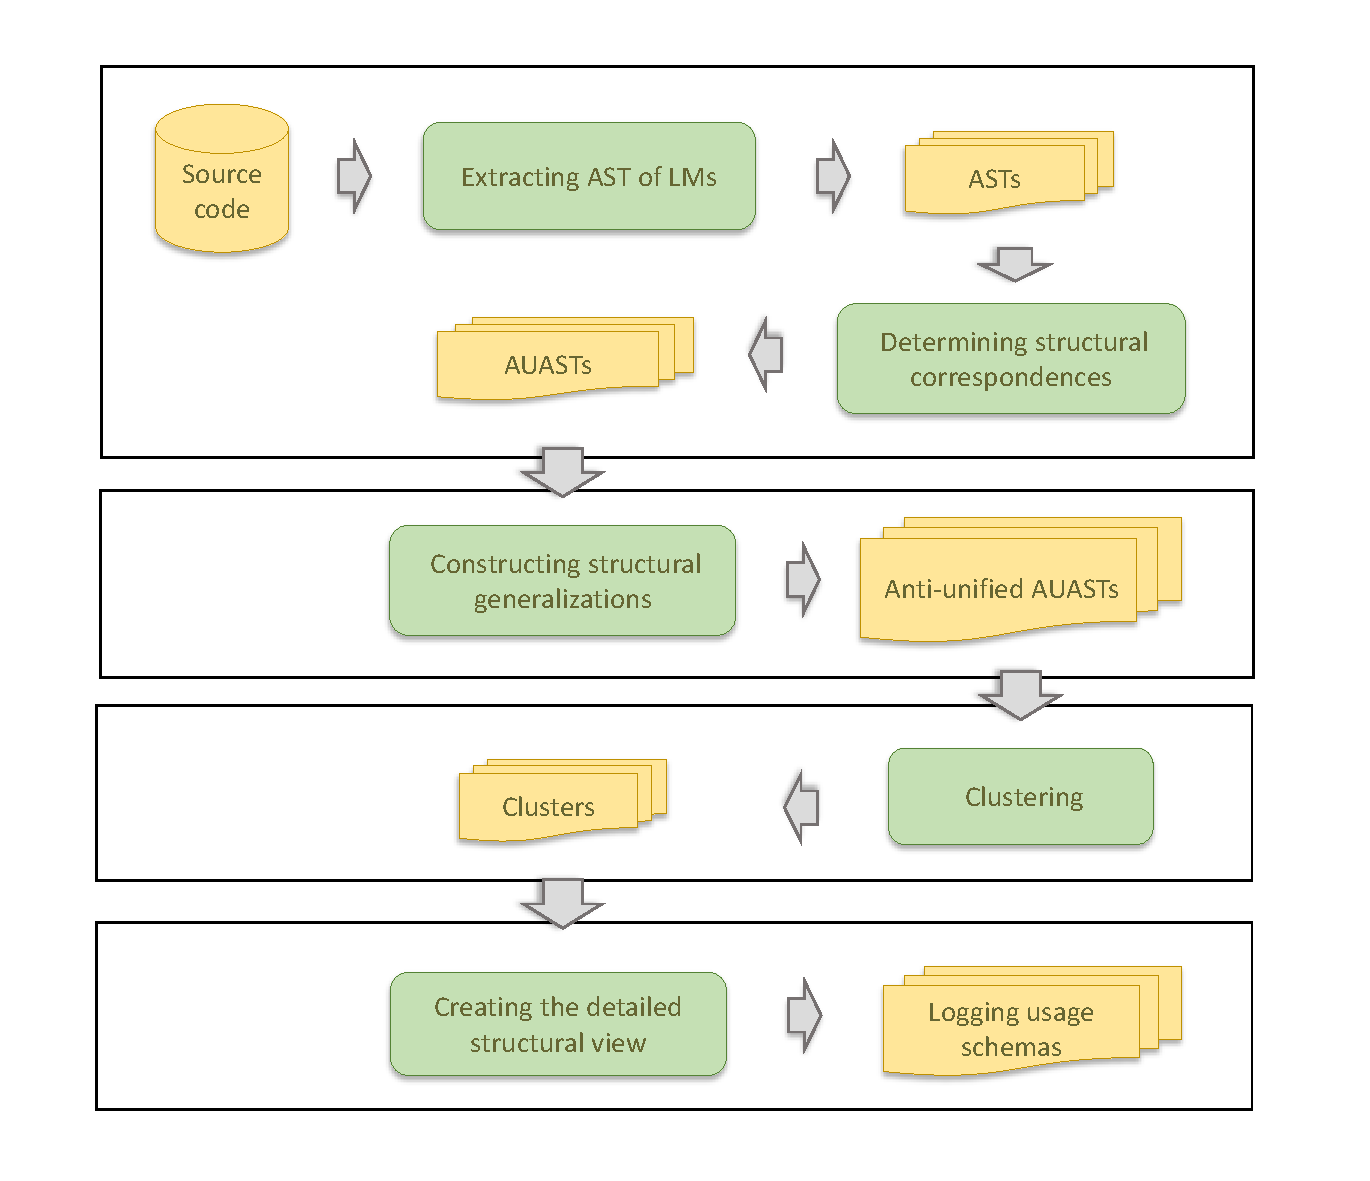
\includegraphics [width = \textwidth]{Drawing4/SystemOverview.pdf}
  \caption{Overview of the approach. \protect\RW{I don't want to see mention of tools here.  This should be focused on the concepts.}} 
  \label{fig:system_overview}
\end{figure}

%most similar  or best correspondence?
%constraints wording?
%my emprical study?
%My tool has been applied on the source code of these systems and extracts all logged Java methods from these systems to construct the structural generalizations.
%My evaluation shows ...

\section{Thesis statement} \label{intro-stmt}
The thesis of this work is that the detailed structural similarities and differences between source code that makes use of logging calls can be determined via higher-order anti-unification modulo theories, providing a concise and accurate description of where logging calls do occur in real-world software systems.
%via HOAUMT and clustering???

\section{Thesis organization} \label{intro-org}
The remainder of the thesis is organized as follows. 

Chapter~\ref{ch2} motivates the problem of understanding where to use logging calls in source code through a scenario in which a developer attempts to perform a logging task. This scenario outlines the potential problems she may encounter and illustrates that the current logging practice is insufficiently supported.

Chapter~\ref{background} provides background information that I build atop: abstract syntax trees (ASTs), which are the basic structure I will use for describing software source code; anti-unification, which is a theoretical approach for determining similarities and differences in tree structures; the Eclipse JDT, an industrial framework for producing and manipulating ASTs for source code written in the Java programming language; and on Jigsaw, a research tool based on the Eclipse JDT for performing anti-unification.

\RW{This chapter needs to be clearer about what is new and what is not. By moving all background to the earlier chapter, this is better but not quite good enough.  You can then have this chapter be explicit about what you added and you can have the reader be less lost in the details.  Currently, you start the chapter with an algorithm that they cannot possibly understand because you have not yet explained the background.  That's bad.  With the structure I specified above, the background will all be in the previous chapter.  Now, the reader will be able to appreciate what you are trying to do.  The following description will need to be modified.}


Chapters~\ref{background2},~\ref{methodology}, and~\ref{clustering} present the first three steps of my approach to determining structural correspondences between AUASTs, constructing structural generalizations from an AUAST pair, and classifying a set of AUASTs into separate clusters, respectively. In each chapter, I discussed the implementation of my approach as an Eclipse plug-in, and conducted an experimental study to assess the effectiveness of my approach through the application of its tool support on a sample test suite extracted from a real software system.


%. Chapters~\ref{background2} described my approach to determining candidate structural correspondences, its supporting tool built atop Jigsaw, and the experimental study on a set of LJMs selected form a real software system to validate the effectiveness of Jigsaw for my application.

%Chapter~\ref{methodology} presents my anti-unification approach as a set of novel algorithms, and its implementation as a plug-in to the Eclipse integrated development environment (IDE),and my experimental study to assess the effectiveness of my approach and the tool support in constructing structural generalizations and computing similarity between structures.
%Chapter~\ref{methodology} describes the clustering algorithm, its tool support, and an . \RW{This paragraph needs modification.}


%The first study is conducted to evaluate the accuracy of my approach and its implemented tool by conducting an experiment on 10 sample logged Java methods.
Chapter~\ref{eval} presents an empirical study I conducted to characterize the location of logging usage in three open-source software systems. Chapter~\ref{diss} discusses the results and findings of my work, threats to its validity, and the remaining issues. Chapter~\ref{rw} describes work related to my research problem and how it does not adequately address the problem. Chapter~\ref{conc} concludes the dissertation and presents the contributions of this study and future work. %Additional materials appended this dissertation are provided in Appendix A.


% difference between experimental or emiprical study



\addtocontents{toc}{\protect\addvspace{10pt}}
\chapter{Motivational Scenario}  \label{ch2}

Printing messages to the console or to a log file is an integral part of software development and can be used to test, debug, and understand what is happening inside an application. In the Java programming language, \name{print} statements are commonly used to print something on console. However, the availability of tools, frameworks, and APIs for logging that offers more powerful and advanced Java logging features, flexibility, and improvement in the logging quality suggests that using \name{print} statements is not sufficient to perform logging practices in real-world applications.
%?
% Java Logging API

The logging frameworks offer many more facilities that are not provided by the \name{print} statements. For example, most logging frameworks (e.g., \name{log4j}, \name{SLF4J}, \name{java.util.logging}) use different verbosity levels to control the types of information needed to be logged. That is, by logging at a particular verbosity level, logs at that level and higher levels will be recorded whereas the logs at lower levels will be discarded. Each of these verbosity levels can be used for different applications during software development. For example, the \name{debug} log level messages can be used in a test environment, while the \name{error} log level messages can be used in a production environment. This feature not only produces fewer log messages for each level, but also improves the performance of an application. Also, most logging frameworks allow the production of formatted log messages, which makes it easier for a developer to monitor the behavior of a system. In addition, when a developer is working on a server side application, the only way to know what is happening inside the server is by monitoring the log files. Although logging is a valuable practice for software development and maintenance, it imposes extra time and energy on developers to write, test, and run the code, while affecting the application performance. As latency and speed are major concerns for most software systems, it is necessary for a developer to understand and learn logging practices in great detail in order to perform them in an efficient manner.

To illustrate the inherent challenges of effectively performing logging practices in software systems, one may consider a scenario in which a developer is asked to log an event-based mechanism of a text editor tool written in the Java programming language. In this scenario, the developer is trying to log a Java class of the system (Figure~\ref{ch2-ex}) using the \name{Apache log4j} framework. She knows that components of this application register with the \name{EditBus} class to receive messages that reflect changes in the application's state, and that the \name{EditBus} class maintains a list of components that have requested to receive messages. That is, when a message is sent using this class, all registered components receive it in turn. Furthermore, any classes that subscribe to the \name{EditBus} and implement the \code{EBComponent} interface define the method \code{EBComponent.handleMessage(EBMessage)} to handle a message sent on by the \code{EditBus}. To perform this logging task, the developer might ask herself several fundamental questions, mostly related to where and what to log.
% Example is a class, not a method. Is it ok???


\begin{figure}[p]
\def\baselinestretch{1}
\begin{lstlisting}
public class EditBus {
    private static ArrayList components = new ArrayList();
    private static EBComponent[] copyComponents;

    private EditBus() {
    }

    public static void addToBus(EBComponent comp) {
        synchronized(components) {
            components.add(comp);
            copyComponents = null;
        }
    }

    public static void removeFromBus(EBComponent comp) {
        synchronized(components) {
            components.remove(comp);
            copyComponents = null;
        }
    }

    public static EBComponent[] getComponents() {
        synchronized(components) {
            if(copyComponents == null) {
                EBComponent[] arr = new EBComponent[components.size()];
                copyComponents =
                    (EBComponent[])components.toArray(arr);
            }
        }
        return copyComponents;
    }

    public static void send(EBMessage message) {
        EBComponent[] comps = getComponents();
        for(int i = 0; i < comps.length; i++) {
            EBComponent comp = comps[i];
            long start = System.currentTimeMillis();
            comp.handleMessage(message);
            long time = (System.currentTimeMillis() - start);
        }
    }
}
\end{lstlisting}
\caption{The \code{EditBus} class.\label{ch2-ex}}
\end{figure}
%Developer's logging task context on

Her first solution might be to simply log at the start and end of every method. However, she believes that logging at the start and end of the \code{addToBus(EBComponent)}, \code{remove}\-\code{From}\-\code{Bus(EBComponent)}, and \code{getComponents()} methods are useless, and will produce redundant information. She assumes that the more she logs, the more she performs file I/O, which slows down the application. Therefore, she decides to log only important information necessary to debug or troubleshoot potential problems. She proceeds to identify the information needed to be logged and then decides on where to use log statements. She thinks that it is important to log the information related to a message sent to a registered component, including the message content and the transmission time, to find the root causes of potential problems in sending messages. She simply wants to begin by using a log statement at the start of the \code{send()} method (line~2 of Figure~\ref{ch2-ex-logged-m1}) to log the information. However, she realizes that this log statement does not allow her to log all the information she wants, as the \code{time} variable is not initialized at the beginning of this method. Therefore, she proceeds to examine the body of the \code{send()} method line-by-line and uses another log statement after the \code{time} variable is initialized. She aims to log the transmission time in case of potential problems in sending messages. Therefore, she decides to insert the logging call inside an \code{if} statement that logs the value of the variable \code{time}, if it is not within a valid range (shown in lines~9--11 of Figure~\ref{ch2-ex-logged-m2}).
%She aims to log the transmission time in case of potential problems in sending messages.?

\begin{figure}[p]
\def\baselinestretch{1}
\begin{lstlisting}[escapechar=!]
public static void send(EBMessage message){
   !\colorbox{yellowGreen}{//log statement}!
   EBComponent[] comps = getComponents();
   for (int i = 0; i < comps.length; i++) {
       EBComponent comp = comps[i];
       long start = System.currentTimeMillis();
       comp.handleMessage(message);
       long time = (System.currentTimeMillis() - start);
   }
}
\end{lstlisting}
\caption[The developer's initial determination of the usage of logging calls.]{The developer's initial determination of the usage of log statements for the \code{send(EBMessage)} method.\label{ch2-ex-logged-m1}}
\end{figure}

\begin{figure}[p]
\def\baselinestretch{1}
\begin{lstlisting}[escapechar=!]
public static void send(EBMessage message) {
    !\colorbox{yellowGreen}{//log statement}!
    EBComponent[] comps = getComponents();
    for(int i = 0; i < comps.length; i++) {
        EBComponent comp = comps[i];
        long start = System.currentTimeMillis();
        comp.handleMessage(message);
        long time = (System.currentTimeMillis() - start);
        if(time >= 1000000) {
            !\colorbox{yellowGreen}{//log statement}!
        }
    }
}
\end{lstlisting}
\caption[The developer's second determination of the usage of log statements.]{The developer's second determination of the usage of log statements for the \code{send(EBMessage)} method.\label{ch2-ex-logged-m2}}
\end{figure}

\begin{figure}[p]
\def\baselinestretch{1}
\begin{lstlisting}[escapechar=!]
public static void send(EBMessage message){
    try {
        !\colorbox{yellowGreen}{//log statement}!
        EBComponent[] comps = getComponents();
        for(int i = 0; i < comps.length; i++) {
            EBComponent comp = comps[i];
            long start = System.currentTimeMillis();
            comp.handleMessage(message);
            long time = (System.currentTimeMillis() - start);
            if(time >= 1000000) {
                !\colorbox{yellowGreen}{//log statement}!
            }
        }
    } catch(Throwable t) {
       !\colorbox{yellowGreen}{//log statement}!
    }
}
\end{lstlisting}
\caption[The developer's third determination of the usage of log statements.]{The developer's third determination of the usage of log statements for the \code{send(EBMessage)} method.\label{ch2-ex-logged-m3}}
\end{figure}

She also believes that it is important to log an error if any problems occur in sending messages to the components. She decides to use a \code{try}/\code{catch} statement, as it is a common way to handle exceptions in the Java programming language. She creates a \code{try}/\code{catch} block to capture the potential failure in sending messages, and uses a log statement inside the \code{catch} block to log the exception (shown in lines~2--16 of Figure~\ref{ch2-ex-logged-m3}). However, she realizes that using this logging call will not allow her to reach the desired functionality, as it does not reveal to which component the problem is related. Thus, she decides to relocate the \code{try}/\code{catch} block inside the \code{for} statement to log an error in case of a problem in sending messages to any components (shown in lines~5--15 of Figure~\ref{ch2-ex-logged-m4}).


\begin{figure}[p]
\def\baselinestretch{1}
\begin{lstlisting}[escapechar=!]
public static void send(EBMessage message) {
    !\colorbox{yellowGreen}{//log statement}!
    EBComponent[] comps = getComponents();
    for (int i = 0; i < comps.length; i++) {
        try {
            EBComponent comp = comps[i];
            long start = System.currentTimeMillis();
            comp.handleMessage(message);
            long time = (System.currentTimeMillis() - start);
            if(time >= 1000000) {
                !\colorbox{yellowGreen}{//log statement}!
            }
        } catch(Throwable t) {
            !\colorbox{yellowGreen}{//log statement}!
        }
    }
}
\end{lstlisting}
\caption[The developer's fourth determination of the usage of log statements.]{The developer's fourth determination of the usage of log statements for the \code{send(EBMessage)} method.\label{ch2-ex-logged-m4}}
\end{figure}

\begin{figure}[p]
\def\baselinestretch{0.94}
\begin{lstlisting}[escapechar=!]
public class EditBus {
    private static ArrayList components = new ArrayList();
    private static EBComponent[] copyComponents;

    private EditBus() {
    }

    public static void addToBus(EBComponent comp) {
        synchronized(components) {
            components.add(comp);
            copyComponents = null;
        }
    }

    public static void removeFromBus(EBComponent comp) {
        synchronized(components) {
            components.remove(comp);
            copyComponents = null;
        }
    }

    public static EBComponent[] getComponents() {
        synchronized(components) {
            if(copyComponents == null) {
                EBComponent[] arr = new EBComponent[components.size()];
                copyComponents = (EBComponent[])components.toArray(arr);
            }
        }
        return copyComponents;
    }

    public static void send(EBMessage message) {
        !\colorbox{yellowGreen}{//log statement}!
        EBComponent[] comps = getComponents();
        for(int i = 0; i < comps.length; i++) {
            try {
                EBComponent comp = comps[i];
                long start = System.currentTimeMillis();
                comp.handleMessage(message);
                long time = (System.currentTimeMillis() - start);
                if(time >= 1000000) {
                    !\colorbox{yellowGreen}{//log statement}!
                }
            } catch(Throwable t) {
                 !\colorbox{yellowGreen}{//log statement}!
            }
        }
    }
}
\end{lstlisting}

\caption[The developer's final determination of the usage of log statements.]{The developer's final determination of the usage of log statements for the \code{EditBus} class.\label{ch2-ex-logged}}
\end{figure}

%which information or what?
Figure~\ref{ch2-ex-logged} shows the developer's final determination of the usage of log statements to perform the logging task of the \code{EditBus} class. By making appropriate decisions about where to use log statements, the developer is in a good position to proceed to write the logging messages by examining the remaining conceptually complex questions. What specific information should I log? How should I choose the log message format? Which information goes to which level of logging? If the developer had reached this point more easily and quickly, she would have had more time and energy to make decisions about the remaining issues and could have completed the logging practice in a timely and appropriate manner.

%\RW{This is followed by a summary, so it is rather redundant.}
%To sum up, this scenario required the developer to make numerous decisions and then act on them. Her attention was split between detailed and the high-level decisions. In addition, time constraints and the performance of tedious tasks can cause the developer to make bad decisions. However, having a vision of where developers usually use logging calls in similar situations could guide her to make informed decisions about where to use logging calls, and she could then perform the logging task in a faster and less error-prone manner.


\section{Summary}  \label{ch2-summary}

This motivational scenario highlights the problems a developer may encounter in performing a logging task. The core problem she faces in this scenario is the difficulty in understanding where to use log statements that enable her to log the desired information. However, having an understanding of how developers usually log in similar situations might assist her to make informed decisions about where to use log statements more effectively, and so she could pay more attention to the remaining, conceptually complex issues to complete the logging task.

% where to use log statements more effectively
%comma???
%in a faster and less error-prone manner



\addtocontents{toc}{\protect\addvspace{10pt}}
%\chapter{Background}  \label{background}
\chapter{Background}  \label{background}
A programming language is described by the combination of its syntax and semantics. The syntax concerns the legal structures of programs written in the programming language, while the semantics is about the meaning of every construct in that language. Furthermore, the abstract syntactic structure of source code written in a programming language can be represented as an \emph{abstract syntax tree} (AST), in which nodes are occurrences of syntactic structures and edges represent nesting relationships. Since ASTs will be the form in which I represent and analyze source code, I need a means to generalize sets of ASTs in order to understand their commonalities while abstracting away their differences. The theoretical framework of anti-unification is presented as that means.

In this chapter, ASTs are described in Section~\ref{AST}, along with their more concrete counterparts, concrete syntax trees. A specific, industrial framework for creating and manipulating ASTs for source code written in the Java programming language---the Eclipse JDT---is described in Section~\ref{JDT}.  Anti-unification is summarized in Section~\ref{AU}, starting with its most basic form, first-order anti-unification, and progressing to the form that I will make use of, higher-order anti-unification modulo equational theories, in Section~\ref{HOAUMT}.  A research approach, built atop the Eclipse JDT, for performing anti-unification on Java ASTs---the Jigsaw framework---is described in Section~\ref{Jigsaw}. In the last section of this chapter, I provide some background information about clustering, existing clustering techniques, and the agglomerative hierarchical clustering algorithm, as a technique I used to cluster logged methods into separate groups based on a similarity measurement.
%AHC???
% as a technique or the technique??

\section{Concrete syntax trees and abstract syntax trees}\label{AST}

A concrete syntax tree is a tree $T=(V,E)$ whose vertices $V$ (equivalently, nodes) represent the syntactic structures (equivalently, syntactic elements) of a specific program written in a specific programming language and whose directed edges $E$ represent the nesting relationships amongst those syntactic structures.  Non-leaf nodes in a concrete syntax tree (also called a parse tree) represent the grammar productions that were satisfied in parsing the program it represents; leaf nodes represent the concrete lexemes, such as literals and keywords.

I focus on the Java programming language and I make use of the grammar in the language specification \cite[][Chapter 18]{2012:book:gosling} to determine the form of the concrete syntax trees.  Non-leaf node names are represented by names in ``camel-case'' written in italics.  Consider the trivial program in Figure~\ref{fig:java-example}; its concrete syntax tree is represented in Figure~\ref{fig:java-example-cst}.

\begin{figure}
\begin{lstlisting}
public class HelloWorld {
    public static void main(String[] args) {
        System.out.println("Hello world!");
    }
}
\end{lstlisting}
\caption{A simple example Java program.\label{fig:java-example}}
\end{figure}

\begin{sidewaysfigure}
\centering\resizebox{!}{0.65\textheight}{%
\begin{tikzpicture}
\node(cu) at (-14,20) {\textit{compilationUnit}};
%
\node(td) at (-14,19) {\textit{typeDeclaration}};
\draw[->](cu) -- (td) {};
%
\node(cid) at (-14,18) {\textit{classOrInterfaceDeclaration}};
\draw[->](td) -- (cid) {};
%
\node(mod2) at (-16,17) {\textit{modifier}};
\draw[->](cid) -- (mod2) {};
%
\node(public2) at (-16,16) {\textsf{\small public}};
\draw[->](mod2) -- (public2) {};
%
\node(cd) at (-12,17) {\textit{classDeclaration}};
\draw[->](cid) -- (cd) {};
%
\node(ncd) at (-12,16) {\textit{normalClassDeclaration}};
\draw[->](cd) -- (ncd) {};
%
\node(class) at (-16,15) {\textsf{\small class}};
\node(id7) at (-14,15) {\textit{identifier}};
\node(cbody) at (-8,15) {\textit{classBody}};
\draw[->](ncd) -- (class) {};
\draw[->](ncd) -- (id7) {};
\draw[->](ncd) -- (cbody) {};
%
\node(HelloWorld) at (-14,14) {\textsf{\small HelloWorld}};
\draw[->](id7) -- (HelloWorld) {};
%
\node(obr2) at (-12,14) {\textsf{\small \{}};
\node(cbd) at (-8,14) {\textit{classBodyDeclaration}};
\node(cbr2) at (-4,14) {\textsf{\small \}}};
\draw[->](cbody) -- (obr2) {};
\draw[->](cbody) -- (cbd) {};
\draw[->](cbody) -- (cbr2) {};
%
\node(mod1) at (-12,13) {\textit{modifier}};
\node(mod2) at (-10,13) {\textit{modifier}};
\node(md) at (-4,13) {\textit{memberDecl}};
\draw[->](cbd) -- (mod1) {};
\draw[->](cbd) -- (mod2) {};
\draw[->](cbd) -- (md) {};
%
\node(public1) at (-12,12) {\textsf{\small public}};
\draw[->](mod1) -- (public1) {};
%
\node(static) at (-10,12) {\textsf{\small static}};
\draw[->](mod2) -- (static) {};
%
\node(void) at (-8,12) {\textsf{\small void}};
\node(id6) at (-6,12) {\textit{identifier}};
\node(vmdr) at (2,12) {\textit{voidMethodDeclaratorRest}};
\draw[->](md) -- (void) {};
\draw[->](md) -- (id6) {};
\draw[->](md) -- (vmdr) {};
%
\node(main) at (-6,11) {\textsf{\small main}};
\draw[->](id6) -- (main) {};
%
\node(formals) at (-2,11) {\textit{formalParameters}};
\draw[->](vmdr) -- (formals) {};
%
\node(op2) at (-5,10) {\textsf{\small (}};
\node(fpd) at (-2,10) {\textit{formalParameterDecls}};
\node(cp2) at (1,10) {\textsf{\small )}};
\draw[->](formals) -- (op2) {};
\draw[->](formals) -- (fpd) {};
\draw[->](formals) -- (cp2) {};
%
\node(type) at (-4,9) {\textit{type}};
\node(fpdr) at (0,9) {\textit{formalParameterDeclsRest}};
\draw[->](fpd) -- (type) {};
\draw[->](fpd) -- (fpdr) {};
%
\node(rt) at (-6,8) {\textit{referenceType}};
\node(obt) at (-4,8) {\textsf{\small [}};
\node(cbt) at (-3,8) {\textsf{\small ]}};
\draw[->](type) -- (rt) {};
\draw[->](type) -- (obt) {};
\draw[->](type) -- (cbt) {};
%
\node(id5) at (-6,7) {\textit{identifier}};
\draw[->](rt) -- (id5) {};
%
\node(String) at (-6,6) {\textsf{\small String}};
\draw[->](rt) -- (String) {};
%
\node(vdi) at (0,8) {\textit{variableDeclaratorId}};
\draw[->](fpdr) -- (vdi) {};
%
\node(id4) at (0,7) {\textit{identifier}};
\draw[->](vdi) -- (id4) {};
%
\node(args) at (0,6) {\textsf{\small args}};
\draw[->](id4) -- (args) {};
%
\node(block) at (6,11) {\textit{block}};
\draw[->](vmdr) -- (block) {};
%
\node(obrace1) at (4,10) {\textsf{\small \{}};
\node(bs1) at (6,10) {\textit{blockStatements}};
\node(cbrace1) at (8,10) {\textsf{\small \}}};
\draw[->](block) -- (obrace1) {};
\draw[->](block) -- (bs1) {};
\draw[->](block) -- (cbrace1) {};
%
\node(bs2) at (6,9) {\textit{blockStatement}};
\draw[->](bs1) -- (bs2) {};
%
\node(stat) at (6,8) {\textit{statement}};
\draw[->](bs2) -- (stat) {};
%
\node(se) at (5,7) {\textit{statementExpression}};
\node(sc) at (7.5,7) {\textsf{\small ;}};
\draw[->](stat) -- (se) {};
\draw[->](stat) -- (sc) {};
%
\node(expr) at (5,6) {\textit{expression}};
\draw[->](se) -- (expr) {};
%
\node(e1) at (5,5) {\textit{expression1}};
\draw[->](expr) -- (e1) {};
%
\node(e2) at (5,4) {\textit{expression2}};
\draw[->](e1) -- (e2) {};
%
\node(e3) at (5,3) {\textit{expression3}};
\draw[->](e2) -- (e3) {};
%
\node(prim1) at (2,2) {\textit{primary}};
\node(sel) at (8,2) {\textit{selector}};
\draw[->](e3) -- (prim1) {};
\draw[->](e3) -- (sel) {};
%
\node(id1) at (0,1) {\textit{identifier}};
\node(dot1) at (2,1) {\textsf{\small .}};
\node(id2) at (4,1) {\textit{identifier}};
\draw[->](prim1) -- (id1) {};
\draw[->](prim1) -- (dot1) {};
\draw[->](prim1) -- (id2) {};
%
\node(dot2) at (6,1) {\textsf{\small .}};
\node(id3) at (8,1) {\textit{identifier}};
\node(arguments) at (11,1) {\textit{arguments}};
\draw[->](sel) -- (dot2) {};
\draw[->](sel) -- (id3) {};
\draw[->](sel) -- (arguments) {};
%
\node(System) at (0,0) {\textsf{\small System}};
\draw[->](id1) -- (System) {};
%
\node(out) at (4,0) {\textsf{\small out}};
\draw[->](id2) -- (out) {};
%
\node(println) at (8,0) {\textsf{\small println}};
\draw[->](id3) -- (println) {};
%
\node(op) at (9,0) {\textsf{\small (}};
\node(sl) at (11,0) {\textsf{\small "Hello world!"}};
\node(cp) at (13,0) {\textsf{\small )}};
\draw[->](arguments) -- (op) {};
\draw[->](arguments) -- (sl) {};
\draw[->](arguments) -- (cp) {};
\end{tikzpicture}%
}
\caption{The concrete syntax tree for the program of Figure~\ref{fig:java-example}.\label{fig:java-example-cst}}
\end{sidewaysfigure}

Beyond the fact that the concrete syntax tree is rather verbose and thus occupies a lot of space even for a trivial example, I can see two key problems with it: (1)~there are a multitude of redundant nodes such as \textit{expression1}, \textit{expression2}, and \textit{expression3} that are present solely for purposes of creating an unambiguous grammar; and (2)~there are no nodes that express key concepts, such as ``method declaration'' and ``method invocation'', that should be obviously present in the example program.

To address these problems, concrete syntax trees are converted to abstract syntax trees (ASTs). An AST is similar in concept to a concrete syntax tree but it does not generally represent the parsing steps followed to differentiate different kinds of syntactic structure. The node types are chosen to represent syntactical concepts; I use the grammar presented for exposition by \citet{2012:book:gosling}, which differs markedly from the grammar they propose in their Chapter~18 for efficient parsing. Note that a given node type constrains the kinds and numbers of child nodes that it possesses. The AST derived from the concrete syntax tree of Figure~\ref{fig:java-example-cst} is shown in Figure~\ref{fig:java-example-ast}. Note that, although I know that (for any normal program) \code{System} refers to the class \code{java.lang.System} and \code{out} is a static field on that class, non-normal programs can occur and a pure syntactic analysis cannot rule out that \code{System} is a package and that \code{out} is a class therein declaring a static method \code{println(String)}.

\begin{sidewaysfigure}
\centering\resizebox{!}{0.4\textheight}{%
\begin{tikzpicture}
\node(cu) at (-12,11) {\textit{compilationUnit}};
%
\node(cd) at (-12,10) {\textit{classDeclaration}};
\draw[->](cu) -- (cd) {};
%
\node(mod3) at (-16,9) {\textit{modifier}};
\node(class) at (-14,9) {\textsf{\small class}};
\node(id7) at (-12,9) {\textit{identifier}};
\node(cbody) at (-4,9) {\textit{classBody}};
\draw[->](cd) -- (mod3) {};
\draw[->](cd) -- (class) {};
\draw[->](cd) -- (id7) {};
\draw[->](cd) -- (cbody) {};
%
\node(public2) at (-16,8) {\textsf{\small public}};
\draw[->](mod3) -- (public2) {};
%
\node(HelloWorld) at (-12,8) {\textsf{\small HelloWorld}};
\draw[->](id7) -- (HelloWorld) {};
%
\node(obr2) at (-8,8) {\textsf{\small \{}};
\node(md) at (-4,8) {\textit{methodDeclaration}};
\node(cbr2) at (0,8) {\textsf{\small \}}};
\draw[->](cbody) -- (obr2) {};
\draw[->](cbody) -- (md) {};
\draw[->](cbody) -- (cbr2) {};
%
\node(mod1) at (-12,6) {\textit{modifier}};
\node(mod2) at (-10,6) {\textit{modifier}};
\node(result) at (-8,6) {\textit{result}};
\node(id6) at (-6,6) {\textit{identifier}};
\node(fps) at (-2,6) {\textit{formalParameters}};
\node(mbody) at (6,6) {\textit{methodBody}};
\draw[->](md) -- (mod1) {};
\draw[->](md) -- (mod2) {};
\draw[->](md) -- (result) {};
\draw[->](md) -- (id6) {};
\draw[->](md) -- (fps) {};
\draw[->](md) -- (mbody) {};
%
\node(public1) at (-12,5) {\textsf{\small public}};
\draw[->](mod1) -- (public1) {};
%
\node(static) at (-10,5) {\textsf{\small static}};
\draw[->](mod2) -- (static) {};
%
\node(void) at (-8,5) {\textsf{\small void}};
\draw[->](result) -- (void) {};
%
\node(main) at (-6,5) {\textsf{\small main}};
\draw[->](id6) -- (main) {};
%
\node(op2) at (-4,5) {\textsf{\small (}};
\node(fp) at (-2,5) {\textit{formalParameter}};
\node(cp2) at (0,5) {\textsf{\small )}};
\draw[->](fps) -- (op2) {};
\draw[->](fps) -- (fp) {};
\draw[->](fps) -- (cp2) {};
%
\node(type) at (-4,4) {\textit{arrayType}};
\node(id5) at (0,4) {\textit{identifier}};
\draw[->](fp) -- (type) {};
\draw[->](fp) -- (id5) {};
%
\node(id4) at (-6,3) {\textit{identifier}};
\node(obt) at (-4,3) {\textsf{\small [}};
\node(cbt) at (-2,3) {\textsf{\small ]}};
\node(args) at (0,3) {\textsf{\small args}};
\draw[->](type) -- (id4) {};
\draw[->](type) -- (obt) {};
\draw[->](type) -- (cbt) {};
\draw[->](id5) -- (args) {};
%
\node(String) at (-6,2) {\textsf{\small String}};
\draw[->](id4) -- (String) {};
%
\node(obrace1) at (4,5) {\textsf{\small \{}};
\node(stat) at (6,5) {\textit{statement}};
\node(cbrace1) at (8,5) {\textsf{\small \}}};
\draw[->](mbody) -- (obrace1) {};
\draw[->](mbody) -- (stat) {};
\draw[->](mbody) -- (cbrace1) {};
%
\node(mi) at (6,4) {\textit{methodInvocation}};
\node(sc) at (8,4) {\textsf{\small ;}};
\draw[->](stat) -- (mi) {};
\draw[->](stat) -- (sc) {};
%
%
\node(qual) at (3,3) {\textit{qualifier}};
\node(id3) at (6,3) {\textit{identifier}};
\node(arguments) at (10,3) {\textit{arguments}};
\draw[->](mi) -- (qual) {};
\draw[->](mi) -- (id3) {};
\draw[->](mi) -- (arguments) {};
%
\node(qn) at (2,2) {\textit{qualifiedName}};
\node(dot2) at (4,2) {\textsf{\small .}};
\node(println) at (6,2) {\textsf{\small println}};
\node(op) at (8,2) {\textsf{\small (}};
\node(sl) at (10,2) {\textsf{\small "Hello world!"}};
\node(cp) at (12,2) {\textsf{\small )}};
\draw[->](qual) -- (qn) {};
\draw[->](qual) -- (dot2) {};
\draw[->](id3) -- (println) {};
\draw[->](arguments) -- (op) {};
\draw[->](arguments) -- (sl) {};
\draw[->](arguments) -- (cp) {};
%
\node(id1) at (0,1) {\textit{identifier}};
\node(dot1) at (2,1) {\textsf{\small .}};
\node(id2) at (4,1) {\textit{identifier}};
\draw[->](qn) -- (id1) {};
\draw[->](qn) -- (dot1) {};
\draw[->](qn) -- (id2) {};
%
\node(System) at (0,0) {\textsf{\small System}};
\draw[->](id1) -- (System) {};
%
\node(out) at (4,0) {\textsf{\small out}};
\draw[->](id2) -- (out) {};
\end{tikzpicture}%
}
\caption{The abstract syntax tree derived from the concrete syntax tree of Figure~\ref{fig:java-example-cst}.\label{fig:java-example-ast}}
\end{sidewaysfigure}

This is still verbose, so in practice we elide details that are implied or otherwise trivial, to arrive at a more abstract AST as shown in Figure~\ref{fig:java-example-ast2}.

\begin{sidewaysfigure}
\centering\resizebox{!}{0.4\textheight}{%
\begin{tikzpicture}
\node(cu) at (-12,11) {\textit{compilationUnit}};
%
\node(cd) at (-12,10) {\textit{classDeclaration}};
\draw[->](cu) -- (cd) {};
%
\node(HelloWorld) at (-12,8) {\textsf{\small HelloWorld}};
\draw[->](cd) -- (HelloWorld) {};
%
\node(md) at (-4,8) {\textit{methodDeclaration}};
\draw[->](cd) -- (md) {};
%
\node(result) at (-8,6) {\textit{result}};
\node(fps) at (-2,6) {\textit{formalParameters}};
\node(mbody) at (6,6) {\textit{methodBody}};
\draw[->](md) -- (result) {};
\draw[->](md) -- (fps) {};
\draw[->](md) -- (mbody) {};
%
\node(void) at (-8,5) {\textsf{\small void}};
\draw[->](result) -- (void) {};
%
\node(main) at (-6,5) {\textsf{\small main}};
\draw[->](md) -- (main) {};
%
\node(fp) at (-2,5) {\textit{formalParameter}};
\draw[->](fps) -- (fp) {};
%
\node(type) at (-4,4) {\textit{arrayType}};
\draw[->](fp) -- (type) {};
%
\node(args) at (0,3) {\textsf{\small args}};
\draw[->](fp) -- (args) {};
%
\node(String) at (-6,2) {\textsf{\small String}};
\draw[->](type) -- (String) {};
%
\node(mi) at (6,4) {\textit{methodInvocation}};
\draw[->](mbody) -- (mi) {};
%
\node(arguments) at (10,3) {\textit{arguments}};
\draw[->](mi) -- (arguments) {};
%
\node(qn) at (2,2) {\textit{qualifiedName}};
\node(dot2) at (4,2) {\textsf{\small .}};
\node(println) at (6,2) {\textsf{\small println}};
\node(sl) at (10,2) {\textsf{\small "Hello world!"}};
\draw[->](mi) -- (qn) {};
\draw[->](mi) -- (println) {};
\draw[->](arguments) -- (sl) {};
%
\node(System) at (0,0) {\textsf{\small System}};
\draw[->](qn) -- (System) {};
%
\node(out) at (4,0) {\textsf{\small out}};
\draw[->](qn) -- (out) {};
\end{tikzpicture}%
}
\caption{A more abstract AST derived from the concrete syntax tree of Figure~\ref{fig:java-example-cst}.\label{fig:java-example-ast2}}
\end{sidewaysfigure}

\section{Eclipse JDT}\label{JDT}
The Eclipse Java Development Tools (JDT) framework provides APIs to access and manipulate Java source code via ASTs. An AST represents Java source code in a tree form, where the typed nodes represent instances of certain syntactic structures from the Java programming language. Each node type (in general) takes a set of child nodes, also typed and with certain constraints on their properties.  Groups of children are named on the basis of the conceptual purpose of those groups; optional groups can be empty, which we can represent with the \NIL{} element. %Thus, any Java source code can be represented as a tree of AST nodes.
For example, the simple AST structure of two sample LMs in Figures~\ref{ch3-ex1} an~\ref{ch3-ex2} is shown in Figure~\ref{fig:ast}, with the log statements highlighted in yellow.


\begin{figure}[p]
\def\baselinestretch{1}
\begin{lstlisting}[escapechar=!]
public void handleMessage(EBMessage message) {
   if(seenWarning)
      return;
   seenWarning = true;
   !\colorbox{yellowGreen}{Log.log(Log.WARNING, this, getClassName() + " should extend EditPlugin not EBPlugin}!  !\colorbox{yellowGreen}{since it has an empty " + handleMessage());}!
}
\end{lstlisting}
\caption[Example 1: A Java method that uses a log statement.]{A Java method that uses a log statement. This will be referred to as Example 1.\label{ch3-ex1}}
\end{figure}

\begin{figure}[p]
\def\baselinestretch{1}
\begin{lstlisting}[escapechar=!]
public void actionPerformed(ActionEvent evt) {
   EditAction action = context.getAction(actionName);
   if(action == null) {
      !\colorbox{yellowGreen}{Log.log(Log.ERROR, this, "Unknown action: " + actionName);}!
   }
   else{
      context.invokeAction(evt, action);
   }
}
\end{lstlisting}
\caption[Example 2: A Java method that uses a log statement.]{A Java method that uses a log statement. This will be referred to as Example 2.\label{ch3-ex2}}
\end{figure}

\begin{figure} [p]
  \centering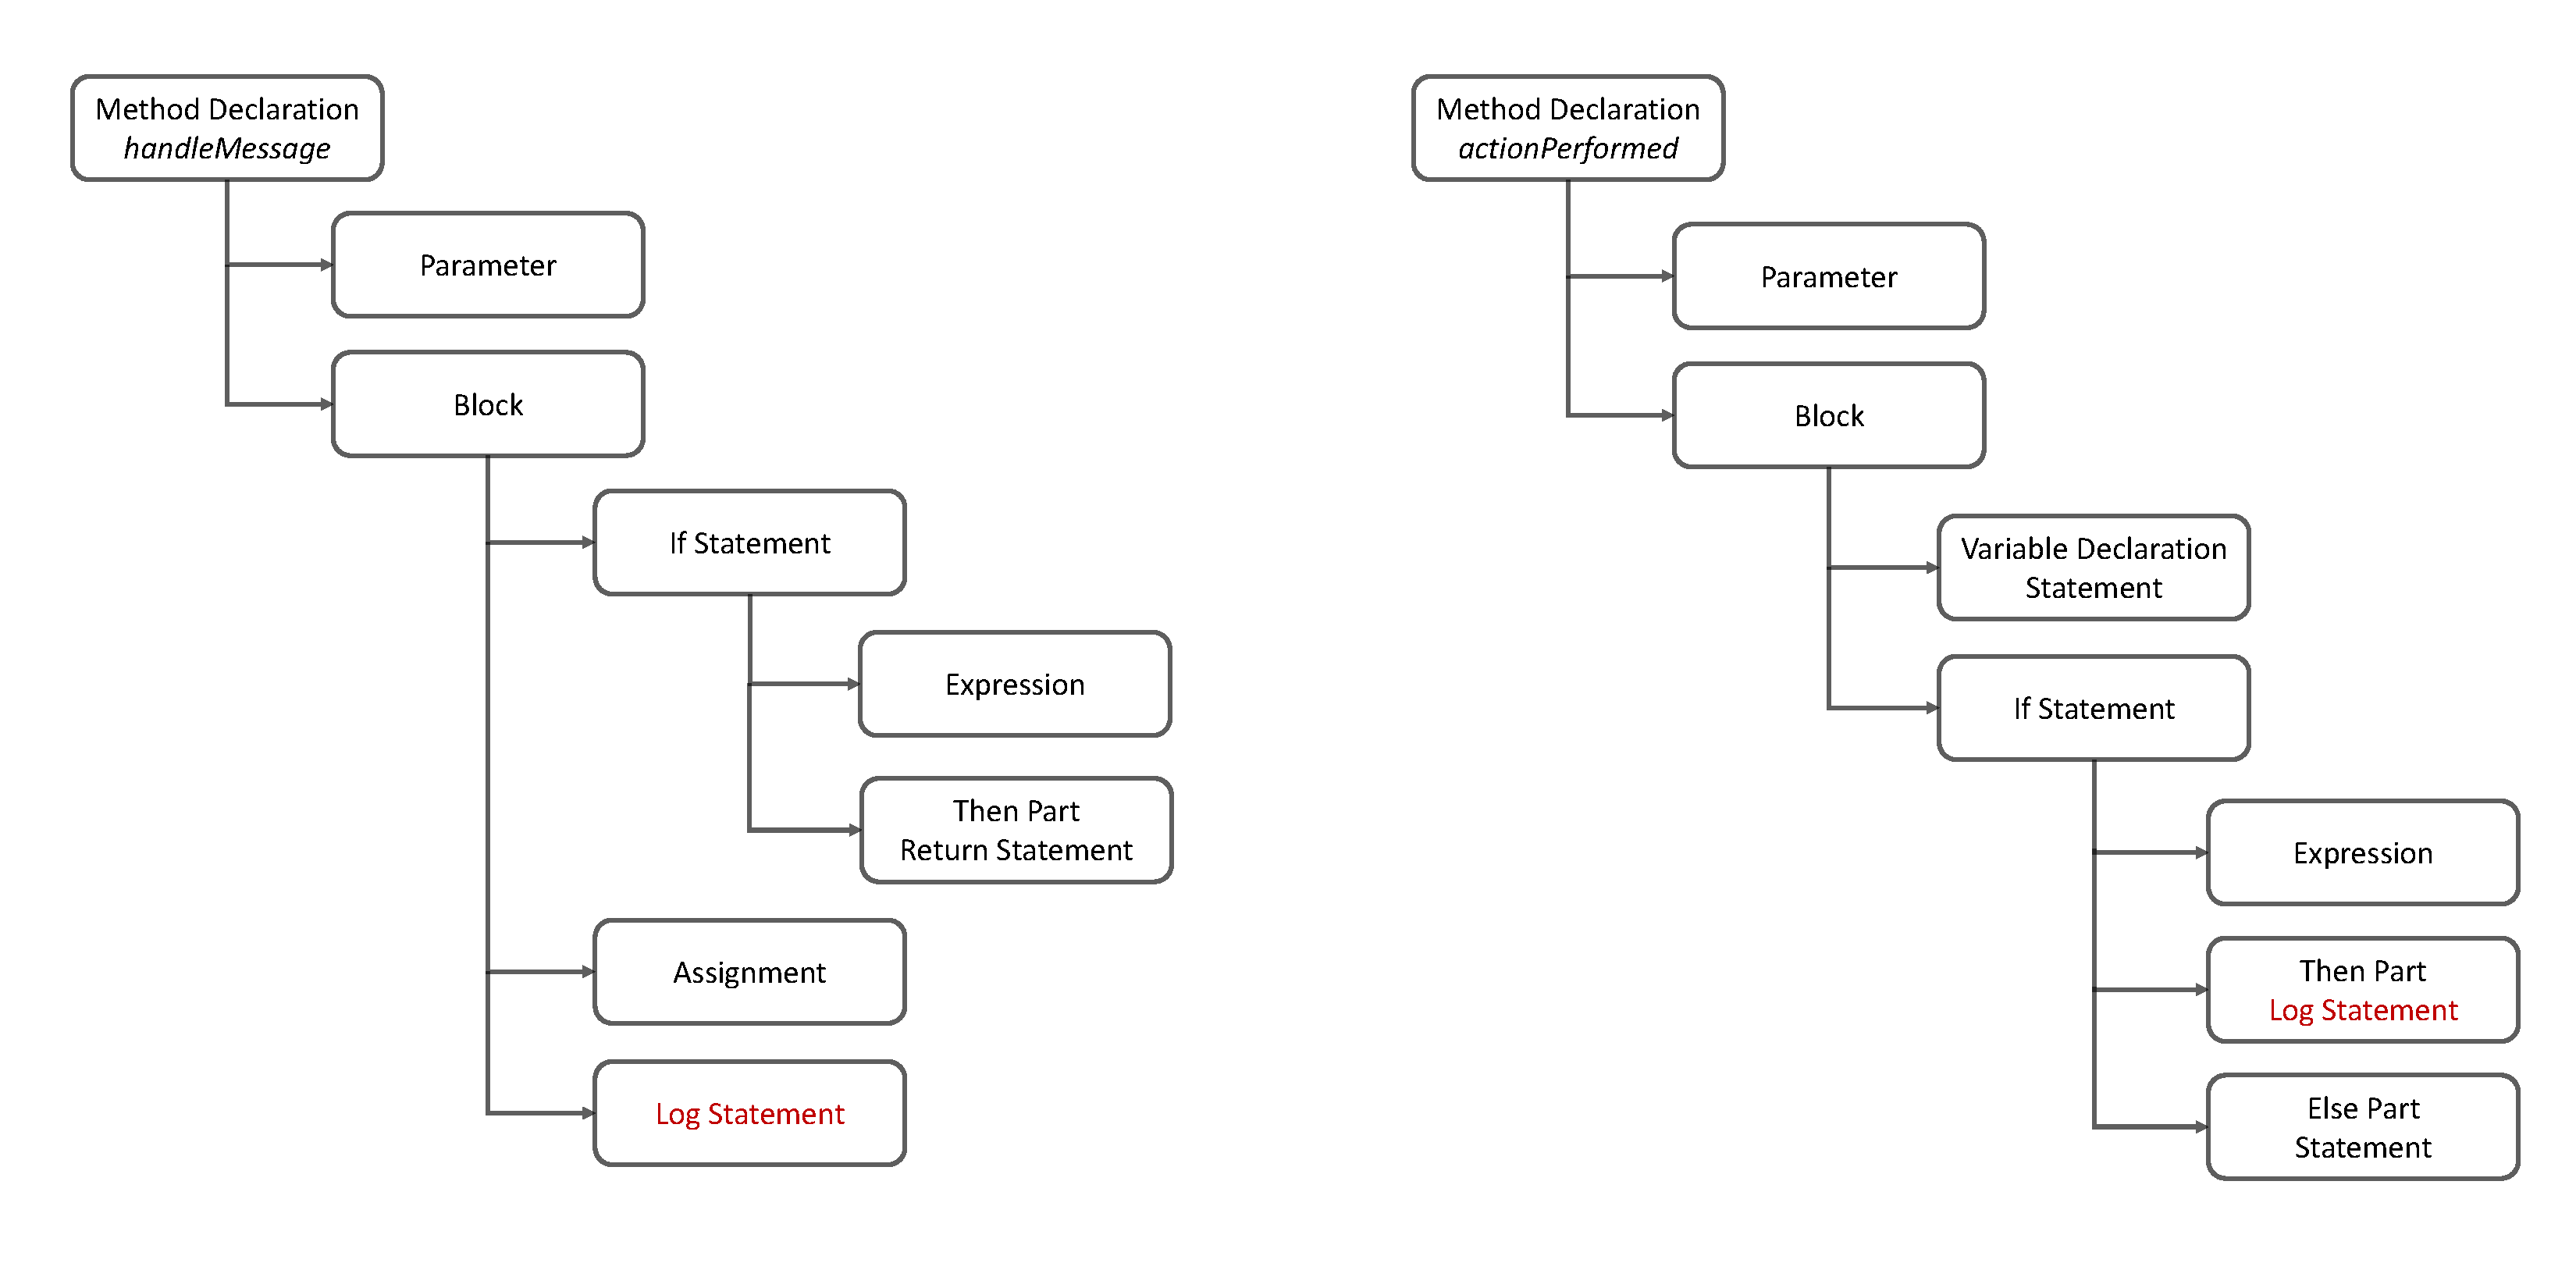
\includegraphics[width = \textwidth]{Drawing4/AST.pdf}
  \caption{Simple AST structure of the examples in Figures~\ref{ch3-ex1} and~\ref{ch3-ex2}.}
  \label{fig:ast}
\end{figure}

In the JDT framework, structural properties of each AST node can be used to obtain specific information about the Java element that it represents. These properties are stored in a map data structure that associates each property to its value; this data is divided into three types:
%property identifier???

\begin{itemize} [leftmargin=0.7in]
\item \textit{Simple structural properties:} These contain a simple value which has a primitive or simple type or a basic AST constant (e.g., identifier property of a name node whose value is a \code{String}).  For example, all the \textit{identifier} nodes in Figure~\ref{fig:java-example-ast} fall in this case; each references an instance of \code{String} representing the string that constitutes the identifier.
\item \textit{Child structural properties:} These involve situations where the value is a single AST node (e.g., name property of a method declaration node).  For example, the \textit{classDeclaration} node in Figure~\ref{fig:java-example-ast} has a single child that represents its name as an \textit{identifier} node.
\item \textit{Child list structural properties}: These involve situations where the value is a list of child nodes.  For example, the \textit{classDeclaration} node in Figure~\ref{fig:java-example-ast} can possess multiple \textit{modifier}s.
\end{itemize}

As an example, the ASTs of the log statements at line~4 of Figure~\ref{ch3-ex1} and Figure~\ref{ch3-ex2} can be represented respectively as:
\begin{itemize} [leftmargin=0.7in]
%\RW{These ASTs were messed up.  I fixed them according to what the code says.}
%\item \textit{expression(expression(Log), name(log), arguments(leftoperand(message), +, rightoperand(" is empty"), qualifier(Log), name(WARNING)))}
%\item \textit{expression(expression(Log), name(log), arguments(leftoperand(actionName),\\+, rightoperand("is an unknown action"), qualifier(Log), name(WARNING)))}
\item \textit{methodInvocation}(\\
\hspace*{1em}\textit{qualifiedName}(\code{Log}, \textit{identifier}(\code{log})),\\
\hspace*{1em}\textit{arguments}(\\
\hspace*{2em}\textit{qualifiedName}(\code{Log}, \mbox{\textit{identifier}(\code{WARNING})}),\\
\hspace*{2em}\textit{thisExpression}(),\\
\hspace*{2em}\textit{additionExpression}(\\
\hspace*{3em}\textit{methodInvocation}(\textit{identifier}(\code{getClassName}), \textit{arguments}()),\\
\hspace*{3em}\textit{stringLiteral}(\code{" should extend EditPlugin not EBPlugin since it has an empty "}),\\
\hspace*{3em}\textit{methodInvocation}(\textit{identifier}(\code{handleMessage}), \textit{arguments}()))))
\item \textit{methodInvocation}(\\
\hspace*{1em}\textit{qualifiedName}(\code{Log}, \textit{identifier}(\code{log})),\\
\hspace*{1em}\textit{arguments}(\\
\hspace*{2em}\textit{qualifiedName}(\code{Log}, \mbox{\textit{identifier}(\code{ERROR})}),\\
\hspace*{2em}\textit{thisExpression}(),\\
\hspace*{2em}\textit{additionExpression}(\\
\hspace*{3em}\textit{stringLiteral}(\code{"Unknown action: "}),\\
\hspace*{3em}\textit{identifier}(\code{actionName}))))
\end{itemize}

\section{First-order anti-unification}   \label{AU}

This section defines terms, substitutions, applying a substitution to a term, and instances of a term, as the requirements needed to describe first-order anti-unification.

\begin{defn}[First-Order Term]\label{def:term}
Given a set $V$ of variable symbols, a set $C$ of constant symbols, and sets $F_n$ of $n$-ary function symbols for all $n\ge1$, the set $T$ of \emph{first-order terms} is defined as the smallest set satisfying the recursion: (1) $V\subseteq T$; (2) $C\subseteq T$; and (3) for all $n$ first-order terms $t_1, \ldots, t_n$ and $n$-ary function symbol $f\in F_n$,  $f(t_1, \ldots, t_n) \in T$.
\end{defn}

Constant symbols can equivalently be considered 0-ary function symbols, with the appropriate adjustments to the above definition. For notational convenience, I use identifiers starting with a lowercase letter to represent function symbols (e.g., $f(a,b)$, $g(a,b)$) and constants (e.g., $a$, $b$), while variables are represented by identifiers starting with an uppercase letter (e.g., $X$, $Y$). The following are examples of a first-order term:
\begin{itemize} [leftmargin=0.7in]
\item $Y$
\item $a$
\item $f(X, c)$
\item $h(g(X, b),Y, g(a, Z))$
\end{itemize}
%A term is called grounded if it does not contain any variables (e.g., $f(a,b)}), and
Note that for any first-order term there is a unique, equivalent tree and vice versa: constant symbols and variable symbols are leaf nodes, while function symbols are non-leaf nodes; a function with given arguments is represented by a non-leaf node (representing the function symbol) with directed edges pointing to leaf nodes representing each argument.  For example:
\begin{itemize} [leftmargin=0.7in]
\item $Y$
\item $a$
\item \begin{tikzpicture}
\node(f) at (2,2) {$f$};
\node(X) at (1,1) {$X$};
\node(c) at (3,1) {$c$};
%
\draw[->](f) -- (X) {};
\draw[->](f) -- (c) {};
\end{tikzpicture}
%\item $X \leftarrow f \mapsto c$
\item \begin{tikzpicture}
\node(f) at (3,2) {$f$};
\node(g1) at (1,1) {$g$};
\node(Y) at (3,1) {$Y$};
\node(g2) at (5,1) {$g$};
\node(X) at (0,0) {$X$};
\node(b) at (2,0) {$b$};
\node(a) at (4,0) {$a$};
\node(Z) at (6,0) {$Z$};
%
\draw[->](f) -- (g1) {};
\draw[->](f) -- (Y) {};
\draw[->](f) -- (g2) {};
\draw[->](g1) -- (X) {};
\draw[->](g1) -- (b) {};
\draw[->](g2) -- (a) {};
\draw[->](g2) -- (Z) {};
\end{tikzpicture}
\end{itemize}

\begin{defn}[First-Order Substitution]\label{def:substitution}
A first-order substitution $\sigma$ is a mapping from variables $V$ to first-order terms $T$: $\sigma: V\mapsto T$. The notation $\{v_1 \mapsto t_1, \ldots, v_n \mapsto t_n\}$ is used to express a substitution of each of a set of variables $v_i$ by a corresponding first-order term $t_i$.
\end{defn}

\begin{defn}[Applying a First-Order Substitution]\label{def:substitution}
Applying a first-order substitution $\sigma = \{v_1 \mapsto t_1, \ldots, v_n \mapsto t_n\}$ to a first-order term $t$ results in the simultaneous replacement of all occurrences in $t$ of each variable $v_i$ by its corresponding first-order term $t_i$ as defined by the first-order substitution. This is denoted with the postfix expression $t\sigma$.
\end{defn}

As an example, applying the first-order substitution $\sigma = \{X \mapsto a, Y \mapsto b\}$
to the first-order term $f(X,Y)$ results in the replacement of all occurrences of the variable $X$ by the first-order term $a$ and all occurrences of the variable $Y$ by the first-order term $b$, and thus $f(X,Y)\sigma = f(a,b)$.

\begin{defn}[(First-Order) Instance]\label{def:instance}
For first-order terms $t_1$ and $t_2$, $t_2$ is called an \emph{instance} of $t_1$ if there exists a first-order substitution $\sigma$ such that $t_1\sigma = t_2$.
\end{defn}

%\begin{defn}[Unifier]\label{def:unifier}
%A unifier is a common instance of two given terms.
%\end{defn}

%Unification usually aims to create the \emph{most general unifier} (MGU); that is, $U$ is the MGU of two terms such that for all unifiers $U'$ there exists a substitution $\sigma$ such that $U\xrightarrow{\sigma}U'$. Unification aims to make a more concrete structure in essence, whereas what we need is a more generalized structure, which leads to the use of the dual of unification, called \emph{anti-unification}.

\begin{defn}[First-Order Anti-unifier]\label{def:generalization}
The term $t$ is a \emph{first-order anti-unifier} (or generalization) for first-order terms $t_1$ and $t_2$, if and only if there exist first-order substitutions $\sigma_1$ and $\sigma_2$ such that $t\sigma_1=t_1$ and $t\sigma_2=t_2$.
\end{defn}

A useful, first-order anti-unifier will contain only common pieces of the original terms, while the differences are abstracted away by replacing them with variable symbols. An anti-unifier for a pair of terms always exists since we can anti-unify any two terms by the term $X\in V$, i.e., a single variable. However, anti-unification usually aims to find the \emph{most specific anti-unifier} (MSA), that is, $t$ is the MSA of two first-order terms $t_1$ and $t_2$ if and only if there exists no anti-unifier $t'$ for $t_1$ and $t_2$ such that $t\sigma = t'$ for some first-order substitution $\sigma$.

As an example, an anti-unifier of the first-order terms $f(X,b)$ and $f(a,Y)$ is the first-order term $f(X,Y)$, containing common pieces of the two original, first-order terms. The variable $Y$ in the anti-unifier $f(X,Y)$ can be substituted by the first-order term $b$ to re-create $f(X,b)$ (with $\sigma_1 = \{Y\mapsto b\}$) and the variable $X$ in the anti-unifier can be substituted by the first-order term $a$ to re-create $f(a,Y)$
(with $\sigma_2 = \{X\mapsto a\}$), as depicted in Figure~\ref{fig:uni-anti-uni}.
%In addition, the unifier $f(a,b)$ of the two terms can be instantiated by applying the substitutions $\sigma_1'=X\xrightarrow{\sigma}a$ and $\sigma_2'=Y\xrightarrow{\sigma}b$ on the terms $f(X,b)$ and $f(a,Y)$, respectively.

\begin{figure} [t]
\centering\begin{tikzpicture}
\node(au) at (5,2) {\parbox{2cm}{\begin{center}\fbox{$f(X,Y)$}\\*[3pt]\text{anti-unifier}\end{center}}};
\node(left) at (2,0) {\fbox{\mbox{$f(X,b)$}}};
\node(right) at (8,0) {\fbox{\mbox{$g(a,Y)$}}};
\node(u) at (5,-2) {\parbox{2cm}{\begin{center}\fbox{$f(a,b)$}\\*[3pt]\text{unifier}\end{center}}};
%
\draw[->](au) -- (left) node[pos=0.5, above]{\mbox{\scriptsize $\sigma_1 = Y \mapsto b$\hspace*{2cm}}};
\draw[->](au) -- (right) node[pos=0.5, above]{\mbox{\hspace*{2.5cm}\scriptsize $\sigma_2 = X \mapsto a$}};
\draw[->](left) -- (u) node[pos=0.5, below]{\mbox{\scriptsize $\sigma_1' = X \mapsto a$\hspace*{2cm}}};
\draw[->](right) -- (u) node[pos=0.5, below]{\mbox{\hspace*{2.5cm}\scriptsize $\sigma_2' = Y \mapsto b$}};
\end{tikzpicture}
%  {\makecell[l]{\hspace{0.4cm}f(X,Y)\\\text{anti-unifier}}}
%  \arrow{dr}{\sigma_2 = X \mapsto a}
%  \arrow[->,swap]{dl}{\sigma_1 = Y \mapsto b} % <-- reflect the direction of the hook
%\\
%f(X,b)
% \arrow[->,swap]{dr}{\sigma_1' = X \mapsto a}
% %\arrow{dr}
%&&
%f(a, Y)
%  \arrow{dl}{\sigma_2' = Y \mapsto b}
%  \\
%&
%{\makecell[l]{f(a,b)\\\text{unifier}}}
%\end{tikzcd}
%\]
  \caption{Unification and anti-unification of the terms $f(X,b)$ and $f(a,Y)$.}
  \label{fig:uni-anti-uni}
\end{figure}

The MSA should preserve as much of the common pieces of both original first-order terms as possible; however, first-order anti-unification fails to capture complex commonalities, as first-order substitutions only replace first-order variables by first-order terms. That is, when two first-order terms differ in function symbols, first-order anti-unification fails to retain common details of the arguments in both terms. For example, the first-order anti-unifier of the terms $f(a,b)$ and $g(a,b)$ is $X$ as depicted in Figure~\ref{fig:first-anti-uni}.

\begin{figure}[t]
\centering\begin{tikzpicture}
\node(au) at (5,2) {\fbox{\mbox{$X$}}};
\node(left) at (2,0) {\fbox{\mbox{$f(a,b)$}}};
\node(right) at (8,0) {\fbox{\mbox{$g(a,b)$}}};
%
\draw[->](au) -- (left) node[pos=0.5, above]{\mbox{\scriptsize $\sigma_1 = X \mapsto f(a,b)$\hspace*{2cm}}};
\draw[->](au) -- (right) node[pos=0.5, above]{\mbox{\hspace*{2.5cm}\scriptsize $\sigma_2 = X \mapsto g(a,b)$}};
\end{tikzpicture}
\caption{First-order anti-unification of the terms $f(a,b)$ and $g(a,b)$.\label{fig:first-anti-uni}}
\end{figure}

\subsection{Higher-order anti-unification}
 
Higher-order anti-unification generalizes first-order anti-unification to permit function symbols to be substituted for certain variable symbols (functional ones, to be precise).  The needed formal definitions follow.

\begin{defn}[Higher-Order Term]\label{def:hterm}
Given a set $V$ of variable symbols, a set $C$ of constant symbols, sets $F_n$ of $n$-ary function symbols for all $n\ge1$, and sets $\mathbf{V}_m$ of $m$-ary functional variable symbols, the set $\hat{T}$ of \emph{higher-order terms} is defined as the smallest set satisfying the recursion: (1) $V\subseteq \hat{T}$; (2) $C\subseteq \hat{T}$; (3) for all $n$ higher-order terms $\hat{t}_1, \ldots, \hat{t}_n$ and $n$-ary function symbol $f\in F_n$,  $f(\hat{t}_1, \ldots, \hat{t}_n) \in \hat{T}$; and (4) for all $m$ higher-order terms $\hat{t}_1, \ldots, \hat{t}_m$ and $m$-ary functional variable symbol $F\in \mathbf{V}_m$,  $F(\hat{t}_1, \ldots, \hat{t}_n) \in \hat{T}$.
\end{defn}
 
Note that any first-order term on $V$, $C$, and $F_n$ will also be (a degenerate case of) a higher-order term on $V$, $C$, $F_n$, and $\mathbf{V}_m$ for all $\mathbf{V}_m$.
 
\begin{defn}[Higher-Order Substitution]\label{def:substitution}
A higher-order substitution $\hat{\sigma}$ is a mapping from variables $V$ to higher-order terms $\hat{T}$: $\sigma: V\mapsto T$ and, for all natural numbers $m\ge1$, from $m$-ary functional variables $\mathbf{V}_m$ to $m$-ary functional symbols $F_m$. The notation $\{\hat{v}_1 \mapsto \hat{t}_1, \ldots, \hat{v}_n \mapsto \hat{t}_n\}$ is used to express a substitution of each of a set of variables and functional variables $\hat{v}_i$ by a corresponding higher-order term $\hat{t}_i$ or functional symbols, where it is to be understood that a $m$-ary functional variable may only be substituted by a $m$-ary functional symbol and that a variable may only be substituted by a higher-order term.
\end{defn}

Note that a first-order substitution constitutes (a degenerate case of) a higher-order substitution.

\begin{defn}[Applying a Higher-Order Substitution]\label{def:substitution}
Applying a higher-order substitution $\hat{\sigma} = \{\hat{v}_1 \mapsto \hat{t}_1, \ldots, \hat{v}_n \mapsto \hat{t}_n\}$ to a higher-order term $\hat{t}$ results in the simultaneous replacement of all occurrences in $\hat{t}$ of each variable (respectively functional variable) $\hat{v}_i$ by its corresponding higher-order term (respectively functional variable) $\hat{v}_i$ as defined by the higher-order substitution. This is denoted with the postfix expression $\hat{t}\hat{\sigma}$.
\end{defn}

As an example, a higher-order anti-unifier of the terms $f(a,b)$ and $g(a,b)$ is $F(a,b)$ as depicted in Figure~\ref{fig:higher-anti-uni}.   For simplicity, I henceforth drop the adjectival phrases ``first-order'' and ``higher-order'' in cases where the intent is clear from the context.

\begin{figure}[t]
\centering\begin{tikzpicture}
\node(au) at (5,2) {\fbox{\mbox{$F(a,b)$}}};
\node(left) at (2,0) {\fbox{\mbox{$f(a,b)$}}};
\node(right) at (8,0) {\fbox{\mbox{$g(a,b)$}}};
%
\draw[->](au) -- (left) node[pos=0.5, above]{\mbox{\scriptsize $\hat{\sigma}_1 = \{F \mapsto f\}$\hspace*{2cm}}};
\draw[->](au) -- (right) node[pos=0.5, above]{\mbox{\hspace*{2.5cm}\scriptsize $\hat{\sigma}_2 = \{F \mapsto g\}$}};
\end{tikzpicture}
\caption{A higher-order anti-unification of the terms $f(a,b)$ and $g(a,b)$.\label{fig:higher-anti-uni}}
\end{figure}

Applying higher-order anti-unification could help to construct a structural generalization by maintaining the common pieces and abstracting the differences away using variables. However, it is not comprehensive enough to solve the problem as it does not consider background knowledge about AST structures, such as syntactically different but semantically equivalent structures, missing structures, and different ordering of arguments.
%In the following section, we will look at an extension of anti-unification, higher-order anti-unification modulo theories, and how it can sufficiently address the limitations of anti-unification in our context.

\section{Neutral elements and pumping}

Sometimes it is desirable to anti-unify terms with differing numbers of arguments.  To permit this, we can utilize the notion of pumping transformations and neutral elements.  For example, with the binary function symbols ``$+$'' and ``$\times$'' we have the neutral elements ``0'' and ``1'' respectively, so that $+(x, 0)=x$ and $\times(x, 1)=x$ (also $+(0, x)=x$ and $\times(1, x)=x$ because of the commutativity of these functions).  We can generalize this notion to the special $n$-ary function symbols $\id{pump}_n$ and to the special constant symbols $\nu_{\id{pump}_n}$ (each representing the neutral symbol for the indicated function), so that for any term $t$,
\begin{equation*}
\id{pump}_n(\nu_{\id{pump}_n}, \ldots, \nu_{\id{pump}_n}, t, \nu_{\id{pump}_n}, \ldots, \nu_{\id{pump}_n}) = t,
\end{equation*}
where there are exactly $n$ arguments to $\id{pump}_n(\cdot)$.  Furthermore, we define $\id{pump}_n(\cdot)$ to be perfectly commutative, so that $t$ may equivalently appear as any argument therein.

For simplicity of exposition, we use the label \NIL{} in place of both the functional symbols $\id{pump}_n$ and the neutral element of each of the functions thereby defined, as the precise meaning can be interpreted from the context.  Obviously, \NIL{} representing an $n$-ary functional symbol cannot be meaningfully anti-unified with \NIL{} representing an $n-k$-ary functional symbol---unless it is itself pumped.

\section{Higher-order anti-unification modulo equational theories}\label{HOAUMT}

%\begin{align}
%\sigma_1 = (W &\mapsto \text{ \textsf{\small WARNING}},\nonumber\\
%X &\mapsto \text{ \textit{methodCall}(\textit{simpleName}(\textsf{\small getClassName}), \textit{arguments}())},\nonumber\\
%Y &\mapsto \text{ \textsf{\small "should extend EditPlugin not EBPlugin since it has an empty "}},\nonumber\\
%Z &\mapsto \text{ \textit{methodCall}(\textit{simpleName}(\textsf{\small handleMessage}), \textit{arguments}())})\label{eq:theta1}\\
%\sigma_2 = (W &\mapsto \text{ \textsf{\small ERROR}},\nonumber\\
%X &\mapsto \text{ \NIL{}},\nonumber\\
%Y &\mapsto \text{ \textsf{\small "Unknown action: "}},\nonumber\\
%Z &\mapsto \text{ \textit{simpleName}(\textsf{\small actionName})})\label{eq:theta2}
%\end{align}
%
%%\item it can be mapped to our recursive definition of a term, where AST nodes and simple values may be viewed as function-symbols and constants, respectively
%
%\begin{figure}[p]
%\begin{small}
%\begin{tikzpicture}
%\node(a) at (4.25,10) {%
%\fbox{\parbox[b][][b]{3in}{%
%\text{\textit{methodCall}(}\\
%\text{\hspace*{1em}\textit{qualifiedName}(\textsf{\footnotesize Log}, \textit{simpleName}(\textsf{\footnotesize log})),}\\
%\text{\hspace*{1em}\textit{arguments}(}\\
%\text{\hspace*{2em}\textit{qualifiedName}(\textsf{\footnotesize Log}, \textit{simpleName}(\textit{W})),}\\
%\text{\hspace*{2em}\textit{thisExpression}(),}\\
%\text{\hspace*{2em}\textit{additionExpression}(\textit{X}, \textit{stringLiteral}(\textit{Y}), \textit{Z})))}}}%
%};
%\node(b) at (0,0) {%
%\fbox{\parbox[t][][b]{3.1in}{%
%\text{\textit{methodCall}(}\\
%\text{\hspace*{1em}\textit{qualifiedName}(\textsf{\footnotesize Log}, \textit{simpleName}(\textsf{\footnotesize log})),}\\
%\text{\hspace*{1em}\textit{arguments}(}\\
%\text{\hspace*{2em}\textit{qualifiedName}(\textsf{\footnotesize Log},}\\ \text{\hspace*{3em}\mbox{\textit{simpleName}(\textsf{\footnotesize WARNING})}),}\\
%\text{\hspace*{2em}\textit{thisExpression}(),}\\
%\text{\hspace*{2em}\textit{additionExpression}(}\\
%\text{\hspace*{3em}\textit{methodCall}(\textit{simpleName}(\textsf{\footnotesize getClassName}),}\\ \text{\hspace*{4em}\textit{arguments}()),}\\
%\text{\hspace*{3em}\textit{stringLiteral}(\textsf{\footnotesize " should extend ... "}),}\\
%\text{\hspace*{3em}\textit{methodCall}(\textit{simpleName}(\textsf{\footnotesize handleMessage}),}\\ \text{\hspace*{4em}\textit{arguments}()))))}}}%
%};
%\node(c) at (8.5,0.7) {%
%\fbox{\parbox[t][][b]{2.55in}{%
%\text{\textit{methodCall}(}\\
%\text{\hspace*{1em}\textit{qualifiedName}(\textsf{\footnotesize Log}, \textit{simpleName}(\textsf{\footnotesize log})),}\\
%\text{\hspace*{1em}\textit{arguments}(}\\
%\text{\hspace*{2em}\textit{qualifiedName}(\textsf{\footnotesize Log},}\\ \text{\hspace*{3em}\mbox{\textit{simpleName}(\textsf{\footnotesize ERROR})}),}\\
%\text{\hspace*{2em}\textit{thisExpression}(),}\\
%\text{\hspace*{2em}\textit{additionExpression}(}\\
%\text{\hspace*{3em}\textit{stringLiteral}(\textsf{\footnotesize "Unknown action: "}),}\\
%\text{\hspace*{3em}\textit{simpleName}(\textsf{\footnotesize actionName}))))}}}%
%};
%
%\draw[->](a) -- (b) node[pos=0.5,above]{$\sigma_1\qquad$};
%\draw[->](a) -- (c) node[pos=0.5,above]{$\qquad\sigma_2$};
%\end{tikzpicture}
%\end{small}
%\caption{The anti-unification of the AUASTs of the logging calls in Examples 1 and 2.\label{fig:logging-anti}}
%\end{figure}
%%The AUASTs of log Method Invocation nodes from the Java classes in Figure~\ref{ch3-ex1} and Figure~\ref{ch3-ex2}.
%
%Applying higher-order anti-unification on AUAST structures could help to construct a structural generalization by maintaining the common pieces and abstracting the differences away using variables. However, it is not comprehensive enough to solve our problem as it does not consider background knowledge about AST structures, such as syntactically different but semantically relevant structures, missing structures, and different ordering of arguments. In the following section, we will look at an extension of anti-unification, higher-order anti-unification modulo theories, and how it can sufficiently address the limitations of anti-unification in our context.

%anti-unification cannot incorporate any background knowledge such as sematic knowledge required to solve our problem, and we should apply an extended form of anti-unification, called higher-order anti-unification modulo theories, where a set of equivalence equations is defined to incorporate semantic knowledge of structural equivalences supported by the Java language specification. An equivalence equation $=_E$ determines which terms are considered equal, and the set of equivalence equations must be applied on higher-order extended structures to allow the anti-unification of AST structures that are not identical but are semantically equivalent.
In higher-order anti-unification modulo (equational) theories, a set of equational theories, which treat different structures as equivalent, is defined to incorporate background knowledge. Each equational theory $=_E$ determines which terms are considered equal and a set of these equations can be applied on higher-order extended structures to determine structural equivalences. For example, we have introduced an equational theory $=_E$, such that $f(t,u) =_E f(u,t)$ to indicate that the ordering of arguments does not matter in our context.

% nil restriction!!!!
The notion of pumping from the previous section is equivalent to defining an equational theory $=_{\id{pump}}$ such that 
\begin{gather*}
\id{pump}_n(\nu_{\id{pump}_n}, \ldots, \nu_{\id{pump}_n}, t, \nu_{\id{pump}_n}, \ldots, \nu_{\id{pump}_n})\\
=_{\id{pump}} \id{pump}_{n-1}(\nu_{\id{pump}_{n-1}}, \ldots, \nu_{\id{pump}_{n-1}}, t, \nu_{\id{pump}_{n-1}}, \ldots, \nu_{\id{pump}_{n-1}})\\
=_{\id{pump}} \ldots\\
=_{\id{pump}} \id{pump}_1(t)\\
=_{\id{pump}} t
\end{gather*}
Or equivalently:
\begin{gather*}
\NIL{}(\NIL{}, \ldots, \NIL{}, t, \NIL{}, \ldots, \NIL{})\\
=_{\id{pump}} \NIL{}(\NIL{}, \ldots, \NIL{}, t, \NIL{}, \ldots, \NIL{})\\
=_{\id{pump}} \ldots\\
=_{\id{pump}} \NIL{}(t)\\
=_{\id{pump}} t
\end{gather*}
For simplicity, I refer to this as the \NIL{}-theory. 

For example, we can anti-unify the two terms $b$ and $f(a,b)$ through the application of the \NIL{}-theory by creating the term $\NIL{}(\NIL{},b)$---which is $=_{\id{pump}}$ to $b$---and anti-unifying $\NIL{}(\NIL{},b)$ with $f(a,b)$ as depicted in Figure~\ref{fig:anti-nil} to arrive at $F(X, b)$.

%restrictions???

% to introduce an equivalence equation =E for the NIL structure
% it should be modified
% should it be different?
\begin{figure}[t]
\centering\begin{tikzpicture}
\node(au) at (5,2) {\fbox{\mbox{$F(X,b)$}}};
\node(left) at (2,0) {\fbox{\mbox{$f(a,b)$}}};
\node(right) at (8,0) {\fbox{\mbox{$\NIL{}(\NIL{},b) =_{\id{pump}}  b$}}};
%
\draw[->](au) -- (left) node[pos=0.5, above]{\mbox{\scriptsize $\sigma_1 = ( F \mapsto f, X \mapsto a)$\hspace*{3cm}}};
\draw[->](au) -- (right) node[pos=0.5, above]{\mbox{\hspace*{3.5cm}\scriptsize $\sigma_2 = ( F \mapsto \NIL{}, X \mapsto \NIL{})$}};
\end{tikzpicture}
\caption{Higher-order anti-unification modulo theories of the terms $f(a, b)$ and $b$.\label{fig:anti-nil}}
\end{figure}


We have also defined a set of equational theories to incorporate semantic knowledge of structural equivalences supported by the \name{Java} language specification, as it provides various syntactic ways to define semantically equivalent structures. 
%These theories should be applied on higher-order extended structures to anti-unify AST structures that are not identical but are semantically equivalent. 
For example, consider \code{for}- and \code{while}-statements that are two kinds of looping structure in \name{Java}: they have different syntax but cover the same concept. To be able to anti-unify these structures meaningfully, we need an equational theory that can equate any \code{for}-loop---\code{for(}$\id{inits}$\code{; }$\id{test}$\code{; }$\id{updates}$\code/){...}/---to an equivalent \code{while}-loop---$\id{inits}$\code{; while(}$\id{test}$\code/) {...; /$\id{updates}$\code/;}/.  


Most simply, we could treat the two loops as functions with differing arguments, defining an equivalence equation $=_{\id{loops}}$ that allows their direct anti-unification. We would then utilize the \NIL{}-theory to handle the varying number of arguments as the \code{for}-loop has three arguments whereas the \code{while}-loop only has one. Using the \NIL{}-theory we can create the structure \code{while}(\NIL{}(\NIL{}, \NIL{}), \textit{lessThanExpression}(\code{i}, \code{10}), \NIL{}(\NIL{}, \NIL{})) that is $=_{\id{loops}}$ to \code{while}(\textit{lessThanExpression}(\code{i}, \code{10})) and construct the anti-unifier, $V_0$($V_1$($V_2$, $V_3$), \textit{lessThanExpression}(\code{i}, \code{10}), $V_4$($V_5$($V_2$))), as depicted in Figure~\ref{fig:for-while}.

\begin{figure}[t]
\centering\begin{tikzpicture}
\node(au) at (5,5) {\fbox{\parbox{2in}{$V_0(V_1(V_2,V_3),$\\$\text{\quad\textit{lessThanExpression}(\textsf{\small i}, \textsf{\small 10})}$,\\ \mbox{$\quad V_4(V_5(V_2)))$}}}};
%
\node(left) at (0,0) {\fbox{\parbox{2.75in}{%
\textsf{\small for}(\textit{initializer}(\textsf{\small i}, \textsf{\small 0}),\\\mbox{\quad\textit{lessThanExpression}}(\textsf{\small i}, \textsf{\small 10}),\\ \mbox{\quad\textit{updater}}(\textit{postIncrementExpression}(\textsf{\small i})))}}};
%
\node(right) at (10,0) {\fbox{\parbox{2in}{%
\textsf{\small while}(\NIL{}(\NIL{}, \NIL{}),\\ \mbox{\quad\textit{lessThanExpression}}(\textsf{\small i}, \textsf{\small 10}),\\ \mbox{\quad\NIL{}}(\NIL{}(\NIL{})))}}};
%
\draw[->](au) -- (right) node[pos=0.5, above]{$\qquad\sigma_2$};
%
\draw[->](au) -- (left) node[pos=0.5, above]{$\sigma_1\qquad$};
\end{tikzpicture}
\caption[Complex anti-unification of two structures demonstrating a \protect\NIL{}-theory.]{Anti-unification of the structures \code{for}(\textit{initializer}(\code{i}, \code{0}), \mbox{\textit{lessThanExpression}(\code{i}, \code{10}),} \textit{updater}(\textit{postIncrementExpression}(\code{i}))) and \code{while}(\NIL{}(\NIL{}, \NIL{}), \mbox{\textit{lessThanExpression}(\code{i}, \code{10}),} \NIL{}(\NIL{}, \NIL{})). The substitutions are defined as follows: $\sigma_1 = (V_0 \mapsto \text{ \textsf{\small for}}, V_1 \mapsto \text{ \textit{initializer}}, V_2 \mapsto \text{ \textsf{\small i}}, V_3 \mapsto 0, V_4 \mapsto \text{ \textit{updater}}, V_5 \mapsto \text{ \textit{postIncrementExpression}})$; and $\sigma_2 = (V_0 \mapsto \text{ \textsf{\small while}}, V_1 \mapsto \text{ \NIL{}}, V_2 \mapsto \text{ \NIL{}}, V_3 \mapsto \text{ \NIL{}}, V_4 \mapsto \text{ \NIL{}}, V_5 \mapsto \text{ \NIL{}})$\label{fig:for-while}}
\end{figure}
% higher-order extension and the equational theories
% provide a better example

In practice, this is more usefully accomplished by converting the \code{for}-loop to the equivalent \code{while}-loop and anti-unifying the result directly, which can find correspondences between the initialization expression and equivalent assignment statements prior to the \code{while}-loop, and between the update expression and equivalent statements, typically at the end of the block in the \code{while}-loop.

\subsection{Loss of uniqueness}
Defining complex substitutions in higher-order anti-unification modulo theories results in losing the uniqueness of the MSA. For example, consider the terms $f_1(g(a,e))$ and $f_2(g(a,b),$\linebreak$g(d,e))$. As described in Figure~\ref{fig:multipleMSA}, two MSAs exist for these terms: we can anti-unify $g(a,e)$ and $g(a,b)$ to create the anti-unifier $g(a,X)$ and anti-unify $g(d,e)$ with the \NIL{} structure to create the anti-unifier $G(Y,Z)$; or we can anti-unify $g(a,e)$ and $g(d,e)$ to create the anti-unifier $g(X,e)$ and anti-unify $g(a,b)$ with the \NIL{} structure to create the anti-unifier $F(Y,Z)$.

\begin{figure}[t]
\centering\begin{tikzpicture}
\node(au) at (5,2) {\fbox{\mbox{$F(g(X,e),G(Y,Z))$}}};
\node(left) at (2,0) {\fbox{\mbox{$f_2(g(a,b), g(d,e))$}}};
\node(right) at (8,0) {\fbox{\mbox{$f(g(a,e))$}}};
%
\draw[->](au) -- (left) node[pos=0.5, above]{\mbox{\scriptsize $\sigma_1 = \{F\mapsto f_2, X\mapsto d, G\mapsto g, Y\mapsto a, Z\mapsto b\}$\hspace*{6cm}}};
\draw[->](au) -- (right) node[pos=0.5, above]{\mbox{\hspace*{7cm}\scriptsize $\sigma_2 = \{F\mapsto f_1, X\mapsto a, G\mapsto \NIL{}, Y\mapsto \NIL{}, Z\mapsto \NIL{}\}$}};
\end{tikzpicture}
\vspace*{1em}

\centering\begin{tikzpicture}
\node(au) at (5,2) {\fbox{\mbox{$F(g(a,X),G(Y,Z))$}}};
\node(left) at (2,0) {\fbox{\mbox{$f_2(g(a,b), g(d,e))$}}};
\node(right) at (8,0) {\fbox{\mbox{$f_1(g(a,e))$}}};
%
\draw[->](au) -- (left) node[pos=0.5, above]{\mbox{\scriptsize $\sigma_1 = \{F\mapsto f_1, X\mapsto b, G\mapsto g, Y\mapsto d, Z\mapsto e\}$\hspace*{6cm}}};
\draw[->](au) -- (right) node[pos=0.5, above]{\mbox{\hspace*{7cm}\scriptsize $\sigma_2 = \{F\mapsto f_2, X\mapsto e, G\mapsto\NIL{}, Y\mapsto\NIL{}, Z\mapsto\NIL{})$}};
\end{tikzpicture}
\caption[Ambiguous higher-order anti-unification modulo theories of two terms.]{Ambiguous higher-order anti-unification modulo theories of the terms $f_2(g(a,b), g(d,e))$
and $f_1(g(a,e))$, creating multiple MSAs.}
  \label{fig:multipleMSA}
\end{figure}


Despite having multiple potential MSAs, I need to determine one single MSA that is the most appropriate in my context. However, the complexity of finding an optimal MSA is undecidable in general \cite{2008:fse:cottrell} since an infinite number of possible substitutions can be applied to variables in a term. Therefore, I need to use an approximation technique to construct one of the best MSAs that can sufficiently solve the problem.
% reason, infinite number??? ever variable???
%Our goal is to find an MSA that is an approximation of the best fit to our application


\section{The Jigsaw Tool}\label{Jigsaw}

\name{Jigsaw} is a plug-in to the Eclipse integrated development environment (IDE), which was developed by \citet{2008:fse:cottrell} to support small-scale source code reuse via structural correspondence. A small-scale reuse task can be divided into two phases. The first phase involves the developer identifying a source code snippet that implements functionality that is missing within a target system. The second phase involves integrating the source code snippet within the target system.
\name{Jigsaw} supports the small scale reuse task by identifying structural correspondences between the code snippet and the context into which the code should be pasted, in order to suggest to developers what parts already exist within the target system, what parts are missing, and what parts need to be modified to fit into the context. In summary, the \name{Jigsaw} tool determines the structural correspondences between two \name{Java} source code fragments through the application of higher-order anti-unification modulo equational theories such that one fragment can be integrated to the other one for small-scale code reuse.

%To perform a reuse task, developers mostly copy and paste the reused code snippet and then fit it to the hole of the target context by performing some modifications.

In general, the proposed approach by \citeauthor{2008:fse:cottrell} proceeds in three steps. First, it generates an augmented form of AST, called a \emph{correspondence AST} (CAST), where each node holds a list of candidate correspondence connections, each implicitly representing an anti-unifier. To find candidate correspondences amongst the CASTs of the original system and the target system, it uses a similarity measure that relies on syntactic similarity along with simple knowledge of semantic equivalences supported the Java language specifications. Although the CAST structure may represent many anti-unifiers, they used a greedy selection algorithm to select the best fit for each node via thresholding in order to approximate the optimal generalization. That is, the correspondence connections with a similarity value below a threshold are removed. Second, when there is more than one candidate correspondence connection for a node, the developer is prompted to resolve the conflict by selecting the best fit for his functionality. Third, the best correspondences are used to semi-automatically perform the integration task by replacing the references to variables in the original system by the references to variables in the target system. The Jigsaw tool is a proof-of-concept implementation of this approach.

Underlying the Jigsaw tool is the Jigsaw framework for determining likely structural correspondences between two ASTs; I simply refer to ``Jigsaw'' henceforth to intend the Jigsaw framework.
The Jigsaw similarity function returns a value in $[0, 1]$ where zero indicates complete lack of similarity and one indicates perfect similarity. In general, this function returns a value above zero if the compared nodes are of identical type, and thus it returns a similarity of 0 for the nodes of different types. However, it uses several heuristics to improve the utility of the similarity measurement by defining an arbitrary value for the nodes that are syntactically different but are semantically relevant. For example, the similarity between names of AST nodes is measured using a normalized computation based on the length of the longest common substring. The comparison of the \code{int} and \code{long} nodes is another example, where an arbitrary value of 0.5 is defined as the similarity, since they are not of syntactically identical types but have a semantic equivalence. This function also detects the correspondence between \code{for}-, \code{enhanced-for}-, \code{while}-, and \code{do}-loop statements; and \code{if} and \code{switch} conditional statements.


As I intend to construct a structural generalization from ASTs of two logged methods via structural correspondence, it could be helpful to use the first phase of the proposed approach to find candidate correspondences using the similarity measure. However, the second phase does not help determine the best correspondences needed in my context, as the CAST generated via thresholding neither resolves the conflicts that occur in constructing one single anti-unifier automatically, nor prevents the anti-unification of log statement nodes with any other nodes. There, the Jigsaw similarity function does not enable us to measure how similar are the usages of log statements inside methods. In addition, as the problem of this study is different, the integration phase of the approach is not related to my work. Instead, I should develop an algorithm to construct a detailed view of the generalization describing the structural commonalities and differences between logged methods. However, the CAST structure does not suffice to construct an anti-unifier: it does not allow the insertion of \emph{structural variables} in place of nodes in the tree structure, and thus an extended form is required. In the following chapters, I will discuss my approach to create a structural generalization and its implementation by means of the higher-order anti-unification modulo theories.
\section{Clustering}  \label{ch3-clustering}
Clustering is the classification of a collection of data objects into meaningful groups (clusters) \cite{jain1999data}. The goal of clustering is to find groups of objects such that the objects in one cluster will be similar to one another and dissimilar from the objects in other clusters. The greater the similarity amongst the objects within a cluster and the greater the dissimilarity between the objects from various clusters are, the more distinct the clusters would be \cite{}.  In general, there are two major types of clustering:
%\cite[][Chapter 8]{tan2013data} ????

\begin{itemize} [leftmargin=.4in]
\item \emph{Partitional clustering:} which aims to divide the data objects into non-overlapping clusters such that each data object is in utterly one cluster.
\item \emph{Hierarchical clustering:} which aims to generate a set of nested clusters organized as a hierarchical structure. Each cluster in the structure is the union of its subclusters, and the cluster at the top contains all the the data objects.
\end{itemize}

The following will introduce two popular techniques used to perform clustering on a data set:

% supervised-unsupervisod?
%dendogram?
\subsubsection{K-means clustering algorithm}
% indicate Lines ??? initial centroids???
This algorithm is a partitional clustering approach that attempts to find a certain number of clusters, which are represented by centriod (the center of a cluster). In this algorithm, ${K}$ is the number of the resulting clusters that should be specified. Each cluster is associated with a centroid  which is mostly the average of all the
data objects within the cluster or the most representative object of a
cluster. The basic K-means clustering technique is described using the Algorithm~\ref{alg:k-means}. This algorithm repeatedly assigns each data object to a cluster with the nearest centroid and computes the new clusters centroids accordingly. This process terminates when it reaches a state in which no objects are moving from one cluster to another, and thus, the centroids don't change.
%strength?
The K-means clustering algorithm is not a good fit to this study, as it requires to specify the number of resulting clusters, which is not reasonable to my problem context. %??
% representative object?

%Each object is assigned to a centroid is a cluster. The centroid of each cluster is then updated based on the objects assigned to the cluster.  repeatedly perform the assignment and update opertaions util the centroids do not change.

\begin{algorithm}
\caption{Basic K-means clustering algorithm.} \label{alg:k-means}
\begin{algorithmic}[1]
\State Select K data objects as initial centroids.
\Repeat
\State Assigning each object to its closes centroid.
\State Update the centroid of each cluster.
\Until Centroids remain the same.
\end{algorithmic}
\end{algorithm}



\subsubsection{Agglomerative hierarchical clustering algorithm}
%LINES???
%dendogram?
The agglomerative hierarchical clustering algorithm produce a nested grouping of clusters, with single point clusters at the bottom and an all-inclusive cluster at the top \cite{karypis1999chameleon}. Agglomerative hierarchical clustering is one of the main stream clustering methods \cite{day1984efficient} that has applications in document retrieval \cite{voorhees1986implementing} and information retrieval from a search engine query log \cite{beeferman2000agglomerative}. Algorithm~\ref{alg:agglomerative} describes the basic agglomerative hierarchical clustering appraoch. It starts with the individual objects as singleton clusters, and successively, merges the two closest clusters until only one all inclusive cluster remains. In general, hierarchical clustering algorithms work implicitly or explicitly with the $n \times n$ similarity matrix such that an element in row $i$ and column $j$ represents the similarity between the $i$th and the $j$th clusters \cite{karypis1999chameleon}.
% dandogram ???
%update???


\begin{algorithm}
\caption{Basic agglomerative hierarchical clustering algorithm.} \label{alg:agglomerative}
\begin{algorithmic}[1]
\State Start with singleton clusters.
\State Compute the similarity matrix.
\Repeat
\State Merge the closest cluster pair.
\State Update the similarity matrix by computing the similarity between new cluster and all remaining clusters.
\Until Only one cluster remains.
\end{algorithmic}
\end{algorithm}




%until a pre-determined number of clusters is obtained or the similarity between the closest clusters becomes below a pre-determined threshold value.

%[Rasmussen, 1992] \RW{Put into bibtex}?????

There are various versions of agglomerative hierarchical algorithms that mainly differ in how they update the similarity between clusters. There are various methods to measure the similarity between clusters, such as single linkage, complete linkage, average linkage, and centroids \cite{}. In the single linkage method, the similarity is measured by the similarity of the closest pair of data points of two clusters. In the complete linkage method, the similarity is computed by the similarity of the farthest pair of data points of two clusters. In the average linkage method, the similarity is measured by the average of all pairwise similarities between data points of two clusters. In the centroids methods, each cluster is represented by a centroid, and the similarity between two clusters is measured by the similarity of the clusters' centroids. However, I need to develop a modified version of the basic agglomerative hierarchical clustering algorithm to address my problem context. In the modified version, the merge and update operations should be terminated when the similarity between the closest clusters becomes below a pre-determined threshold value. Furthermore, I need to develop a measure of the similarity between the clusters based on the similarity between their anti-unifiers. In Chapter~\ref{clustering}, I describe how I modified the basic hierarchical algorithm to my problem context.

%in our application, each cluster is composed of one AUAST, and the similarity between two clusters is measured by the similarity between the clusters' AUASTs, which is the ratio of the number of common pieces over the total number of pieces of their anti-unifier.


%optimal clusters
%. Partitional clustering try to classify a data set into $k$ clusters such that the partition optimizes a pre-determined criterion \cite{karypis1999chameleon}. The most popular partitional clustering algorithm is $k$-means, which repeatedly assigns each data point to a cluster with the nearest centroid and computes the new cluster centroids accordingly until a pre-determined number of clusters is obtained \cite{bouguettaya2015efficient}.

\section{Summary}  \label{summary}
I described abstract syntax trees (ASTs) as a standard syntactic representation of source code. Every AST can also be represented in a functional format (and vice versa) which constitute the standard theoretical concept of terms. I presented Eclipse JDT as a concrete framework that can be used to manipulate ASTs of a source code written in the \name{Java} programming language.

I demonstrated how the theoretical framework of anti-unification can be used as a technique to construct a common generalization of two given terms, and hence of two ASTs.  First-order anti-unification permits terms to be replaced with variables and vice versa, but it is limited in that low-level commonality can be discarded due to high-level differences.  Higher-order anti-unification overcomes this by permitting substitution relative to function symbols as well as terms. A further extension allows for insertion and deletion by declaring equivalence with the \NIL{} structure, as well as other arbitrary equational theories to embed knowledge of semantic equivalence.  Unfortunately, this approach of higher-order anti-unification modulo theories leads to ambiguity and the potential for an infinite number of possible substitutions for every structural variable.  To make use of that technique despite its weaknesses, we must apply an approximation technique to select amongst the best MSAs in order to reach a solution that is reasonable in practice. I also introduced Jigsaw, an existing framework for determining structural correspondences between ASTs and why it does not adequately address my problem.  To address my problem, I describe in subsequent chapters how I extended the Jigsaw framework. Furthermore, I introduced a hierarchical clustering algorithm that can be applied to classify logged methods into different categories.

%approximated or modified? 
\addtocontents{toc}{\protect\addvspace{10pt}}
\chapter{Background: Eclipse JDT and Jigsaw}\label{background2}

In order to construct structural generalizations describing the commonalities and differences between logged Java methods (LJMs), we need a concrete framework for constructing and manipulating abstract syntax trees (ASTs).  The Eclipse integrated development environment provides such a framework in its Java Development Tools (JDT) component.  The details of our implementation will depend on certain details of Eclipse JDT, so we describe those in Section~\ref{JDT}.

A framework exists for determining structural correspondences between ASTs, called Jigsaw \cite{2008:fse:cottrell}.  We build atop that work in order to create our anti-unifiers. We describe Jigsaw in Section~\ref{Jigsaw}.

\section{Eclipse JDT}\label{JDT}

The Eclipse Java Development Tools (JDT) framework provides APIs to access and manipulate Java source code via ASTs. An AST represents Java source code in a tree form, where the typed nodes represent instances of certain syntactic structures from the Java programming language.  Each node type (in general) takes a set of child nodes, also typed and with certain constraints on their properties.  Groups of children are named on the basis of the conceptual purpose of those groups; optional groups can be empty, which we can represent with the \NIL{} element. Thus, any Java source code can be represented as a tree of AST nodes. For example, the simple AST structure of two sample logged Java classes in Figures~\ref{ch3-ex1} an~\ref{ch3-ex2} is shown in Figure~\ref{fig:ast}

\begin{figure}[p]
\def\baselinestretch{1}
\begin{lstlisting}
public abstract class EBPlugin extends EditPlugin implements EBComponent {
    private Boolean seenWarning;

    protected EBPlugin() {
    }

    public void handleMessage(EBMessage message) {
        if(seenWarning) return;
        seenWarning = true;
        Log.log(Log.WARNING, this, getClassName() + " should extend EditPlugin not EBPlugin since it has an empty " + handleMessage());
    }
}
\end{lstlisting}
\caption{A Java class that uses a logging call. This will be referred to as Example 1.\label{ch3-ex1}}
\end{figure}

\begin{figure}[p]
\def\baselinestretch{1}
\begin{lstlisting}
public static class Wrapper implements ActionListener {
    private ActionContext context;
    private String actionName;

    public Wrapper(ActionContext context,  String actionName) {
        this.context = context;
        this.actionName = actionName;
    }

    public void actionPerformed(ActionEvent evt) {
        EditAction action = context.getAction(actionName);
        if(action == null) {
            Log.log(Log.ERROR, this, "Unknown action: " + actionName);
        }
        else
            context.invokeAction(evt, action);
    }
}
\end{lstlisting}
\caption{A Java class that uses a logging call. This will be referred to as Example 2.\label{ch3-ex2}}
\end{figure}

\begin{figure} [p]
  \centering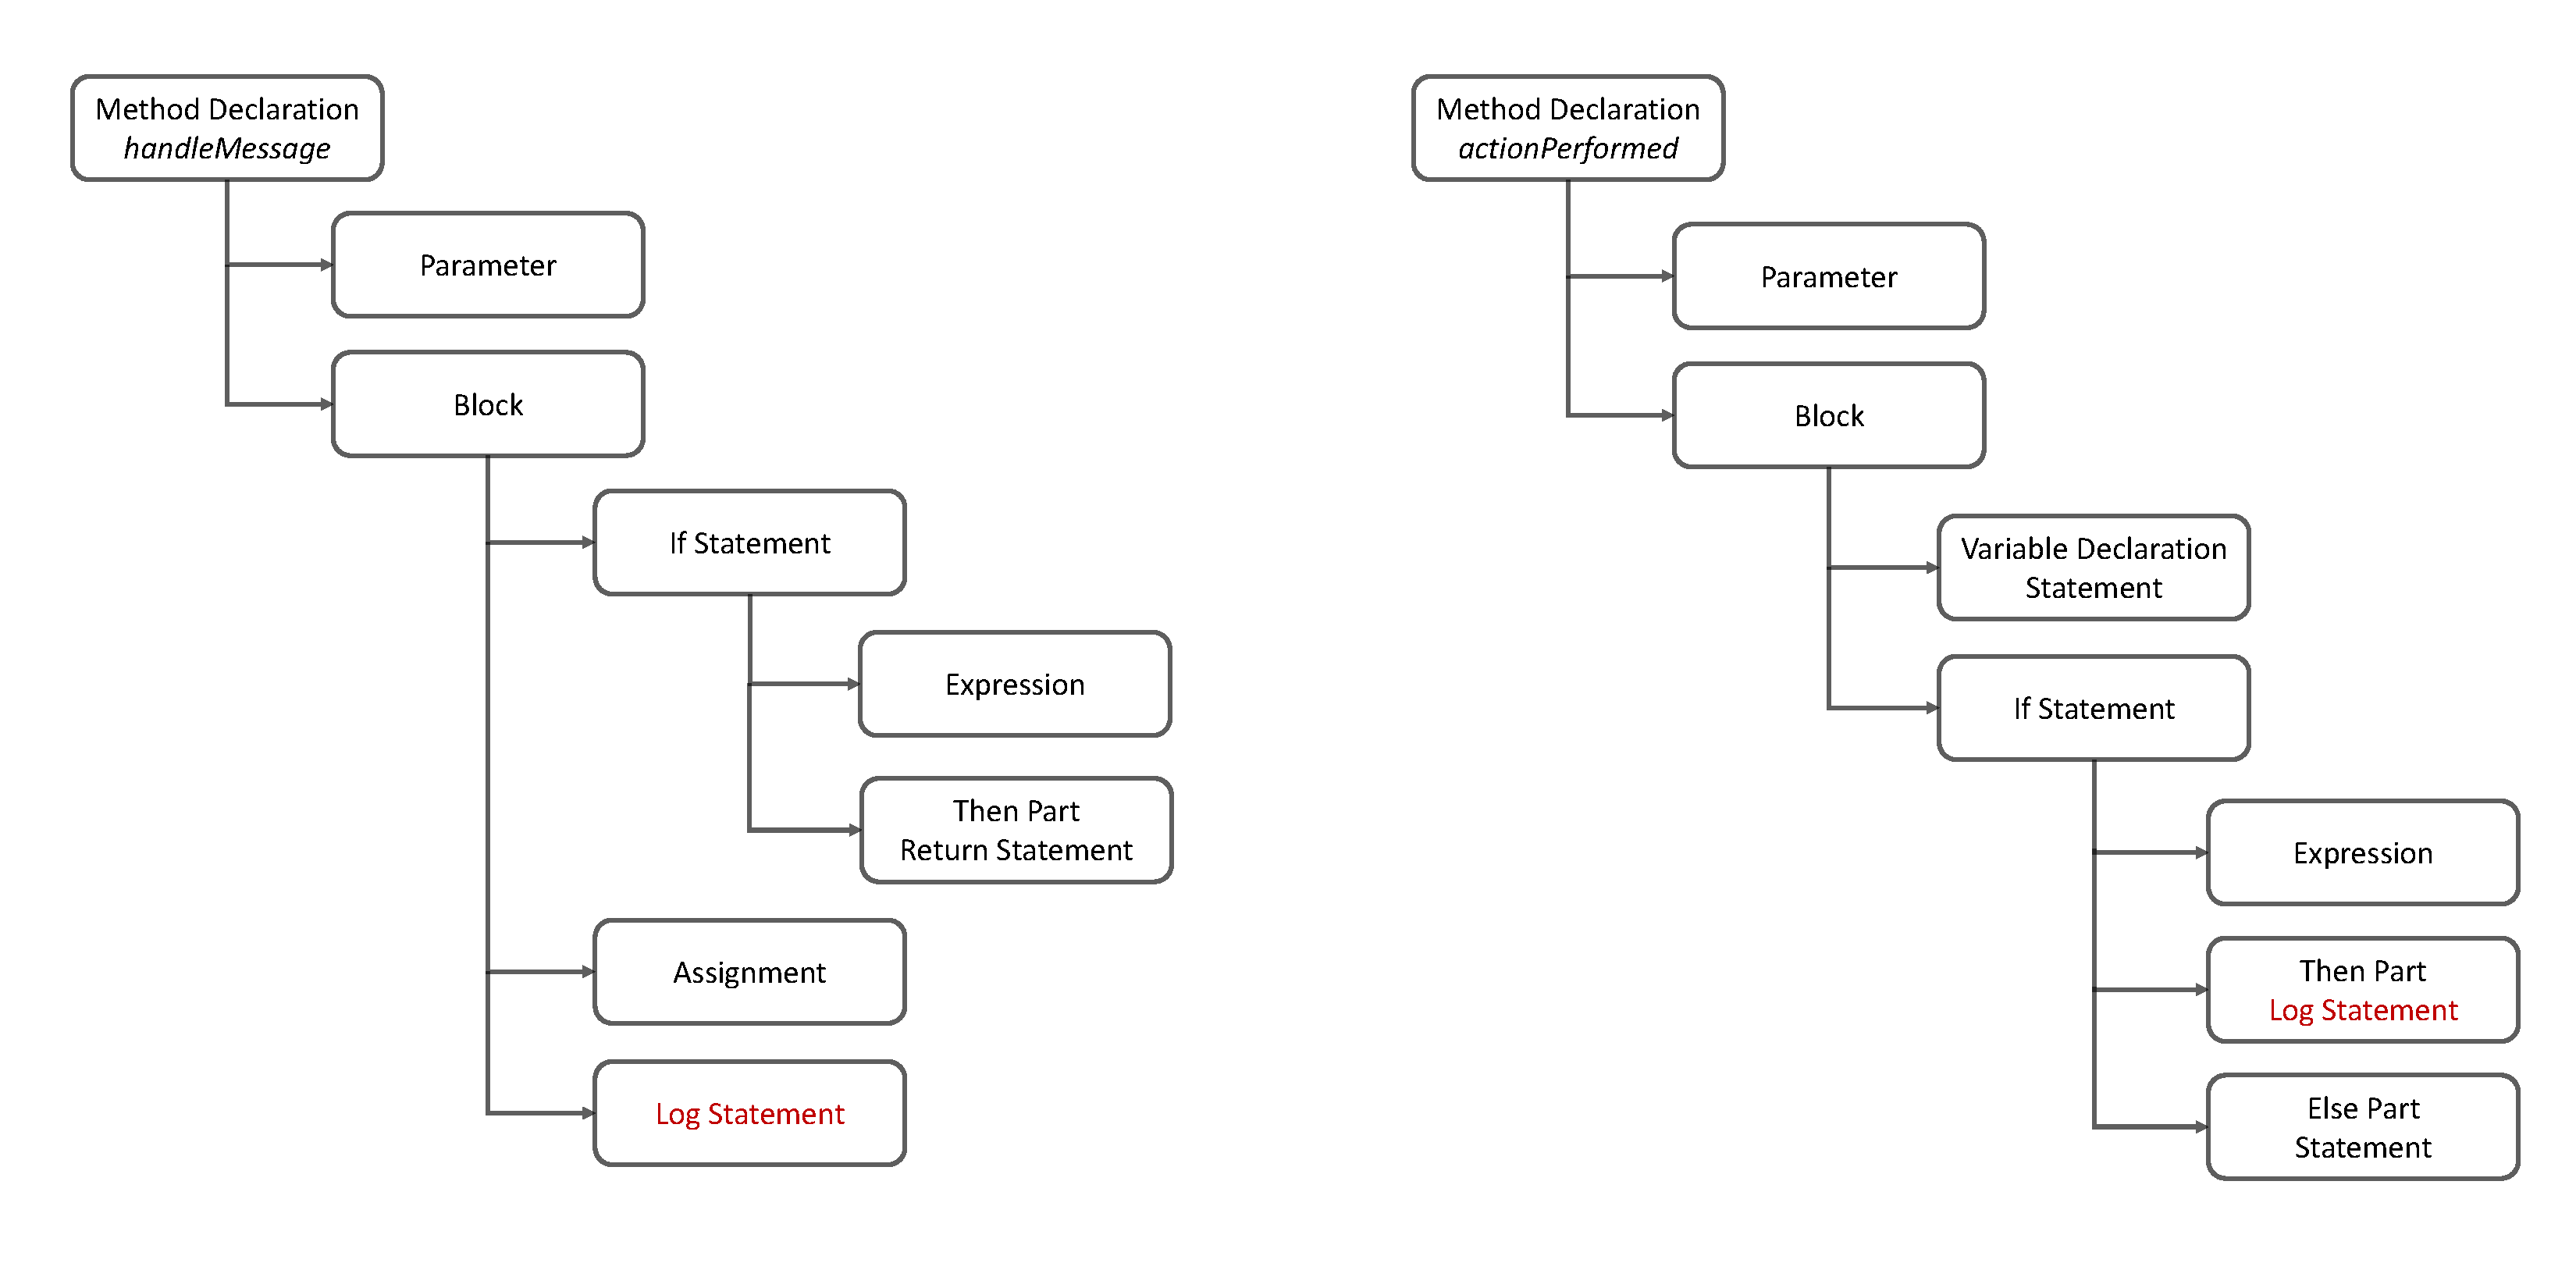
\includegraphics[width = \textwidth]{Drawing4/AST.pdf}
  \caption{Simple AST structure of examples in Figures~\ref{ch3-ex1} and~\ref{ch3-ex2}.}
  \label{fig:ast}
\end{figure}

In the JDT framework, structural properties of each AST node can be used to obtain specific information of the Java element that it represents. These properties are stored in a map data structure that associates each property to its value; this data is divided into three types:
\begin{itemize} [leftmargin=0.7in]
\item \textit{Simple structural properties:} These contain a simple value which has a primitive or simple type or a basic AST constant (e.g., identifier property of a name node whose value is a String).  For example, all the \textit{Identifier} nodes in Figure~\ref{fig:java-example-ast} fall in this case; each references an instance of \code{String} representing the string that constitutes the identifier.
\item \textit{Child structural properties:} These involve situations where the value is a single AST node (e.g., name property of a method declaration node).  For example, the \textit{ClassDeclaration} node in Figure~\ref{fig:java-example-ast} has a single child that represents its name as an \textit{Identifier} node; this would be a child structural property.
\item \textit{Child list structural properties}: These involve situations where the value is a list of child nodes.  For example, the \textit{ClassDeclaration} node in Figure~\ref{fig:java-example-ast} can possess multiple \textit{Modifier}s; these are recorded in the \textit{ClassDeclaration} as a child list structural property.
\end{itemize}

As an example, the ASTs of the logging calls at line~10 of Figure~\ref{ch3-ex1} and line~13 of Figure~\ref{ch3-ex2} can be represented respectively as:
\begin{itemize} [leftmargin=0.7in]
%\RW{These ASTs were messed up.  I fixed them according to what the code says.}
%\item \textit{expression(expression(Log), name(log), arguments(leftoperand(message), +, rightoperand(" is empty"), qualifier(Log), name(WARNING)))}
%\item \textit{expression(expression(Log), name(log), arguments(leftoperand(actionName),\\+, rightoperand("is an unknown action"), qualifier(Log), name(WARNING)))}
\item \textit{MethodCall}(\\
\hspace*{1em}\textit{QualifiedName}(\code{Log}, \textit{Identifier}(\code{log})),\\
\hspace*{1em}\textit{Arguments}(\\
\hspace*{2em}\textit{QualifiedName}(\code{Log}, \mbox{\textit{Identifier}(\code{WARNING})}),\\
\hspace*{2em}\textit{ThisExpression}(),\\
\hspace*{2em}\textit{AdditionExpression}(\\
\hspace*{3em}\textit{MethodInvocation}(\textit{Identifier}(\code{getClassName}), \textit{Arguments}()),\\
\hspace*{3em}\textit{StringLiteral}(\code{" should extend EditPlugin not EBPlugin since it has an empty "}),\\
\hspace*{3em}\textit{MethodInvocation}(\textit{Identifier}(\code{handleMessage}), \textit{Arguments}()))))\\
\item \textit{MethodInvocation}(\\
\hspace*{1em}\textit{QualifiedName}(\code{Log}, \textit{Identifier}(\code{log})),\\
\hspace*{1em}\textit{Arguments}(\\
\hspace*{2em}\textit{QualifiedName}(\code{Log}, \mbox{\textit{Identifier}(\code{ERROR})}),\\
\hspace*{2em}\textit{ThisExpression}(),\\
\hspace*{2em}\textit{AdditionExpression}(\\
\hspace*{3em}\textit{StringLiteral}(\code{"Unknown action: "}),\\
\hspace*{3em}\textit{Identifier}(\code{actionName}))))\\
\end{itemize}

\section{The Jigsaw framework}\label{Jigsaw}
The Jigsaw tool was developed by \citet{2008:fse:cottrell} to determine the structural correspondences between two Java source code fragments through the application of higher-order anti-unification modulo equational theories such that one fragment can be integrated to the other one for small-scale code reuse. Jigsaw could help determine potential candidate structural correspondences between AST nodes of logged Java classes by producing an augmented form of AST, called a \emph{correspondence AST} (CAST), where each node holds a list of candidate correspondence connections between the two structures, each implicitly representing an anti-unifier. Jigsaw also provides a measure of structural similarity to indicate how similar the nodes involved in each correspondence connection are. The Jigsaw similarity function relies on structural correspondence along with simple knowledge of semantic equivalences supported by the Java language specification. It returns a value in $[0, 1]$ where zero indicates complete lack of similarity and one indicates perfect similarity. In addition, several semantical heuristics are used to improve the accuracy of similarity measurement by allowing the comparison of AST nodes that are not syntactically identical but are semantically related to each other.

For example, the similarity between names of AST nodes is measured using a normalized computation based on the length of the longest common substring. The comparison of \code{int} and \code{long} types is another example, where an arbitrary value of 0.5 is defined as the similarity value as they are not syntactically identical but are semantically related. In addition, the Jigsaw framework also detects the structural correspondence between  \code{for}-, enhanced-\code{for}-, \code{while}-, and \code{do}-loop statements; and \code{if} and \code{switch} conditional statements. As an example, Figure~\ref{fig:meth-ast-1} shows the structural correspondence connections created by Jigsaw between the AST nodes of Examples 1 and 2 along with the similarity value for each correspondence connection.

\begin{figure} [H]
  \centering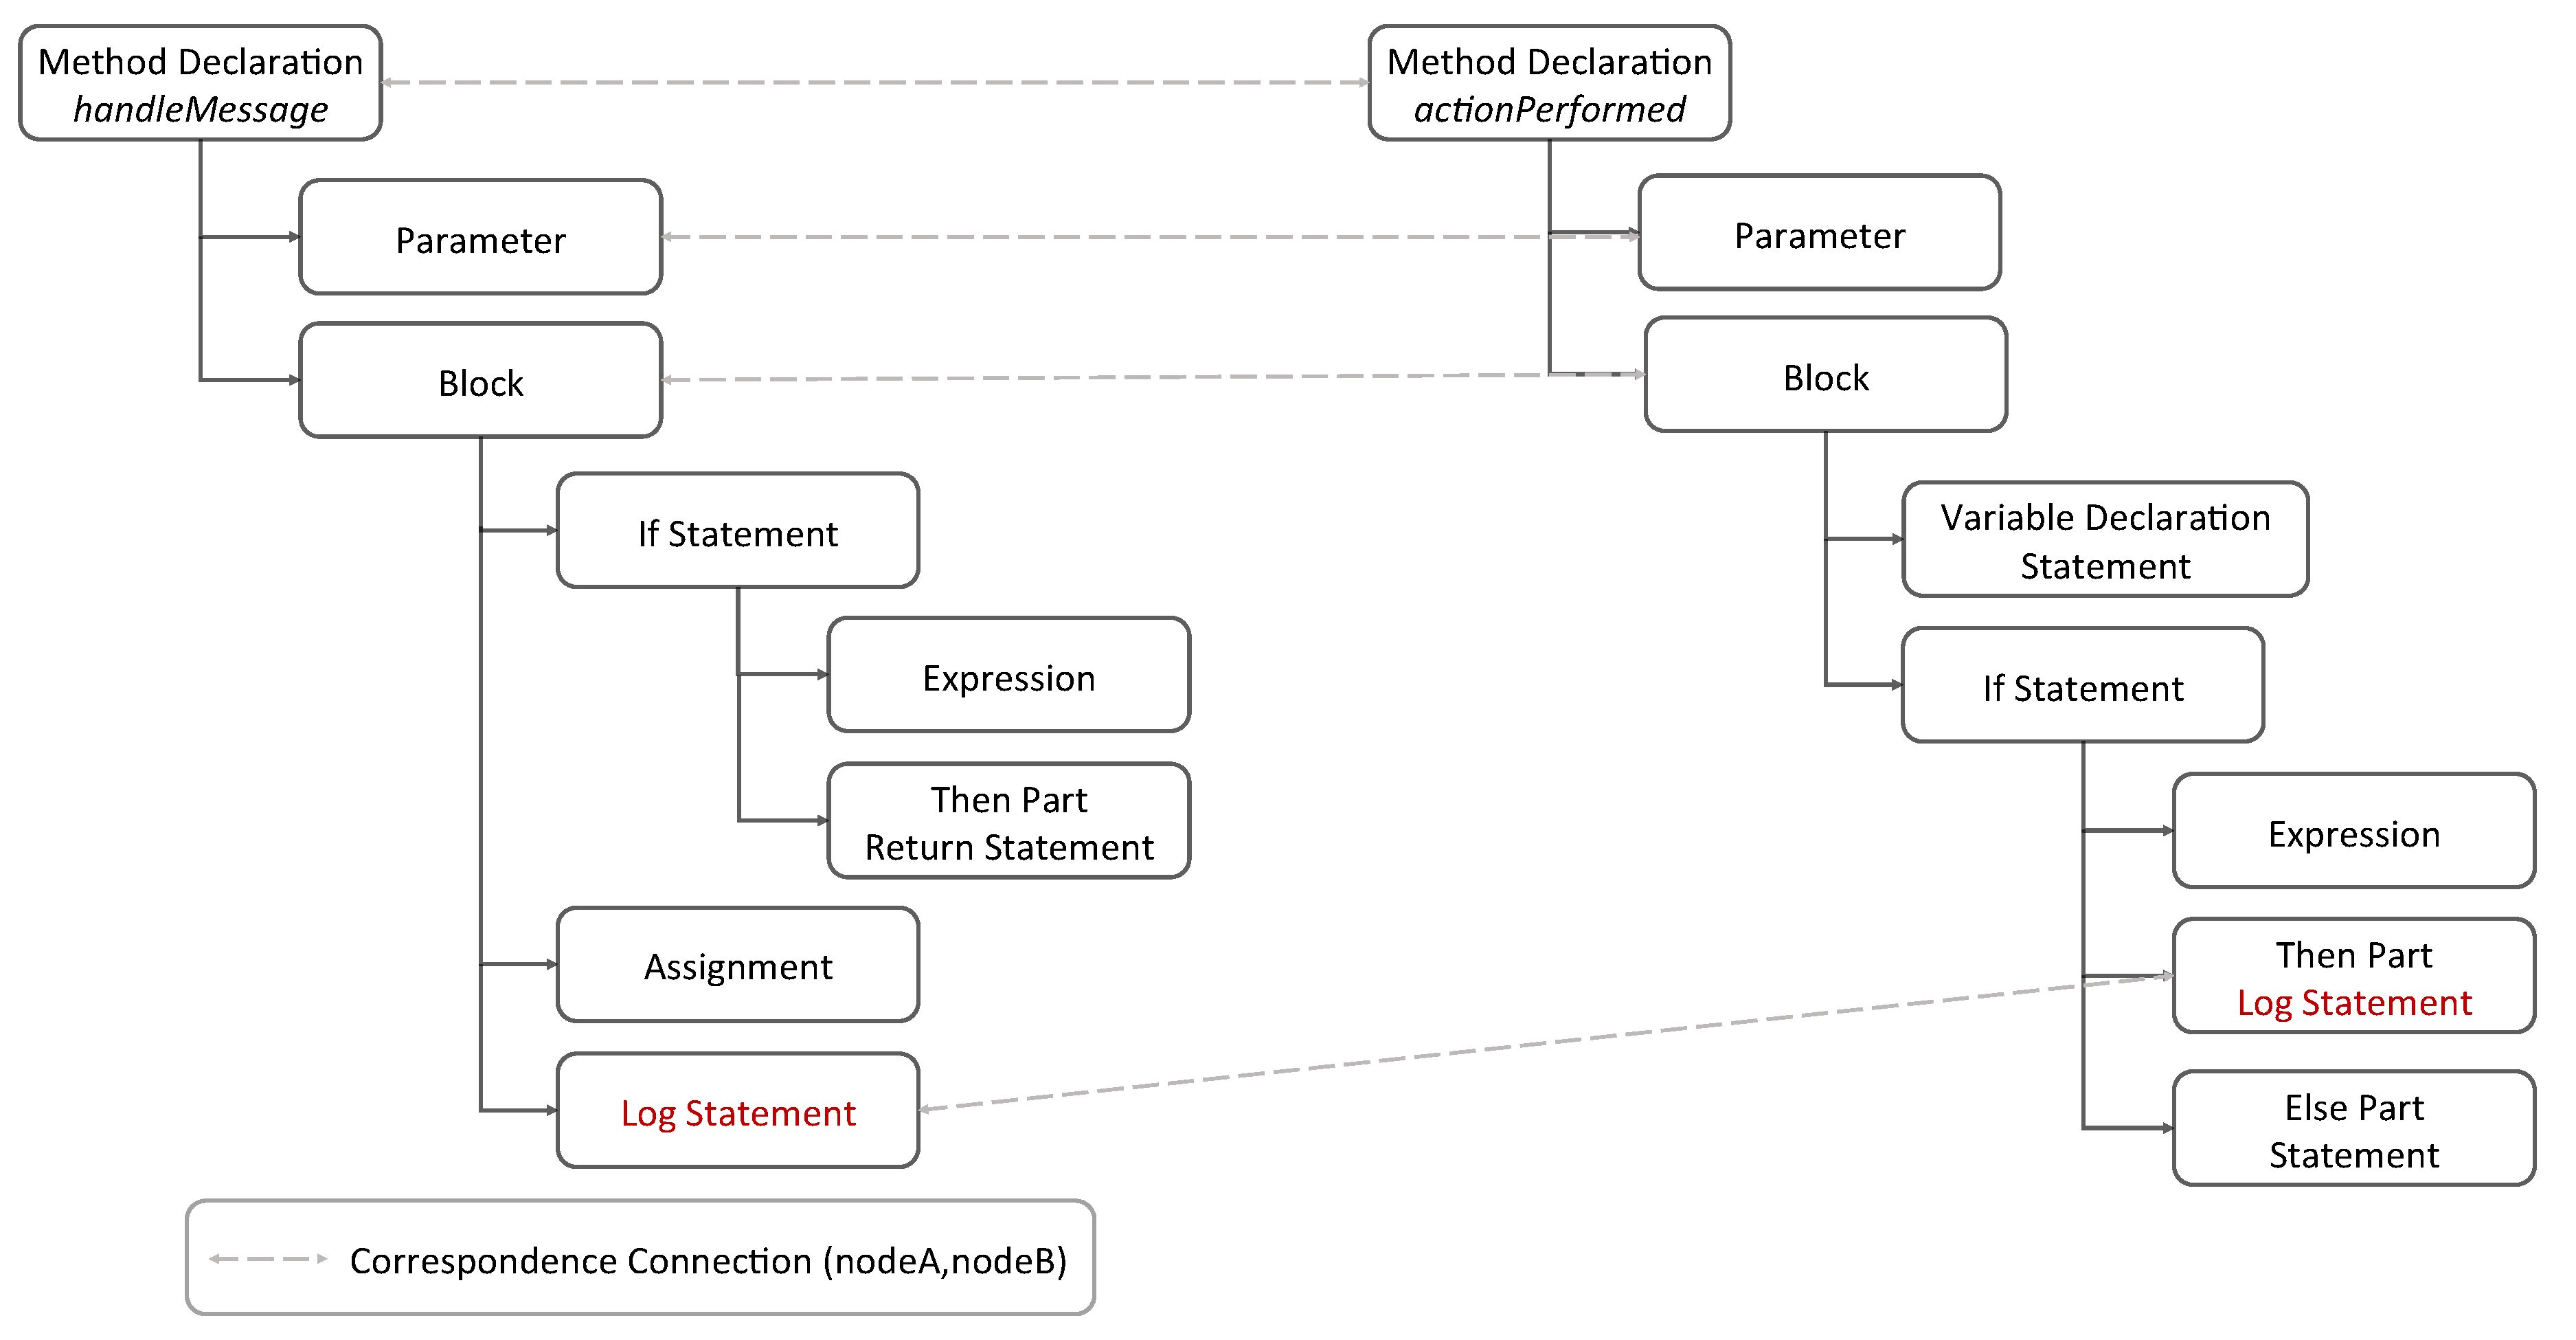
\includegraphics [width = \textwidth]{Drawing4/FirstCorr.pdf}
  \caption{Simple CAST structure of examples in Figures~\ref{ch3-ex1} and~\ref{ch3-ex2}. The links between AST nodes indicate structural correspondence connections created by the Jigsaw framework along with the similarity value.}
  \label{fig:meth-ast-1}
\end{figure}

However, the Jigsaw tool does not suffice to construct an anti-unifier that is the best fit to our application. In addition, the Jigsaw similarity function does not measure the similarity of two logged Java classes with a focus on logging calls, which is needed in our context. To address these issues, we should develop a greedy selection algorithm to approximate the best anti-unifier by determining the best correspondence for each node. In the following chapter, we will discuss our approach to construct structural generalizations and our implementation by means of the higher-order anti-unification modulo theories and the Jigsaw framework.

\section{Summary}  \label{summary}
\RW{Redo}
\addtocontents{toc}{\protect\addvspace{10pt}}
\chapter{Constructing Structural Generalizations} \label{ch4} \label{methodology}

In Chapter~\ref{background}, I provided background information on higher-order anti-unification modulo theories, a theoretical framework that can be used to construct a generalization from two given ASTs. I also presented the framework proposed by \citet{2008:fse:cottrell} to construct the CAST structure, where each node holds a list of candidate structural correspondences in Chapter~\ref{background2}. I next extended the CAST structure to AUAST that would allow the creation of an anti-unifier. I now consider how these frameworks could help me (1)~to construct an approximation of the best anti-unifier to my problem from the AUASTs of two logged methods with special attention to log statements and (2)~to develop a similarity measure between the two structures, which can provide us with useful information for clustering a set of logged methods in a later phase. The constructed anti-unifier can be viewed as a generalization that represents the structural commonalities and differences between the two logged methods.


%I also described how Jigsaw applies this framework on ASTs of a pair of \name{Java} methods to determine candidate structural correspondences.

%To this end, first we should create an extended form of AST, called AUAST (Anti-unifier AST) that allows the insertion of variables in place of any node in the tree, which is a requirement for HOAUMT (see Section~\ref{AUAST}).
%1) generates all possible candidate correspondence connections between the two AUASTs using the Jigsaw framework (line~1) (see Section~\ref{meth-CAST});

To approximate the best anti-unifier for my problem, I should develop a greedy selection algorithm that determines the best correspondence for each node. My approach contains a sequence of 2 actions to find the best correspondences between two AUASTs: (1) it applies two constraints to prevent the anti-unification of log statement nodes with any other nodes; and (2) it determines the best correspondence for each AUAST node with the highest similarity and then removes the other correspondence connections involving those nodes (Section~\ref{best-corr}). However, to construct an anti-unifier, a further step should be taken, which is the anti-unification of each AUAST node with its best correspondence (Section~\ref{meth-antiUnifier}). Furthermore, I developed an algorithm to measure similarity between the usage of logging calls in methods based on the selected correspondences (Section~\ref{meth-similarity}). An overview of the proposed anti-unification approach is shown in Figure~\ref{fig:meth_overview}.





%computed the ratio of the number of common elements over the total number of elements of the anti-unifier to measure similarity between two AUASTs (see Section~\ref{meth-similarity}).
%I computed the ratio of the number of common elements over the total number of elements of the anti-unifier to measure similarity between two AUASTs (see Section~\ref{meth-similarity}).
%(Section ~\ref{meth-constraints})
%through anti-unifying their structural properties



\begin{figure} [H]
  \centering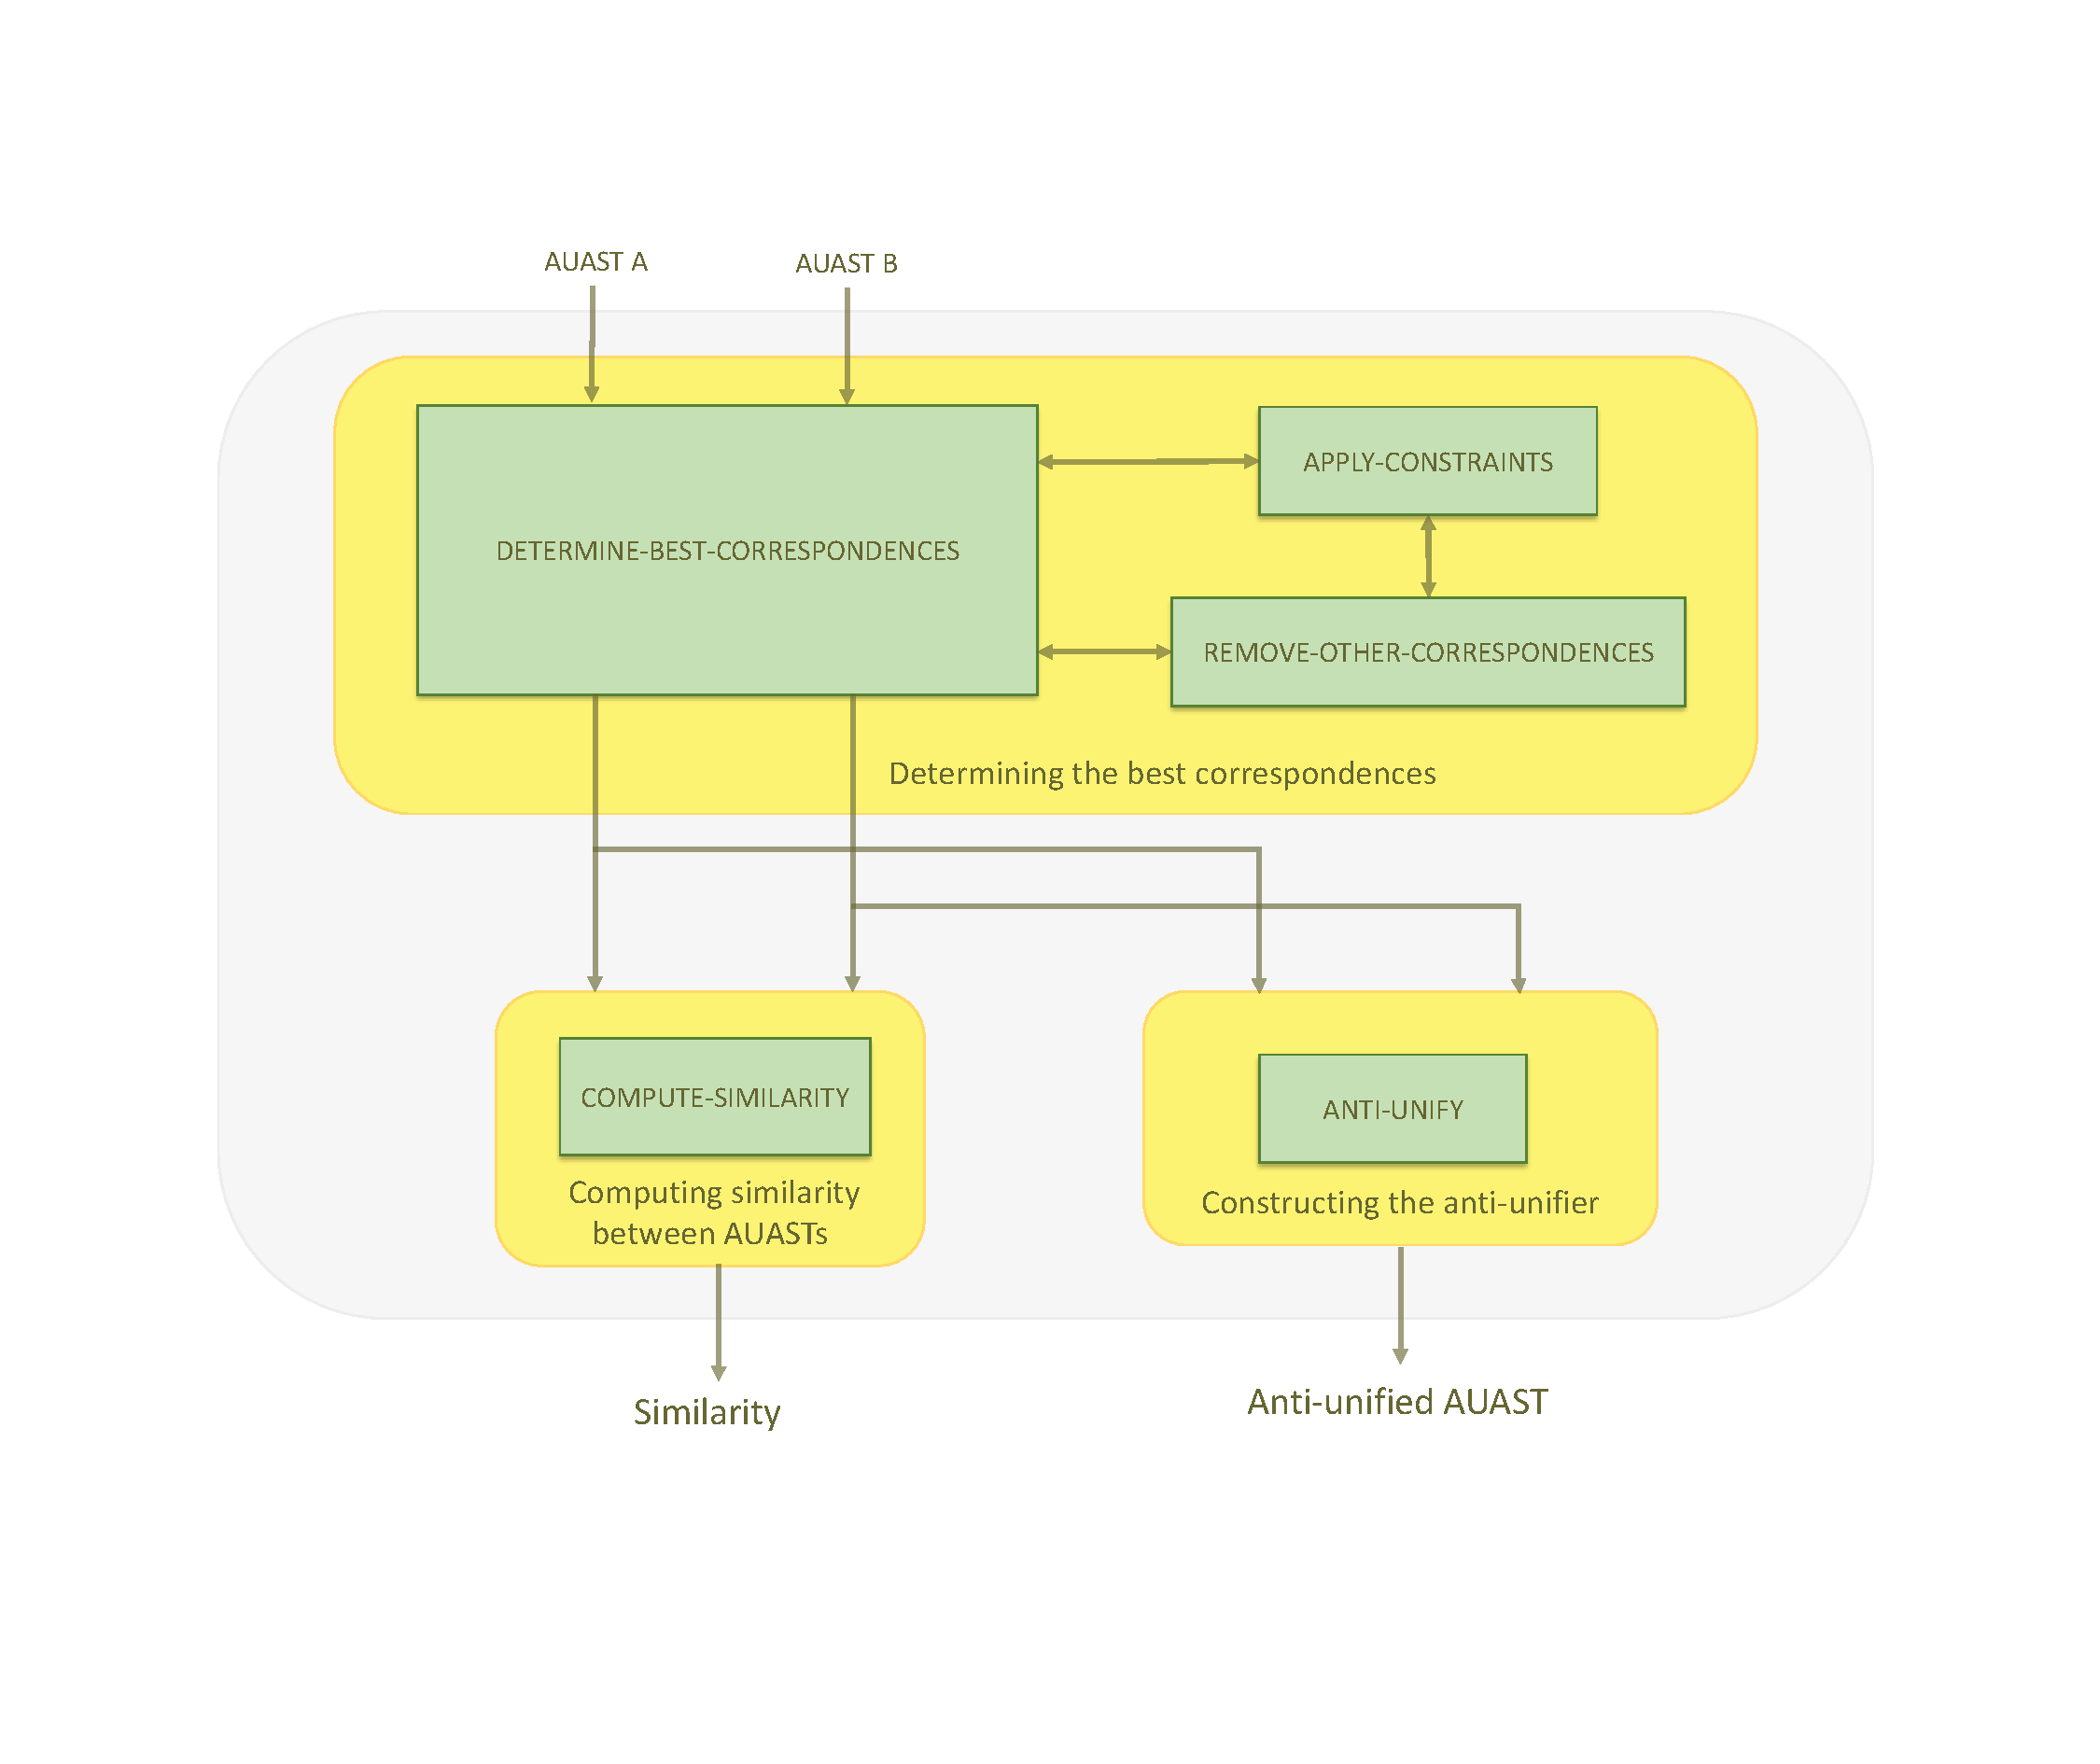
\includegraphics [width = \textwidth]{Drawing4/auOverview.pdf}
  \caption{Overview of the anti-unification process.}
  \label{fig:meth_overview}
\end{figure}


To evaluate my approach, I developed the anti-unifier-building tool atop Jigsaw, and conducted an experimental study on the test suite introduced in Section~\ref{study1_setup}. In Section~\ref{antiunifierTool}, I discuss the algorithms and decisions I made for implementing the anti-unifier-building tool and constructing a detailed view of the structural generalization. I also describe my experimental setup, present the study, and discuss the results in Section~\ref{anti-unifier-assessment}.



%abstracts structural correspondences of ASTs
%A generalization mechanism could be used to abstract commonalities in several structures containing logging calls into a more general structure;
%The higher-order anti-unification modulo theories framework could assist us in constructing a structural generalization from a pair of LCSs. Also, A modified version of a hierarchical clustering suited for our application could assist us to construct a generalization from a set of LMs.

%To construct a structural generalization from a pair of LMs, we developed a prototype tool that applies the Jigsaw framework to find candidate correspondences between two ASTs and uses higher-order anti-unification modulo theories to generalize the structures. It takes the source code of two logged \name{Java} methods as input and performs a sequence of six actions on them, outlined by the algorithm \func{Anti-unification}: (1) we input into the algorithm the ASTs of two given logged \name{Java} methods, constructed via the Eclipse Java Development Tools (JDT) framework; (2) we generate an augmented form of AST (called a CAST) using the Jigsaw framework, where each node holds a list of candidate correspondence connections between the two ASTs (line~1) (see Section~\ref{meth-CAST}); (3) we extend the CAST structure to a higher-order extended structure (called an AUAST) and apply some constraints to prevent the anti-unification of logging calls with anything else (lines~2--3) (see Sections~\ref{meth-constructAUAST} and~\ref{meth-constraints}); (4) we determine the best correspondence for each node of the AUASTs with the highest similarity and we remove the other correspondence connections involving the nodes (line~4) (see Section~\ref{meth-correspondence}); (5) we anti-unify structural properties with their best correspondence to construct an approximation of the best anti-unifier to our problem with special attention to logging calls (line~5) (see Section~\ref{meth-antiUnifier}); and (6) we measure similarity (line~6) (see Section~\ref{meth-similarity}).
%\begin{algorithm}
%\caption{Input into \func{Anti-unification}(\id{auastA},\id{auastB}) are AUAST nodes of two \name{Java} classes containing logging calls; this algorithm construct an anti-unified AUAST node through anti-unification of input node's structural properties} %and compute similarity between them with a focus on logging calls}
%\label{overview}
%\begin{algorithmic}[1]
%\antiunification
%    \State  $\func{Jigsaw-Correspondence}(\id{auastA},\id{auastB})$
%   \State $\id{auastA}, \id{auastB} \gets \func{Apply-Constrains}(\id{auastA},\id{auastB})$
%   \State $$list}  \gets \func{Determine-Best-Correspondences}(\id{auastA})$
%     \State $$compute-similarity} \gets \func{Compute-Similarity}(\id{auastA},\id{auastB})$
%    \State $$anti-unifier} \gets \func{Antiunify}(\id{auastA},\id{auastB})$
%\end{algorithmic}
%\end{algorithm}


%\section{Anti-unification of a pair of ASTs} \label{anti-unification pairs}
%\subsection{Anti-unification ASTs}\label{AUAST}
%\RW{Describe testing/evaluation.}


%\section{Anti-unification ASTs} \label{anti-unification pairs}






\section{Determining the best correspondences}  \label{best-corr}
%As described in Section~\ref{Jigsaw}, through the application of Jigsaw, each AUAST node will hold a list of candidate correspondence connections, each implicitly representing an anti-unifier. However, despite having multiple potential anti-unifiers, we need to determine one single anti-unifier that is helpful to solve our problem using the greedy selection algorithm discussed in Section~\ref{}.


As discussed in Section~\ref{HOAUMT}, the complexity of determining the best anti-unifier is undecidable in general. Therefore, to find one single anti-unifier that is an approximation of the optimal fit to my problem, I developed the \func{Determine-Best-Correspondences} algorithm that greedily selects the most similar correspondence as the best fit for each AUAST node. Therefore, each AUAST node can either be anti-unified with its best correspondence in the other AUAST or with \nothing. This algorithm takes one of the AUASTs, visiting the AUAST nodes therein to store all candidate correspondence connections between the two AUAST nodes in a list, which is sorted in descending order based on the similarity measure (lines~1--9). However, to prevent the anti-unification of log statement nodes with any other nodes, some constraints should be applied on the selection of correspondence connections prior to determining the best ones via the \func{Apply-Constraints} algorithm (Line~8). Then the correspondence connection with the highest similarity value is determined as the best fit for the two nodes involved, and all other correspondence connections involving these nodes are removed using \func{Remove-Other-Correspondences} algorithm (lines~10--14). This process terminates when no more correspondence connections are left in the list.

%entire --> one single

\begin{algorithm}
\caption{\func{Determine-Best-Correspondences}($\id{a}$) takes in the one of the AUASTs and determines the best correspondence connection with the highest similarity for each node.}
\label{alg-determine}
\begin{algorithmic}[1]
\DetermineBest
    \State $\id{list} \gets \func{()}$
    \State $\id{nodes} \gets \func{visitor}(\id{a})$
	  \For {$\id{nodeA} \in \id{a}$}
		\For {$\id{corr} \in  \id{corrs}[\id{nodeA}]$}		
				 	\State{$\func{Append}(\id{corr},\id{list})$ }
			 	\EndFor  	
	   \EndFor	
	    \State{$ \func{Apply-Constraints}(\id{list}) $}	
	   \State{$\func{sort}(\id{list})$}
	   \For{$\id{corr} \in \id{list}$}
	   		\State $\id{bestCorr}[\id{nodeA}] \gets \id{corr}$
	   		\State $\id{bestCorr}[\id{nodeB}] \gets \id{corr}$
	   		\State{$\func{Remove-Other-Correspondences}(\id{corr},\id{list})$ }
	   \EndFor
 %\Return $\id{list} $  	
  \end{algorithmic}
\end{algorithm}

To construct an anti-unifier of the AUASTs of logged methods with a focus on logging calls, some constraints should be applied in determining correspondences. The first constraint (as described below) should be applied to prevent the anti-unification of log statement nodes with any other types of nodes.
\begin{constraint}
A logging call should either be anti-unified with another logging call or should be anti-unified with \nothing.
\end{constraint}	
	
This constraint creates a further constraint:

\begin{constraint}
A structure containing a logging call should be anti-unified with a corresponding structure containing another logging call or should be anti-unified with \nothing.
\end{constraint}

As an illustration consider the CASTs of the two examples in Figure~\ref{fig:meth-ast-1}. As it is shown, there is a candidate correspondence connection between the two log method invocation nodes and the two \code{if} statements. As is clear, the second \code{if} statement contains a logging call, while there is no corresponding logging call in the first one. According to the first constraint, two log method invocation nodes should be anti-unified together. On the other hand, a correspondence connection is created between the two \code{if} statements; however, anti-unification of these statements includes anti-unifying their children nodes as well. Thus, statements inside the body of the \code{if} statements must be anti-unified with each other, indicating that log method invocation inside the body of \code{if} statement in the second example should be anti-unified with \nothing, which is contrary to our first assumption. In order to comply with the first constraint, the correspondence connection between two \code{if} statements should be deleted, leading us to apply the second constraint. My approach applies these constraints by taking the following steps prior to determining the best correspondences:
\begin{enumerate} [leftmargin=.4in]
\item	Augment a property to the AUAST node to mark log statement nodes and structures enclosing them as ``logged''.
\item	Remove correspondence connections where one node is marked as ``logged'' and the corresponding node is not via the \func{Apply-Constraints} algorithm.
\end{enumerate}

The \func{Apply-Constraints} algorithm takes the list of correspondence connections, and removes the ones involving two nodes where one is ``logged'' and the corresponding node is not, using the \func{Remove-Other-Correspondences} algorithm (lines~1--9).

\begin{algorithm}
  \caption{\func{Apply-Constraints}($\id{list}$) applies the constraints on the list of correspondence connections.}
  \label{computeMatches}
  \begin{algorithmic}[1]
  \ApplyConstraints
      \For {$\id{corr} \in \id{list}$}
      \State $\id{nodeA} \gets \id{nodeA}[\id{corr}]$
	  \State $\id{nodeB} \gets \id{nodeB}[\id{corr}]$
 			\If {($\id{nodeA} \Instanceof \cons{Logged}) \And (\id{nodeB} \Instanceof \cons{Non-Logged}$)}	
 		\State{$\func{Remove-Other-Correspondences}(\id{corr},\id{list})$ }
	   	\ElsIf {$(\id{nodeA} \Instanceof \cons{Non-Logged}) \And (\id{nodeB} \Instanceof \cons{Logged}$) }	
  		\State{$\func{Remove-Other-Correspondences}(\id{corr},\id{list})$ }
	  \EndIf 		
 \EndFor 	
	
  \end{algorithmic}
\end{algorithm}




\func{Remove-Other-Correspondences} algorithm removes correspondence connections that are not selected as the best fit from three lists: the list of all correspondence connections (Line~5 and Line~12);
the list of correspondence connections of the first node involved in the connection (Line~6 and Line~13); the list of correspondence connections of the second node involved in the connection (Line~7 and Line~14). As an example, Figure~\ref{fig:AUASTs} shows the correspondence connections between AUAST nodes after applying the \func{Determine-Best-Correspondence} algorithm on the list of potential correspondence connections.
%in Figure~\ref{fig:meth-ast-1}.

\begin{algorithm}
\caption{\func{Remove-Other-Correspondences}($\id{corr}$,$\id{list}$) removes all other correspondences involving the nodes of a particular correspondence connection ($\id{corr}$) from the lists of correspondences.}
\label{removeOtherCEs}
  \begin{algorithmic}[1]
  \RemoveOtherCEs
       \State $\id{listA} \gets \id{corrs}[\id{nodeA}[\id{corr}]]$
	   \State $\id{listB} \gets \id{corrs}[\id{nodeB}[\id{corr}]]$
	   \For {$\id{corrA} \in \id{listA}$}
			\If{$\id{corrA} \neq \id{corr}$}	
\State{$\func{Remove}(\id{corrA},\id{listA})$ } 			
\State{$\func{Remove}(\id{corrA},\id{corrs}[\id{nodeA}[\id{corrA}]])$ }
\State{$\func{Remove}(\id{corrA},\id{corrs}[\id{nodeB}[\id{corrA}]])$ }    		
	   		 \EndIf
	   \EndFor		
       \For {$\id{corrB} \in \id{listB}$}
			\If{$\id{corrB} \neq \id{corr}$}	   		 	 	
	 	 	\State{$\func{Remove}(\id{corrB},\id{listB})$ } 		 \State{$\func{Remove}(\id{corrB},\id{corrs}[\id{nodeA}[\id{corrB}]])$ }
\State{$\func{Remove}(\id{corrB},\id{corrs}[\id{nodeB}[\id{corrB}]])$ }
	   		 \EndIf
	   \EndFor	  	
  \end{algorithmic}
\end{algorithm}




\begin{figure} [H]
  \centering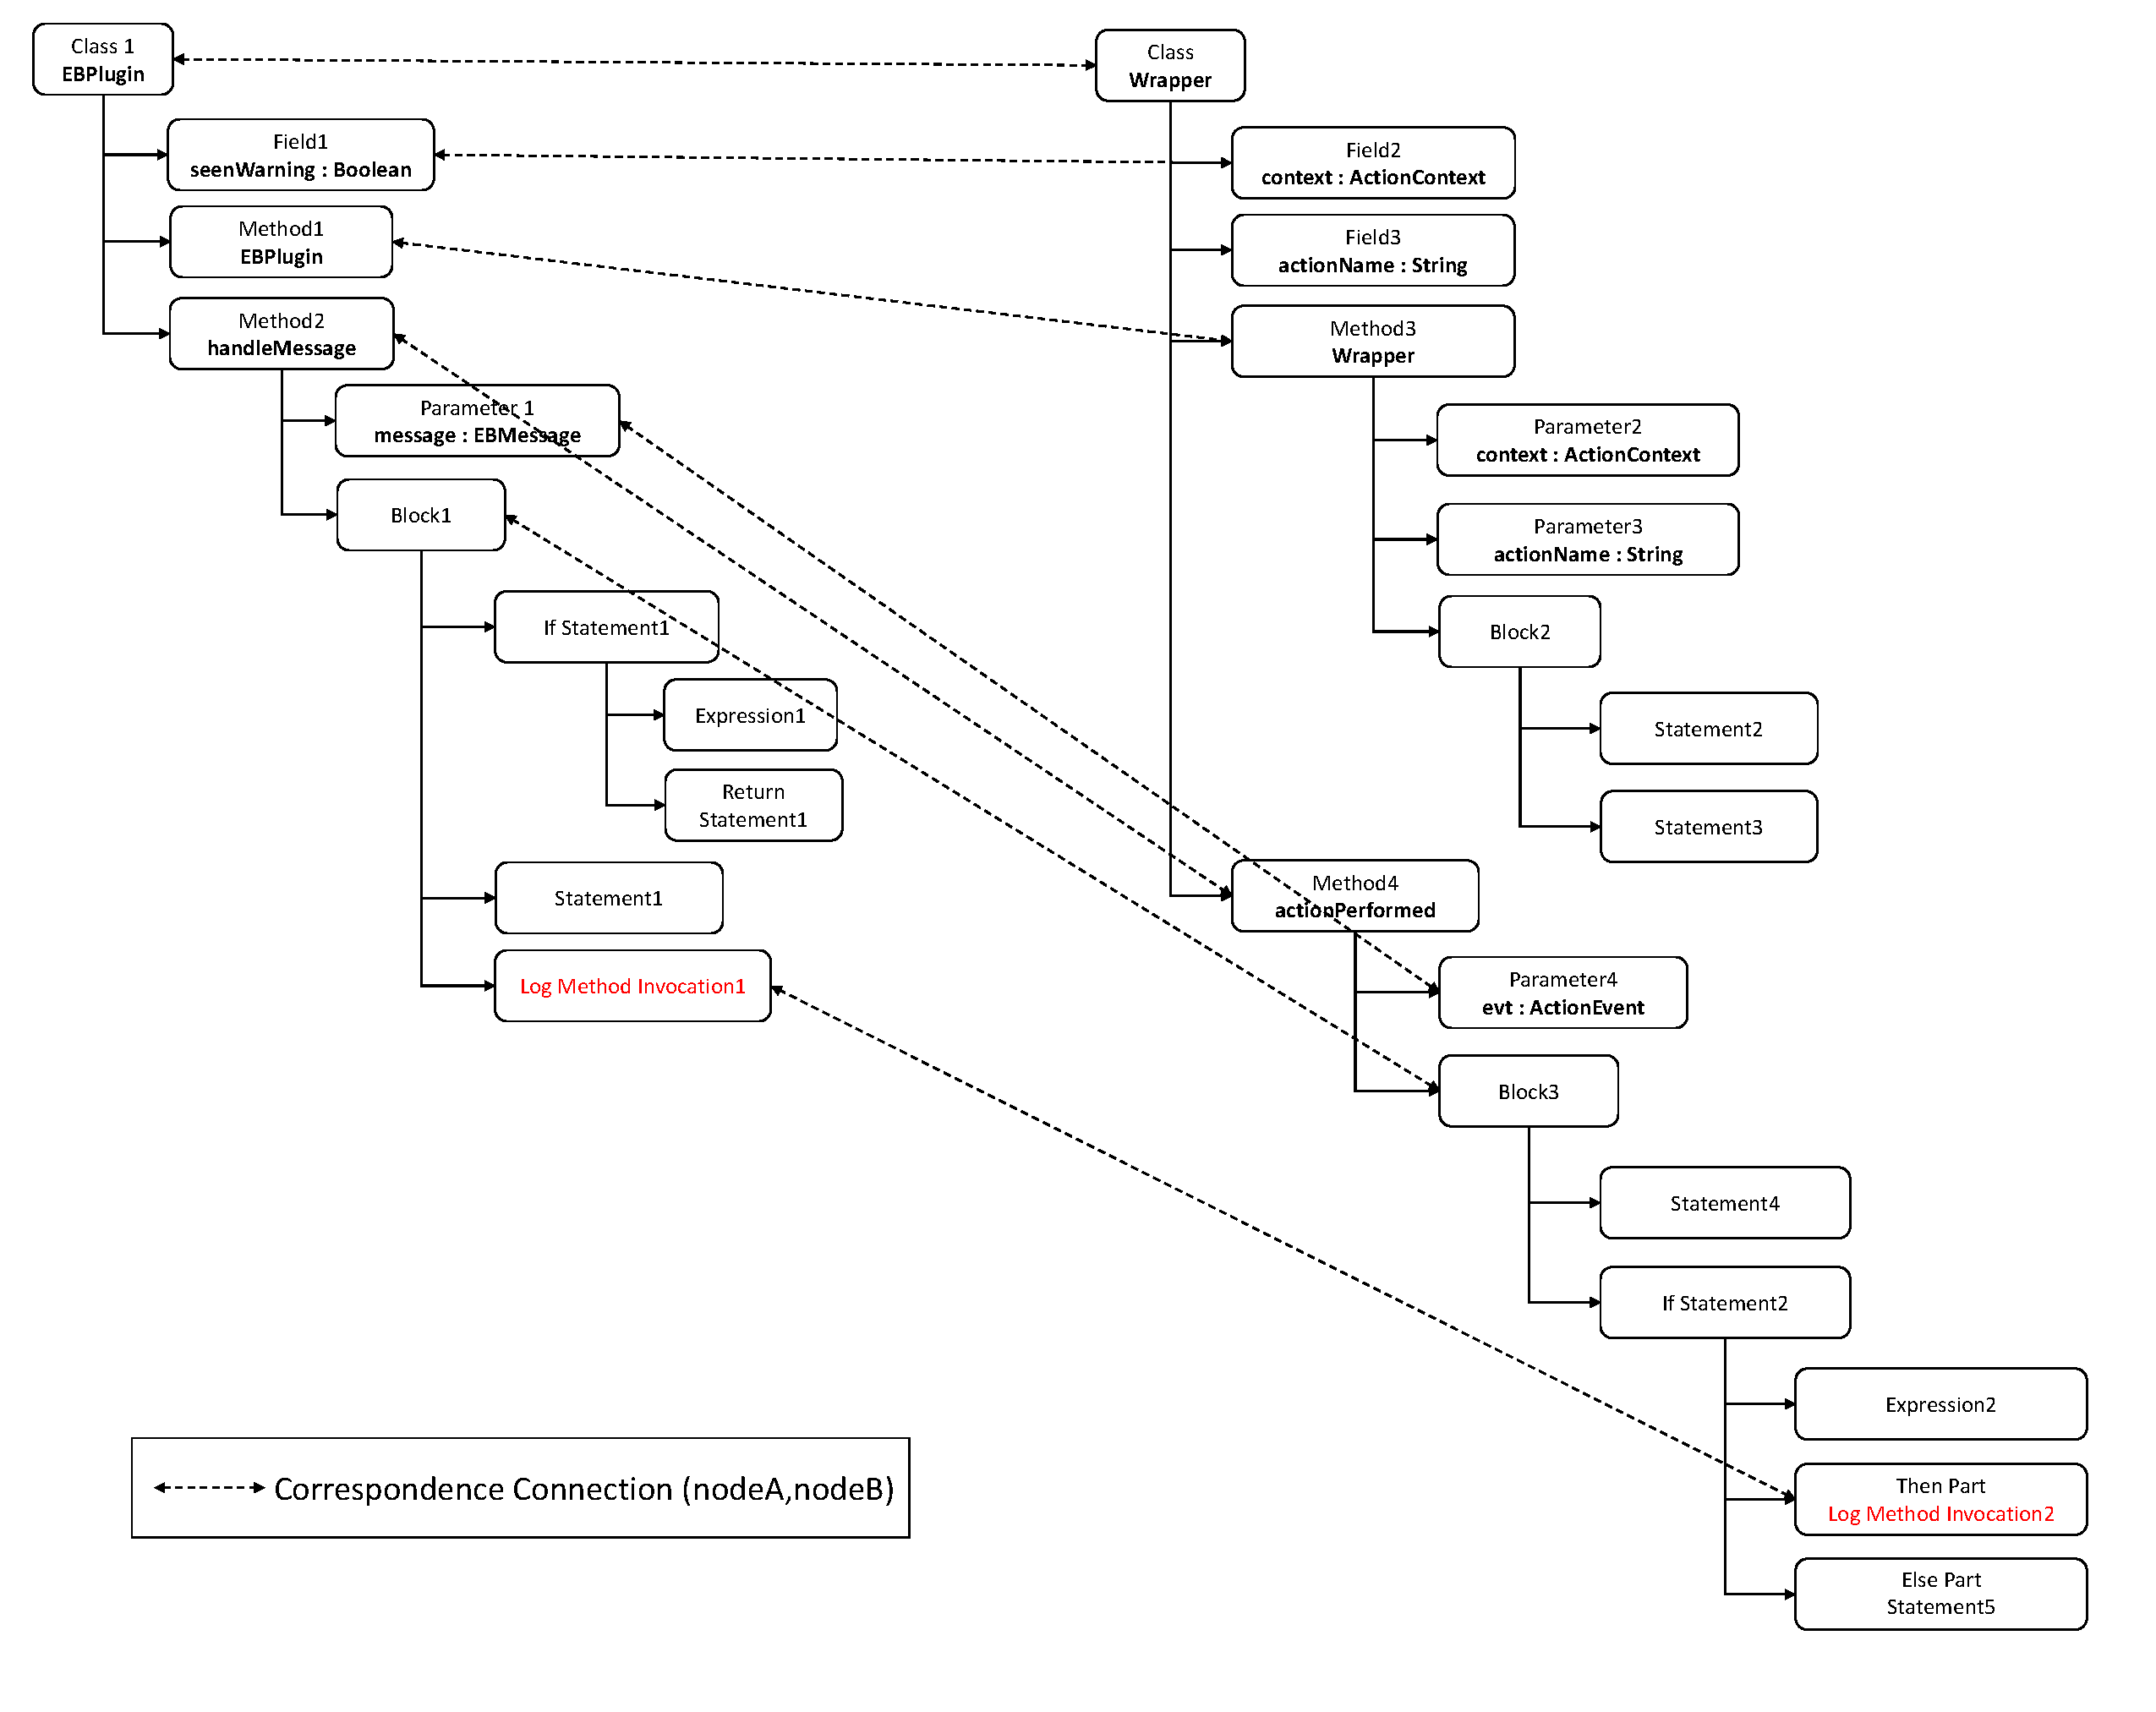
\includegraphics [width = \textwidth]{Drawing4/FinalCorr.pdf}
  \caption{Simple AUAST structure of examples in Figures~\ref{ch3-ex1} and~\ref{ch3-ex2}. The links between AUAST nodes indicate structural correspondences selected as the best fit using the \func{Determine-Best-Correspondences} algorithm.}
  \label{fig:AUASTs}
\end{figure}
%In general, higher order anti-unification modulo theories is undecidable [Cottrell et al., 2008]. That is, the complexity of determining the most optimal MSA is undecidable, but our desire is to create one of the best MSAs to approximate the optimal one that can sufficiently solve our problem, thus the anti-unification process should construct an anti-unifier that is the best approximate fit for our application. To this end, a greedy selection algorithm has been used, which is an approximation technique to determine the best correspondence for each node in the AUAST so constructing the anti-unifier that is approximately the best fit to our problem.

\section{Computing similarity between AUASTs} \label{meth-similarity}
Similarity computation is particularly important for clustering phase that relies on accurate estimation of similarity between logged methods (Chapter~\ref{clustering}). The notion of similarity can differ depending on the given context. That is, similarity between certain features could be highly important for a particular application, while it is not for another. The utility of a similarity function can be determined based on how well it enables us to produce accurate results for a particular task. In this study, a similarity measure is needed to classify logged methods based on the structural similarity in the usage of logging calls. The similarity for my application can be defined as the number of common elements over the total number of elements of the anti-unifier constructed based on the selected correspondences from the previous step.

%computed the ratio of the number of common elements over the total number of elements of the anti-unifier to measure similarity between two AUASTs


% Equation???
% heuristic???

The similarity between two AUAST nodes is computed by dividing the number of matched elements among the two nodes by the size of the largest node (Equation~\ref{eq-jigsaw-sim}). The number of matches between the two AUASTS $\id{a}$ and $\id{b}$ is computed via the \func{Compute-Best-Matches} algorithm. If the two AUASTs are of leaf nodes, the number of matches is computed using the heuristics proposed by \citet{2008:fse:cottrell} (Section~\ref{Jigsaw}) (Lines~2--3). Otherwise, the best correspondences between the two subtrees are selected using the \func{Determine-Best-Correspondences} algorithm, and the matches between each children of the subtree $\id{a}$ and its best corresponding node in the subtree $\id{b}$ is computed and propagated to the parent node (Lines~4--12).


\begin{algorithm}
 \caption{\func{Compute-Best-Matches}($\id{a}$,$\id{b}$) computes the matches between the two ASTs based on the best correspondences.}
  \label{simi}
  \begin{algorithmic}[1]
  \ComputeBestMatches
  \State $\id{matches} \gets 0$
\If {$\id{a} \Instanceof \cons{Leaf-Node}$ }	
  \State $\id{matches} \gets   \func{matches}(\id{a},\id{b})$
  \ElsIf {$\id{a} \Instanceof \cons{Non-Leaf-Node}$ }	
    	\State \func{Determine-Best-Correspondences}($\id{a}$, $\id{b}$)
\For {$\id{childA} \in \id{children}[\id{a}]$}
\If {$ \id{bestCorr}[\id{childA}] \neq \cons{NULL}$}	 		
	%\State $\id{childB}\gets \id{bestCorr}[\id{childA}]$ 		
 		\State $\id{matches} \gets \id{matches}+\func{Compute-Best-Matches}(\id{childA},\id{node}[\id{bestCorr}[\id{childA}]])$		 
 \EndIf
 \EndFor

 \EndIf
 \Return $matches$
\end{algorithmic}
\end{algorithm}



%NIL->0????


%The number of identical structural properties between $\id{auastA}$ and $\id{auastB}$ is computed via the \textsc{Compute-Matches} algorithm through a recursive traversal of $\id{antiunifier}$ nodes' structural properties. For simple structural properties, the number of matches is added by one (Lines~3-4). For child structural properties, the number of matches is added by one and the number of matches computed recursively for the child node (Lines~5-8). For child list structural properties, the number of matches is computed for each child node recursively and is propagated to the parent node (Lines~9-13). All matches are summed up to compute total number of matches between the two AUASTs. Then the following equation is used to compute structural similarity between $\id{auastA}$ and $\id{auastB}$:

\section{Constructing the anti-unifier} \label{meth-antiUnifier}
Once the best correspondences have been determined between two AUASTs, I construct a new anti-unified AUAST by traversing the original AUAST structures recursively and anti-unifying each node with its best correspondence. The new anti-unified structure is a generalization of two original structures, called anti-unifier, where common structural properties are represented by copies and differences are represented by structural variables. The variables may be inserted in place of any node in AUAST, including both subtrees and leaves, and can be substituted with proper original substructures to regain original structures.


% anti-unify the same type nodes????????

Anti-unification of two AUASTs is performed via the \func{Antiunify} algorithm. If the two AUASTs are of leaf nodes, the anti-unifier will be created through the anti-unification of the two nodes (Lines~2--3). Otherwise, the anti-unified subtree is created by anti-unifying each children of one subtree with its best corresponding node in the other subtree. If there is no correspondence for a node, the anti-unified node will be created through the anti-unification of the node with the \NIL{} structure. All these anti-unified nodes are appended to the list of children of the anti-unifier (Lines~4--21). The details of constructing a detailed view of the anti-unifier for my application will be discussed in Section~\ref{meth-detailed-view}.


\begin{algorithm}
 \caption{\func{Antiunify}($\id{a}$,$\id{b}$) creates the anti-unifier of two AUASTs through the anti-unification of each node with its best correspondence.}
  \label{AntiUnify}
  \begin{algorithmic}[1]
\AntiUnify
\State{$ \id{antiunifier} \gets \cons{Null}$}
\If {$\id{a} \Instanceof \cons{Leaf-Node}$ }	
  \State $\id{antiunifier} \gets   \func{construct-antiunifier}(\id{a},\id{b})$
  \ElsIf {$\id{a} \Instanceof \cons{Non-Leaf-Node}$ }	
 % \State \func{Determine-Best-Correspondences}($\id{a}$, $\id{b}$)
        \For {$\id{childA} \in \id{children}[\id{a}]$}
\If {$ bestCorr[childA]= \cons{NULL}$}	
  \State $\id{child} \gets   \func{Antiunify}(\id{childA},\cons{NIL})$
\Else	
 \State $\id{child} \gets   \func{Antiunify}(\id{childA},\id{node}[bestCorr[childA]])$
\EndIf
\State $\func{Append}(\id{child},\id{children[antiunifier]})$
\EndFor
%	\EndIf	
  %\If {$\id{b} \Instanceof \cons{Non-Leaf-Node}$ }	
\EndIf
  \If {$\id{b} \Instanceof \cons{Non-Leaf-Node}$ }	

  \For {$\id{childB} \in \id{children}[\id{b}]$}
\If {$ bestCorr[childB]= \cons{NULL}$}	
  \State $\id{child} \gets   \func{Antiunify}(\id{childB},\cons{NIL})$
\EndIf
\State $\func{Append}(\id{child},\id{children[antiunifier]})$
\EndFor
 \EndIf
\Return $\id{antiunifier}$
\end{algorithmic}
\end{algorithm}



\section{The Anti-unifier building tool} \label{antiunifierTool}
The anti-unifier building tool is a proof-of-concept implementation of my anti-unification approach, which is developed atop the Jigsaw framework to construct a detailed view of structural generalization. To create the AUAST structure using Eclipse JDT framework that addresses the limitations of CAST to constructing an anti-unifier, I added the following structural properties:
%namely?
%to address the limitations of CAST to constructing an anti-unifier
%It also creates an extended form of CAST, called AUAST,
\begin{itemize} [leftmargin=.5in]
\item \textit{Simple structural variable Properties}: an extension of simple structural properties referring to two simple values to allow the insertion of variables in place of leaves.
\end{itemize}
\begin{itemize} [leftmargin=.5in]
\item \textit{Child structural variable properties}: an extension of child structural properties referring to two child AST nodes to allow the insertion of variables in place of subtrees.
\end{itemize}

I also needed to make additional algorithms and decisions to construct a detailed generalization view suited to my application, which will be described in the following sections.

%%change???


\subsection{Constructing the detailed generalization view} \label{meth-detailed-view}

To figure out the structural commonalities and differences amongst logged methods, I developed an algorithm to construct a generalization view of the anti-unifier. Figure~\ref{fig:meth-anti-unifier} shows a simple detailed view I used to represent the anti-unifier constructed from the AUASTs of logged methods of Examples 1 and 2, where ``$\id{a}$-or-$\id{b}$'' represents a structural variable that must be substituted with either the $a$ or $b$ substructures to recover each original structure, and ``$\id{a}$'' represents that the $a$ substructure is common between the two AUASTs.
%??????


% modify the figure???

\begin{figure} [H]
  \centering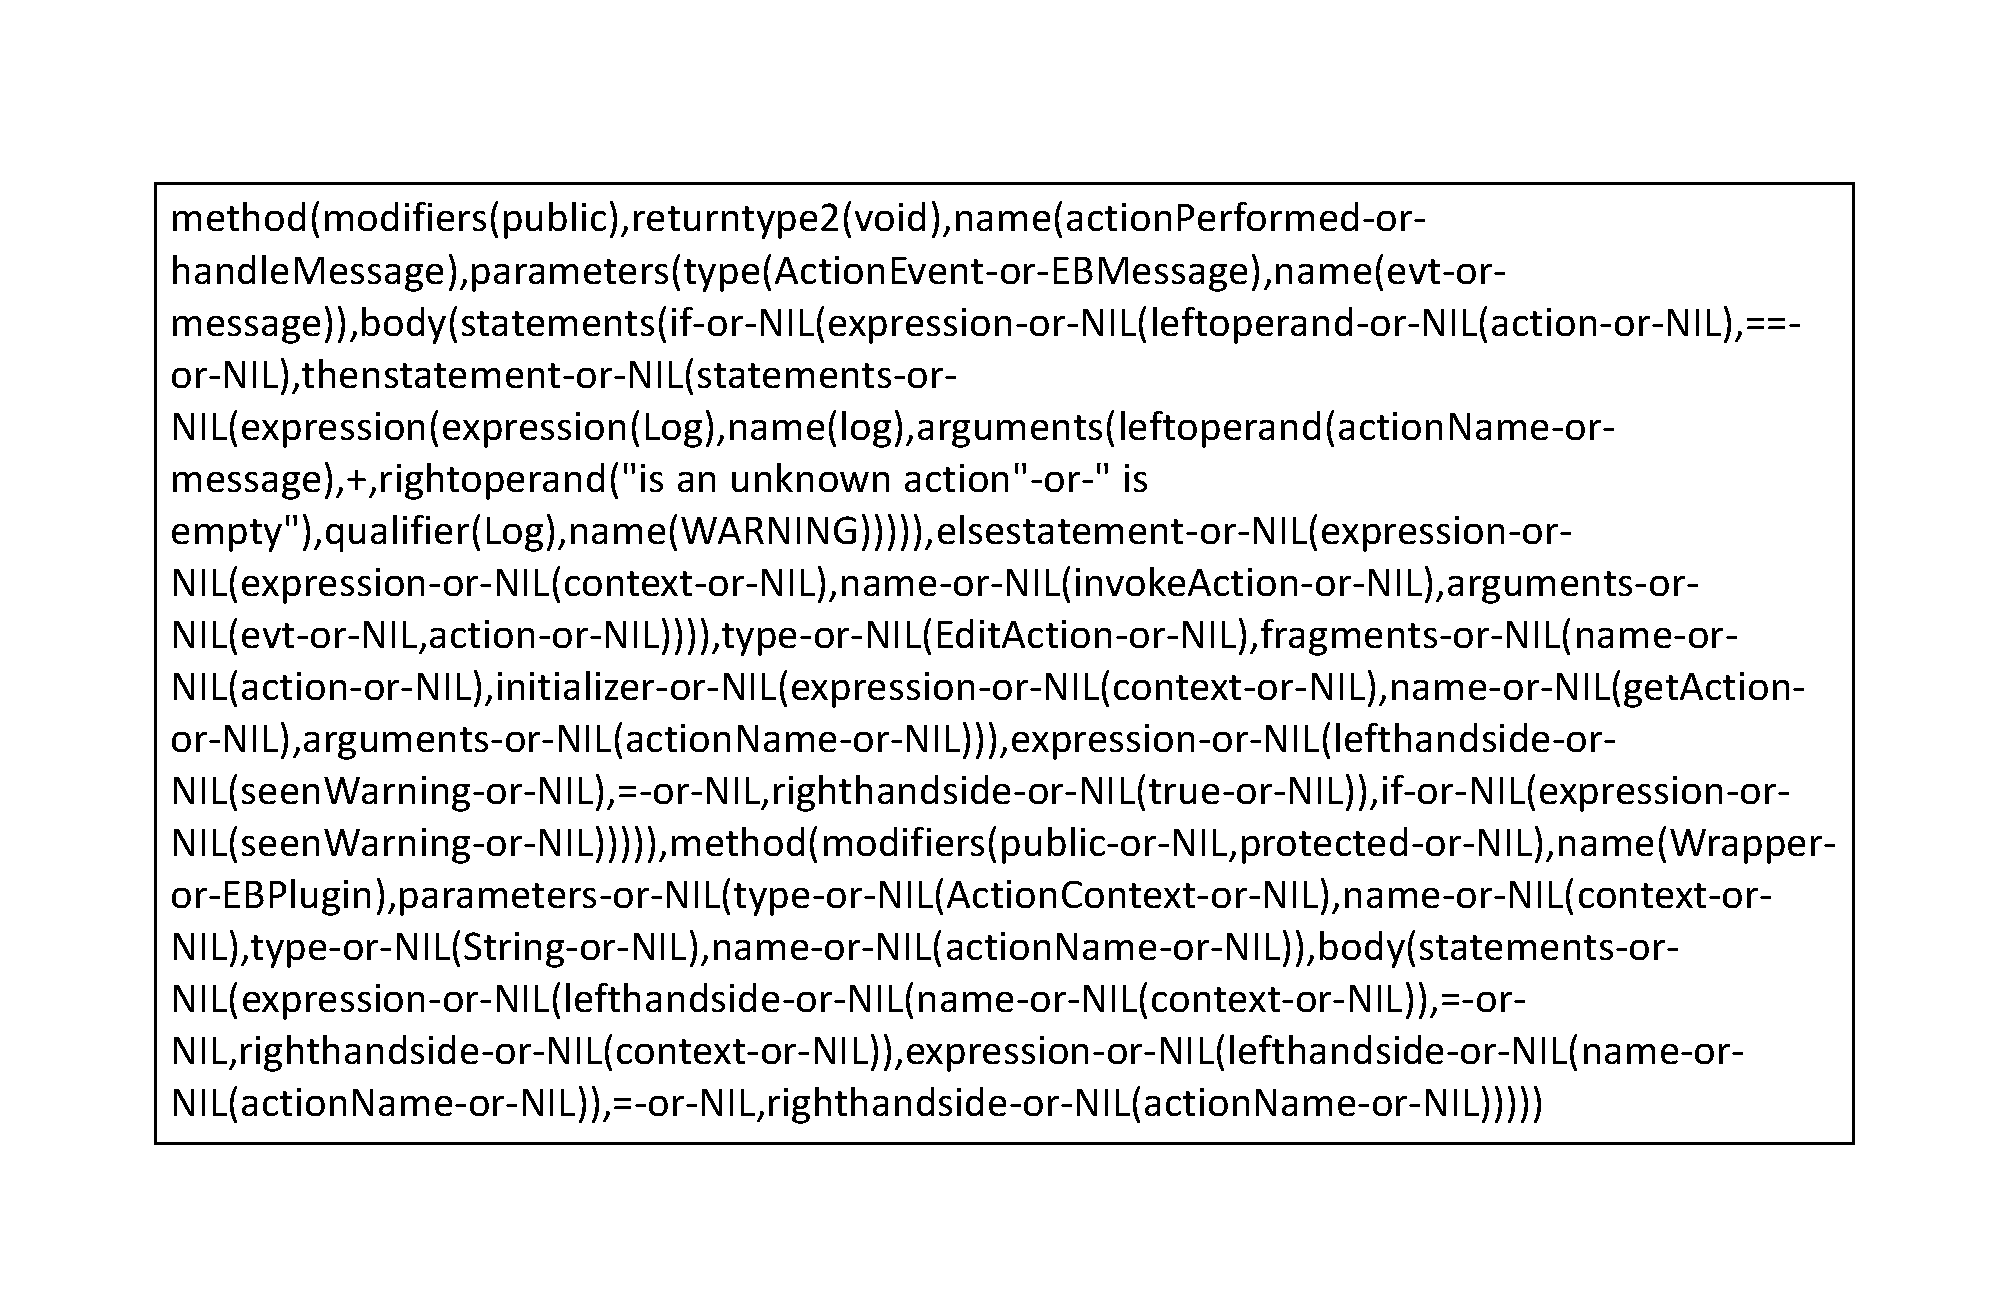
\includegraphics [scale=0.5]{Drawing4/auMethod.pdf}
  \caption{Simple detailed view of the anti-unifier constructed from the AUASTs of Examples 1 and 2.}
  \label{fig:meth-anti-unifier}
\end{figure}

% the LMs in
% to create an anti-unifier description. For example, we supply the \func{Antiunify} algorithm with the AUASTs of LMs in Examples 1 and 2
%explain in more details???

To create the detailed view of the structural generalization from two given AUASTs, I applied the \func{Antiunify} algorithm presented in Section~\ref{meth-antiUnifier} on the two AUAST nodes $\id{a}$ and $\id{b}$ through the anti-unification of their structural properties, as the Eclipse JDT utilizes these properties to record structural information of each \name{Java} element (Section~ref{JDT}). That is, for each structural property of the two nodes, if the property is common between them, a copy of it will be created and added to the structural properties of the anti-unifier; otherwise, a variable structural property is constructed referring to two property values and and added to the anti-unifier's structural properties.
%property values???


% (Lines~8--9); if structural property is a child property, a child variable structure is constructed (Lines~10--12). All these strcutural prperties will be added to the structural property of the anti-unifier(Lines~8--9). 


%if structural property is a child list property, for each child of $\id{propA}$ and $\id{propB}$, where there is no correspondence in the other AUAST, an anti-unified node is created through the anti-unification of the child node with the \NIL{} structure via the \func{Antiunify} algorithm and added to the value of the anti-unified child list property; otherwise, the child node is anti-unified with its best correspondence (Lines~6-21).


\subsection{Java methods containing multiple logging calls} \label{meth-multipleLogs}
There might be some cases in which our approach is not able to anti-unify logging calls in two input seeds, when there is more than one logging call in a LJM. For example, consider the LMs in Figures~\ref{multiple1} and~\ref{multiple2}. Figure~\ref{mast_1} shows the simple AUASTs for these examples and potential correspondence connections between the AUAST nodes. Figure~\ref{m_ast2} shows the correspondence connections selected as the best match using our greedy algorithm. To anti-unify \code{if statement 1} with \code{if statement 3}, we should anti-unify their structural properties. Thus, \code{log1} should be anti-unified with \code{log3}, and \code{log4} should be anti-unified with \NIL{} since there is no corresponding logging call in the body of \code{if statement 1}, while there is a corresponding logging call for \code{log4} in the body of \code{if statement 2} (\code{log2}).

%\code{if statement 1}???
%In figures: If statement: if statement 1???

\begin{figure}[H]
\def\baselinestretch{1}
\begin{lstlisting}
public void method1(){
	...
	if(condition1){
		Log.log();
	}
	...
	if(condition2){
		Log.log();
	}
	...
}
\end{lstlisting}
\caption{A \name{Java} method that utilizes multiple logging calls.\label{multiple1}}
\end{figure}



\begin{figure}[H]
\def\baselinestretch{1}
\begin{lstlisting}
public void method2(){
	...
	if(condition3){
		Log.log();
		Log.log();
	}
	...
}
\end{lstlisting}
\caption{A \name{Java} method that utilizes multiple logging calls.\label{multiple2}}
\end{figure}

\begin{figure} [H]
  \centering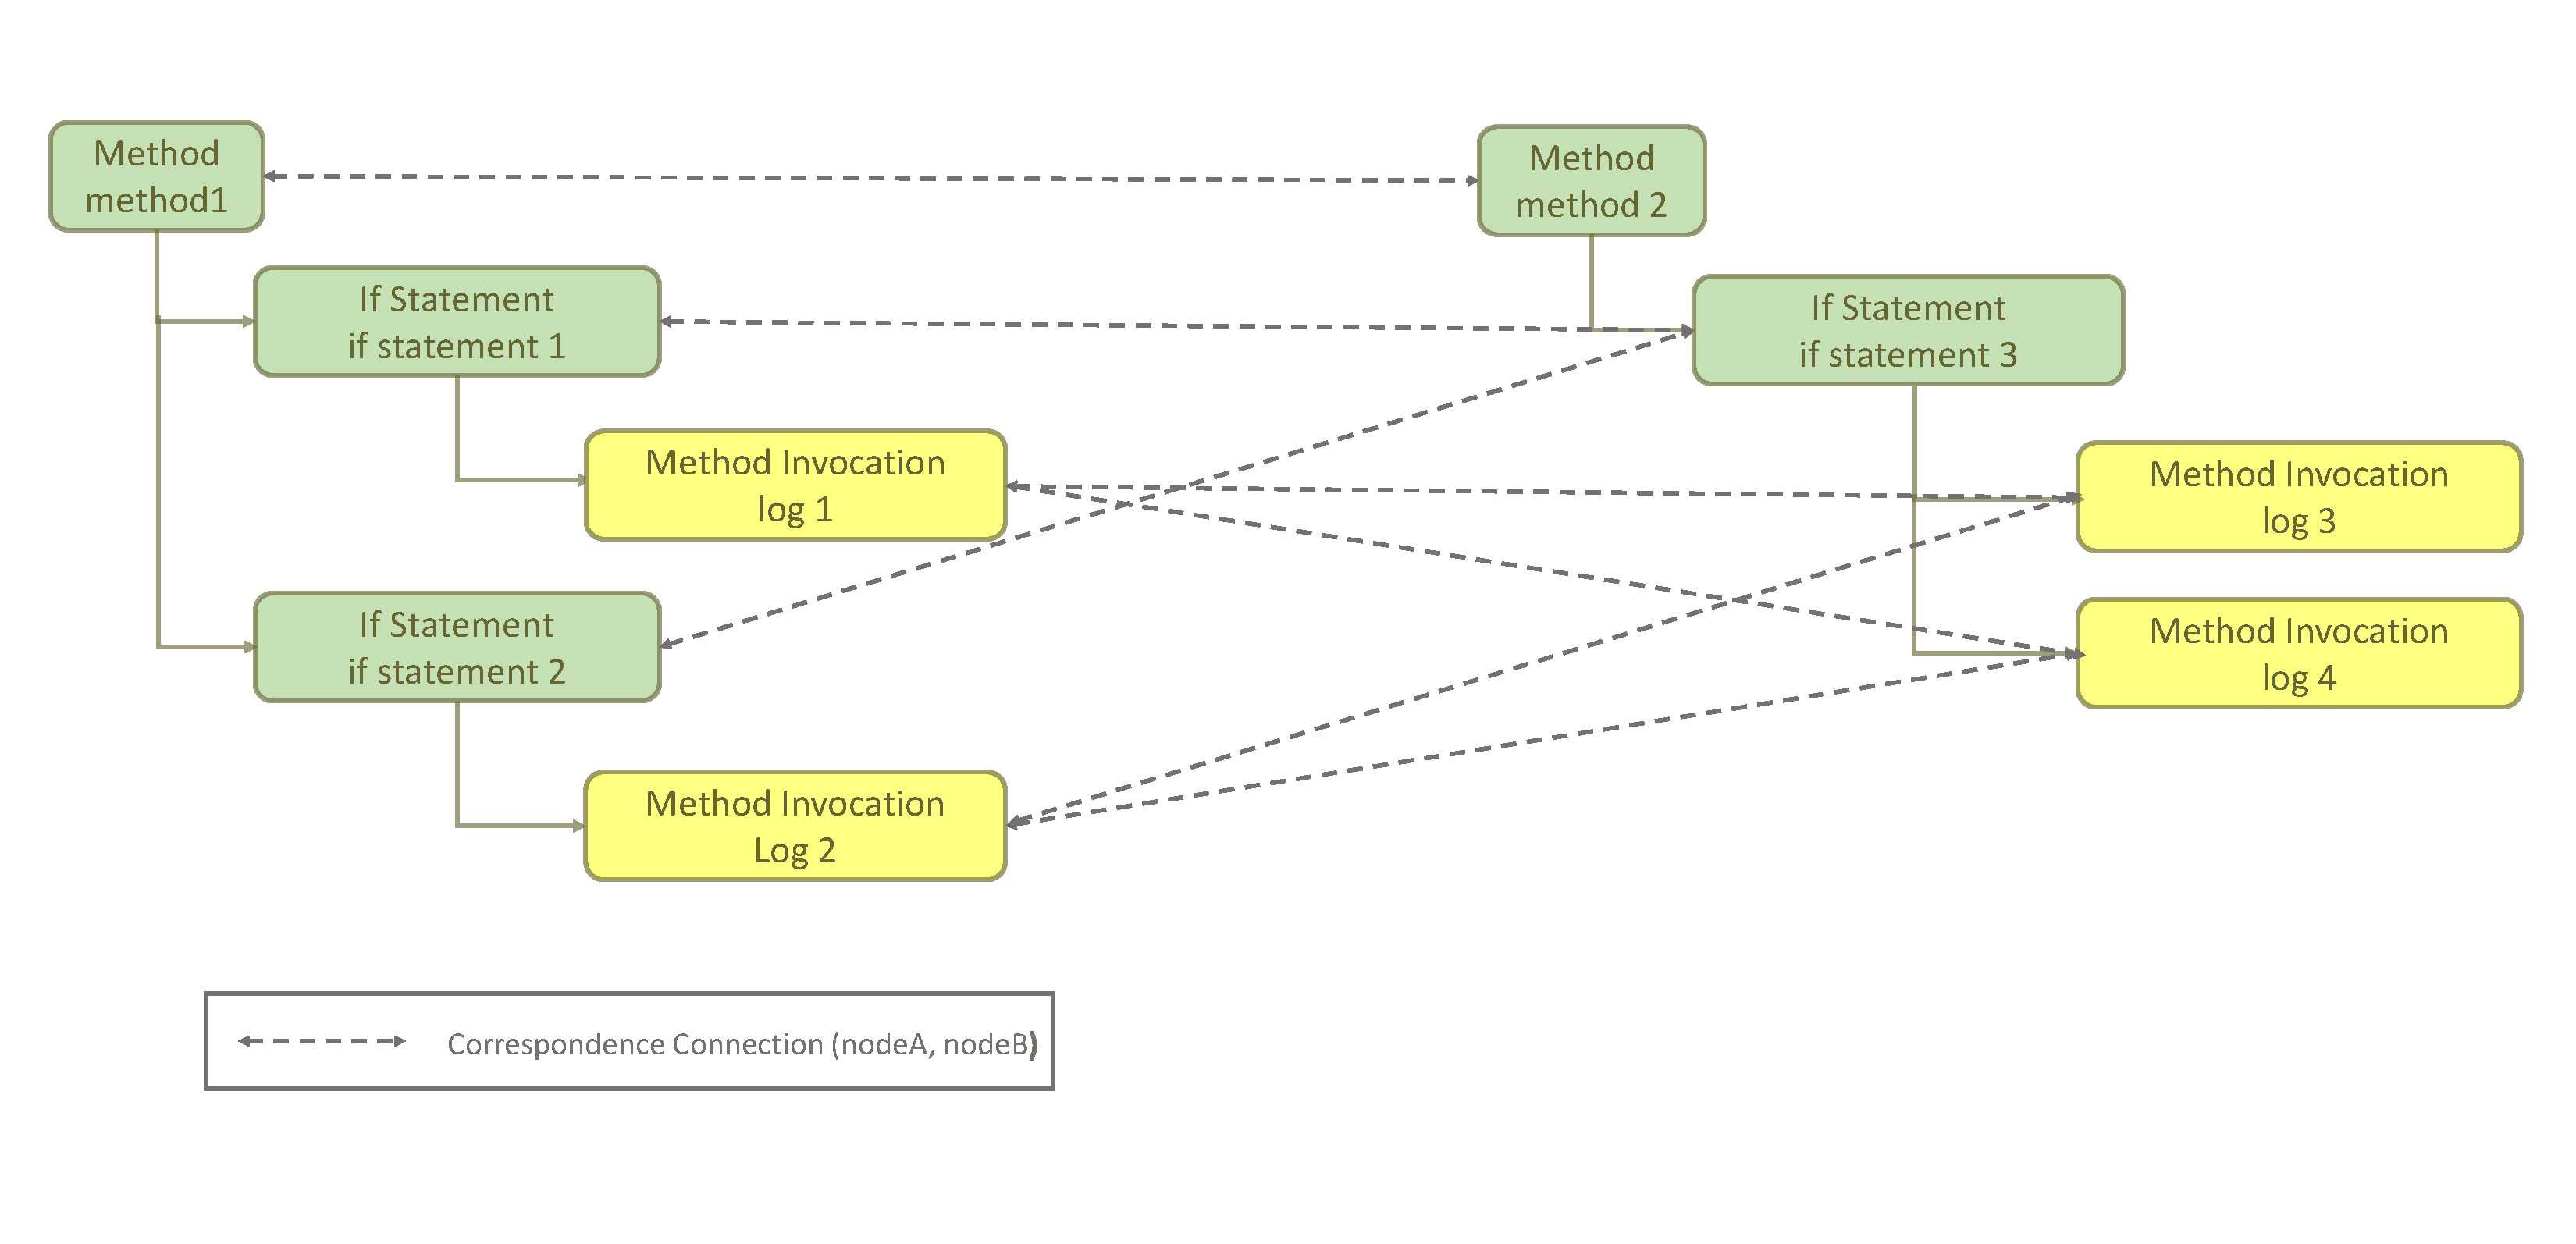
\includegraphics [width = \textwidth]{Drawing4/multipleLogging.pdf}
  \caption{Simple AUAST structure of examples in Figures~\ref{multiple1} and~\ref{multiple2}. Links between AUAST nodes indicate candidate structural correspondences detected by the Jigsaw framework.}
  \label{mast_1}
\end{figure}


\begin{figure} [H]
  \centering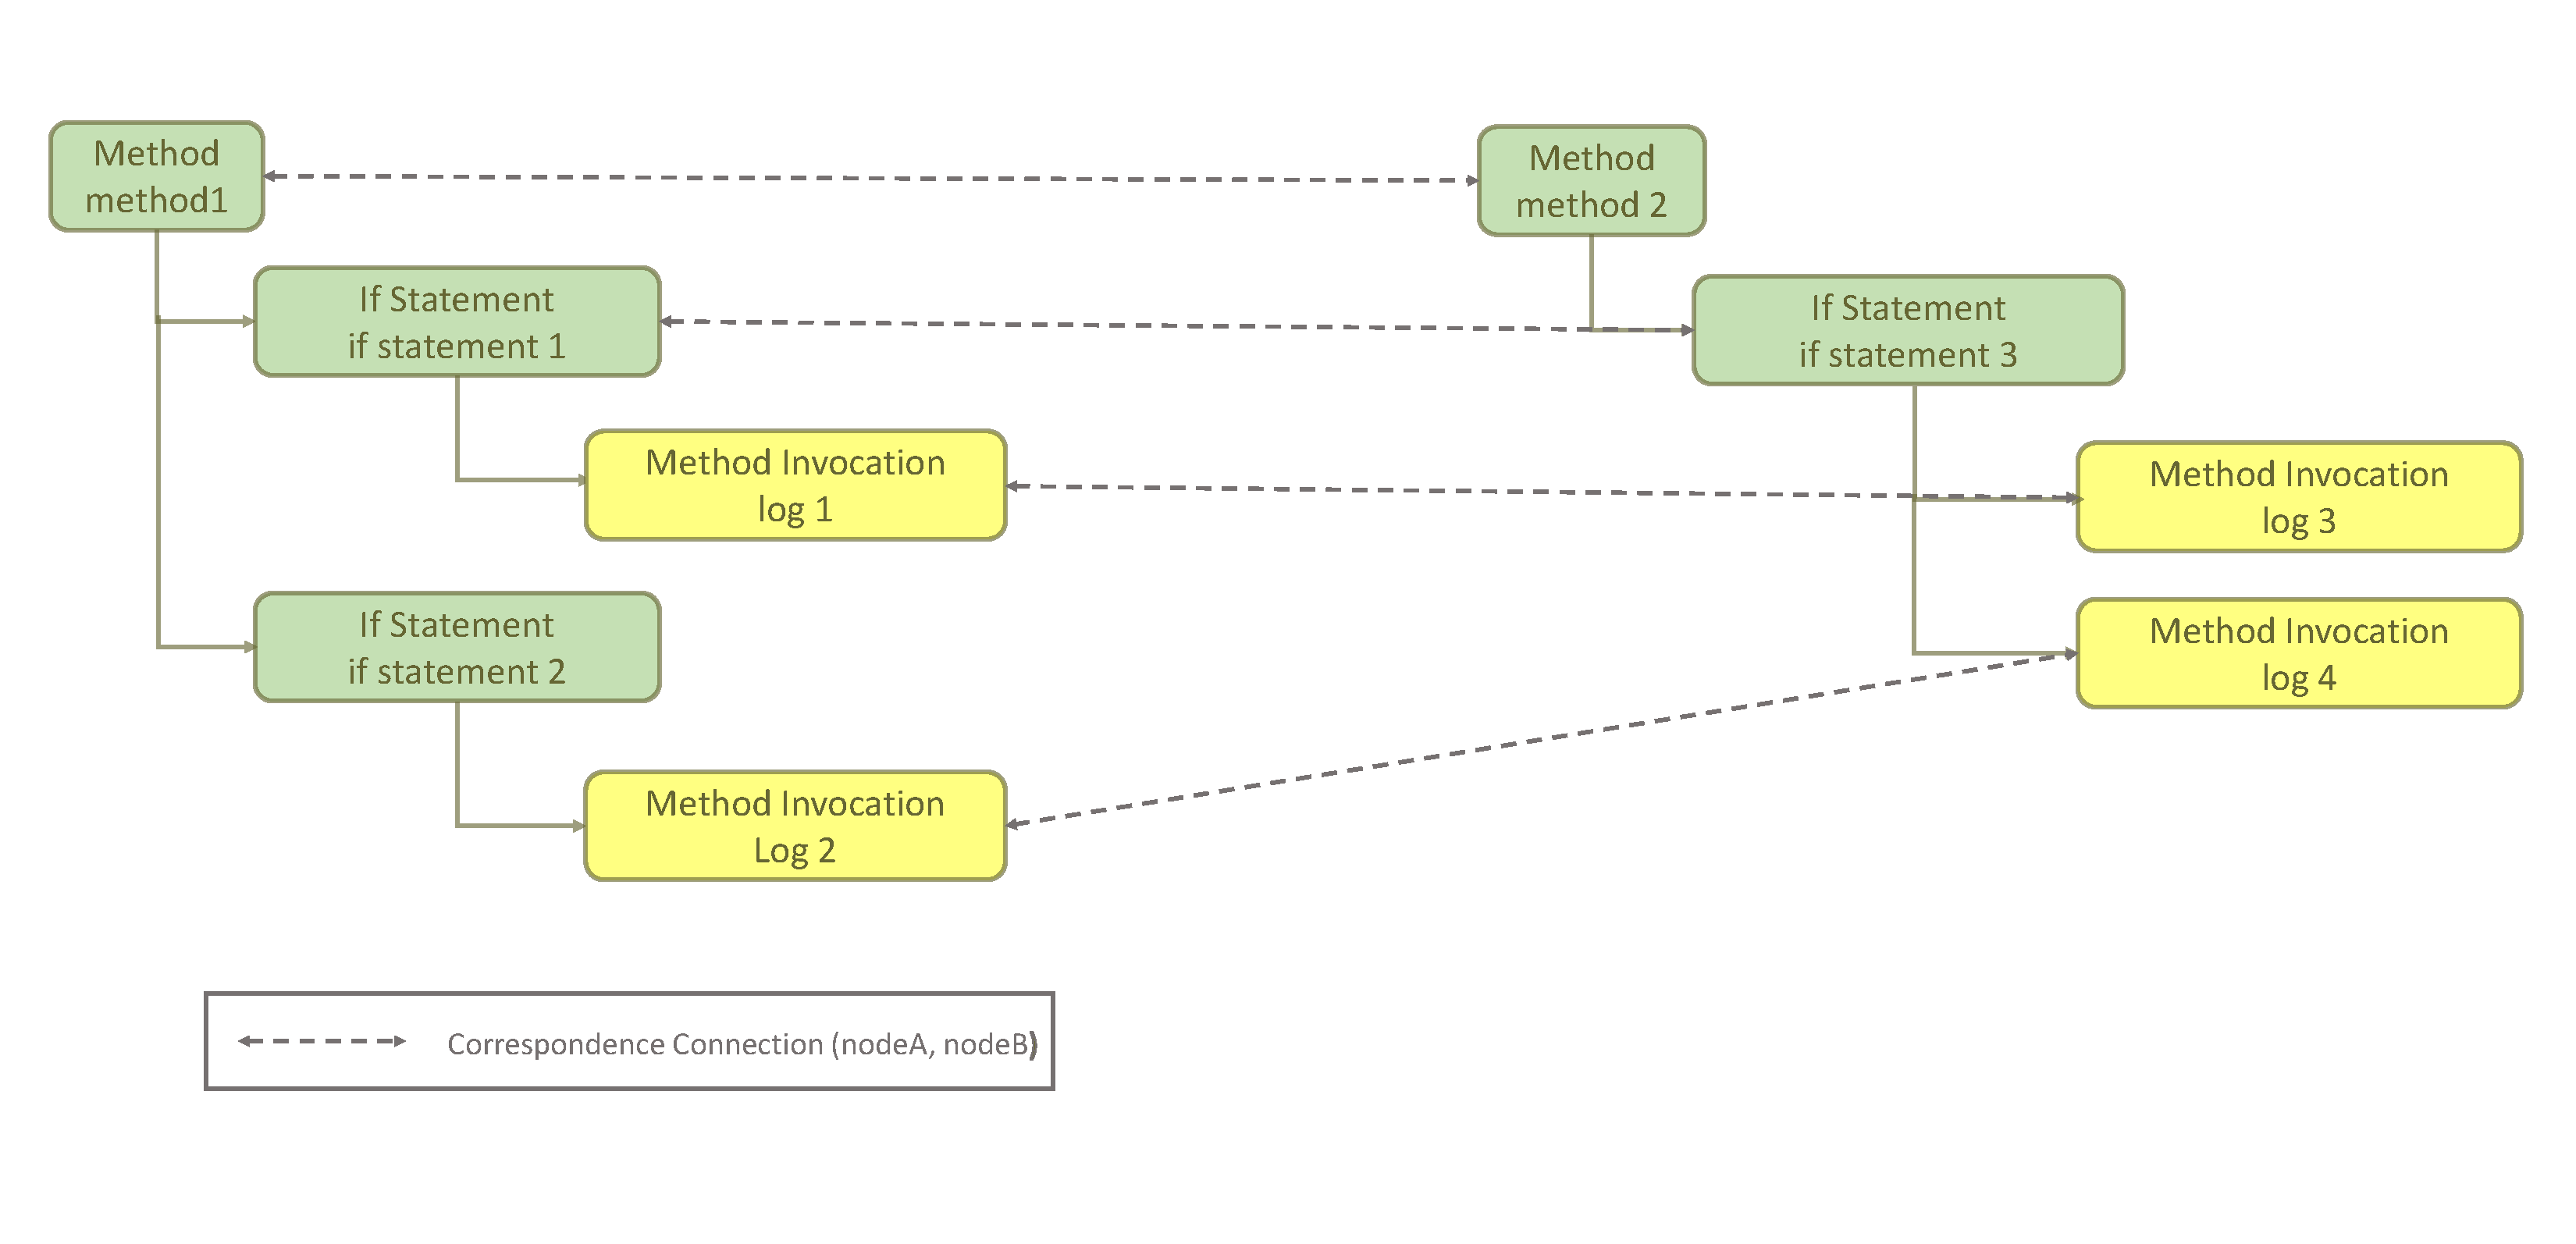
\includegraphics [width = \textwidth]{Drawing4/multipleLogging2.pdf}
  \caption{Simple AUAST structure of examples in Figures~\ref{multiple1} and~\ref{multiple2}. Links between AUAST nodes indicate structural correspondences selected as the best match using our greedy algorithm.}
  \label{m_ast2}
\end{figure}

To handle these cases, we can split them into more than one case, where each LJM contains only one logging call. To do so, we need to create a copy of LJM for each logging call by maintaining that logging call and removing the other ones. For example, we need to create two copies for each logged \name{Java} method of examples in Figures~\ref{multiple1} and~\ref{multiple2} as depicted in Figures~\ref{multiple1-one} and~\ref{multiple2-one}, respectively.
% thus constructing four possible anti-unifier for  possible combination and compute the similarity for each combination.
%We can split this case into more than one case, each with one logging statement in every seed. That is, for each case all the other logging statements should be deleted from seeds.  For example, imagine we have AST 1 and AST 2. AST 1 contains three logging calls and AST 2 contains two logging calls. As explained, we split AST 1 into AST 1a, AST 1b, and AST 1c. Also, we split AST 2 into AST 2a and AST 2b. We can split this case into 6 possible cases and create an anti-unifier for each possible combination and then compute a measure of similarity for each case. The best match for each log statement can be selected based on anti-unifier with the highest similarity amongst the other options.


\begin{figure}[H]
\def\baselinestretch{1}
\begin{lstlisting}

public void method1(){
	...
	if(condition1){
		Log.log();
	}
	...
	if(condition2){
		//removed
	}
	...
}

public void method1(){
	...
	if(condition1){
		//removed
	}
	...
	if(condition2){
		Log.log();
	}
	...
}

\end{lstlisting}
\caption{Create multiple copies of the LJM in Figure~\ref{multiple1} for each logging call.\label{multiple1-one}}
\end{figure}



\begin{figure}[H]
\def\baselinestretch{1}
\begin{lstlisting}
public void method2(){
	...
	if(condition3){
		//removed
		Log.log();
	}
	...
}

public void method2(){
	...
	if(condition3){
		Log.log();
		//removed
	}
	...
}

\end{lstlisting}
\caption{Create multiple copies of the LJM in Figure~\ref{multiple2} for each logging call.\label{multiple2-one}}
\end{figure}

%\section{An assessment of the anti-unifier-building tool}\label{anti-unifier-assessment}

\section{Evaluation} \label{anti-unifier-assessment}
%\subsection{Study 2: Detailed anti-unifier view}  \label{study2}
To assess the effectiveness of my anti-unification algorithm and the supporting tool, I conducted an experiment on the test suite described in Section~\ref{study1_setup}. %The anti-unifier-building tool is developed atop the correspondence tool to construct an anti-unifier from AUASTs of each LJM pair in our test suite.


\subsection{Setup}  \label{study2-setup}
In this study, we manually attempted to create the detailed anti-unifier view for each pair of LMs in the test suite (55 test cases in total). We first identified corresponding and non-corresponding \name{Java} elements for each LJM pair with a focus on preventing the correspondence of logging calls with anything else and then represented the anti-unifier in the detailed view (i.e., formatted as in Figure~\ref{fig:meth-anti-unifier}). We also computed the ratio of common \name{Java} elements in the detailed anti-unifier view to total number of \name{Java} elements of the two LMs to measure the similarity.
We also ran the anti-unifier-building tool on each pair of LMs to construct the detailed anti-unifier view for each pair with special attention to logging calls and to measure the similarity between the two LMs. Furthermore, we used \name{EclEmma}, which is a \name{Java} code coverage tool for \name{Eclipse}, to measure the test coverage. Test coverage is defined as a measure of the completeness of the set of test cases.


\begin{figure}
  \centering
  \begin{tabular}{cl}
    \toprule
    Test case & Logged methods \\
    \midrule

    \multirow{2}{*}{{1}}&\code{PluginJAR.generateCache()}\\
                         &\code{PluginJAR.generateCache()}\\
    \midrule

    \multirow{2}{*}{2}&\code{PluginJAR.generateCache()}\\
                         &\code{EditBus.send(..)}*\\
    \midrule

    \multirow{2}{*}{3}&\code{MiscUtilities.isSupportedEncoding(..)}\\
                         &\code{EditBus.send(..)}\\
    \midrule

    \multirow{2}{*}{4}&\code{EditBus.send(..)}\\
                         &\code{EditBus.send(..)}*\\
    \midrule
    \multirow{2}{*}{5}&\code{EditBus.send(..)}*\\
                         &\code{EditAction.Wrapper.actionPerformed(..)}\\
    \midrule

    \multirow{2}{*}{6}&\code{EditBus.send(..)}*\\
                         &\code{BufferHistory.RecentHandler.doctypeDecl(..)}\\
    \midrule

    \multirow{2}{*}{7}&\code{EditAction.Wrapper.actionPerformed(..)}\\
                         &\code{JARClassLoader.loadClass(..)}\\
    \midrule

    \multirow{2}{*}{8}&\code{EditAction.Wrapper.actionPerformed(..)}\\
                         &\code{VFS.DirectoryEntry.RootsEntry.rootEntry(..)}\\
    \midrule

    \multirow{2}{*}{9}&\code{PluginJAR.generateCache()}\\
                         &\code{BufferHistory.RecentHandler.doctypeDecl(..)}\\
    \midrule

    \multirow{2}{*}{10}&\code{VFS.DirectoryEntry.RootsEntry.rootEntry(..)}\\
                         &\code{ServiceManager.loadServices(..)}\\
    \bottomrule

  \end{tabular}
  \caption{10 sample logged \name{Java} method pairs used as test cases; all are contained in the \protect\name{org.gjt.sp.jedit} package with the exception of cases 8 and 10 that are in the \protect\name{org.gjt.sp.jedit.io} package.}
  \label{study2_test_cases}
\end{figure}





%The view would be in the form depicted in ..

\subsection{Results}  \label{study2-results}
We present the results of our analysis for a subset of 10 test cases (see Table~\ref{study2_test_cases}) in Table~\ref{study2_test_cases_results}. The analysis of the output has been divided into two categories: correspondence and similarity. "Correspondence" refers to the number of corresponding lines-of-code (LOC) detected by our tool that were found to be corresponded by our manual examination as well, and the number of LOC detected as corresponded by our tool but were not found to be corresponded in our manual inspection. We also present the percentage of the correct corresponding LOC to the total number of LOC of the two LMs. "Similarity" refers to the similarity that is computed based on the the detected correspondences. It is calculated using both our tool and manual experiment.



In case 8, the \code{rootEntry(..)} method contains a nested \code{if}-statement enclosing a logging call and the \code{actionPerformed(..)} method contains an \code{if}-statement enclosing another logging call. The analysis showed that a correct correspondence was detected between the inner \code{if}-statement inside the nested \code{if}- and the single \code{if}-statement. Cases~3 and~10 contain statements that are not found to correspond by our tool even though correspondences exist. For example, in case 3, the \code{isSupportedEncoding(..)} method contains an assignment statement enclosed by an \code{if}-statement that does not have any correspondences and the \code{send(..)} method contains another assignment statement inside a \code{for}-statement without any correspondences as well. However, no correspondence was detected between the two assignment statements since their parent nodes do not correspond.
\begin{figure}
  \centering
  \begin{tabular}{|c|c|c|c|c|c|}
    \hline
    \multirow{2}{*}{Test case}&\multicolumn{2}{c|}{Correspondence}&\multicolumn{2}{c|}{Similarity}\\
    \cline{2-5}
    &Correct (\%)&Incorrect&human&tool\\
    \hline
    1&104(100)&0& 1.0 & 1.0\\
    \hline
    2&8(100)&0& 0.13& 0.13\\
    \hline
    3&6(85)&1&0.19& 0.16\\
    \hline
    4&4(100)&0&0.29 &0.29\\
    \hline
    5&5(100)&0&0.21 &0.21\\
    \hline
    6&3(100)&0&0.2 &0.2\\
    \hline
    7&5(100)&0&0.11 &0.11\\
    \hline
    8&7(100)&0& 0.1&0.1\\
    \hline
    9&3(100)&0&0.03&0.03 \\
    \hline
    10&14(87)&2&0.27 &0.22\\
    \hline

  \end{tabular}
  \caption{Results of constructing anti-unifiers with a focus on logging calls for the 55 test cases.}

  \label{study2_test_cases_results}
\end{figure}

The results of the pairwise comparison between LMs of the test suite is visualized in Figure~\ref{fig:au_graph}. Our anti-unifier-building tool succeeded in detecting correspondences with special attention to anti-unifying logging calls and calculating pairwise similarities in 48 out of 55 test cases. In addition, the test coverage of our test cases was measured 82\% using \name{EclEmma}.

\begin{figure} [H]
  \centering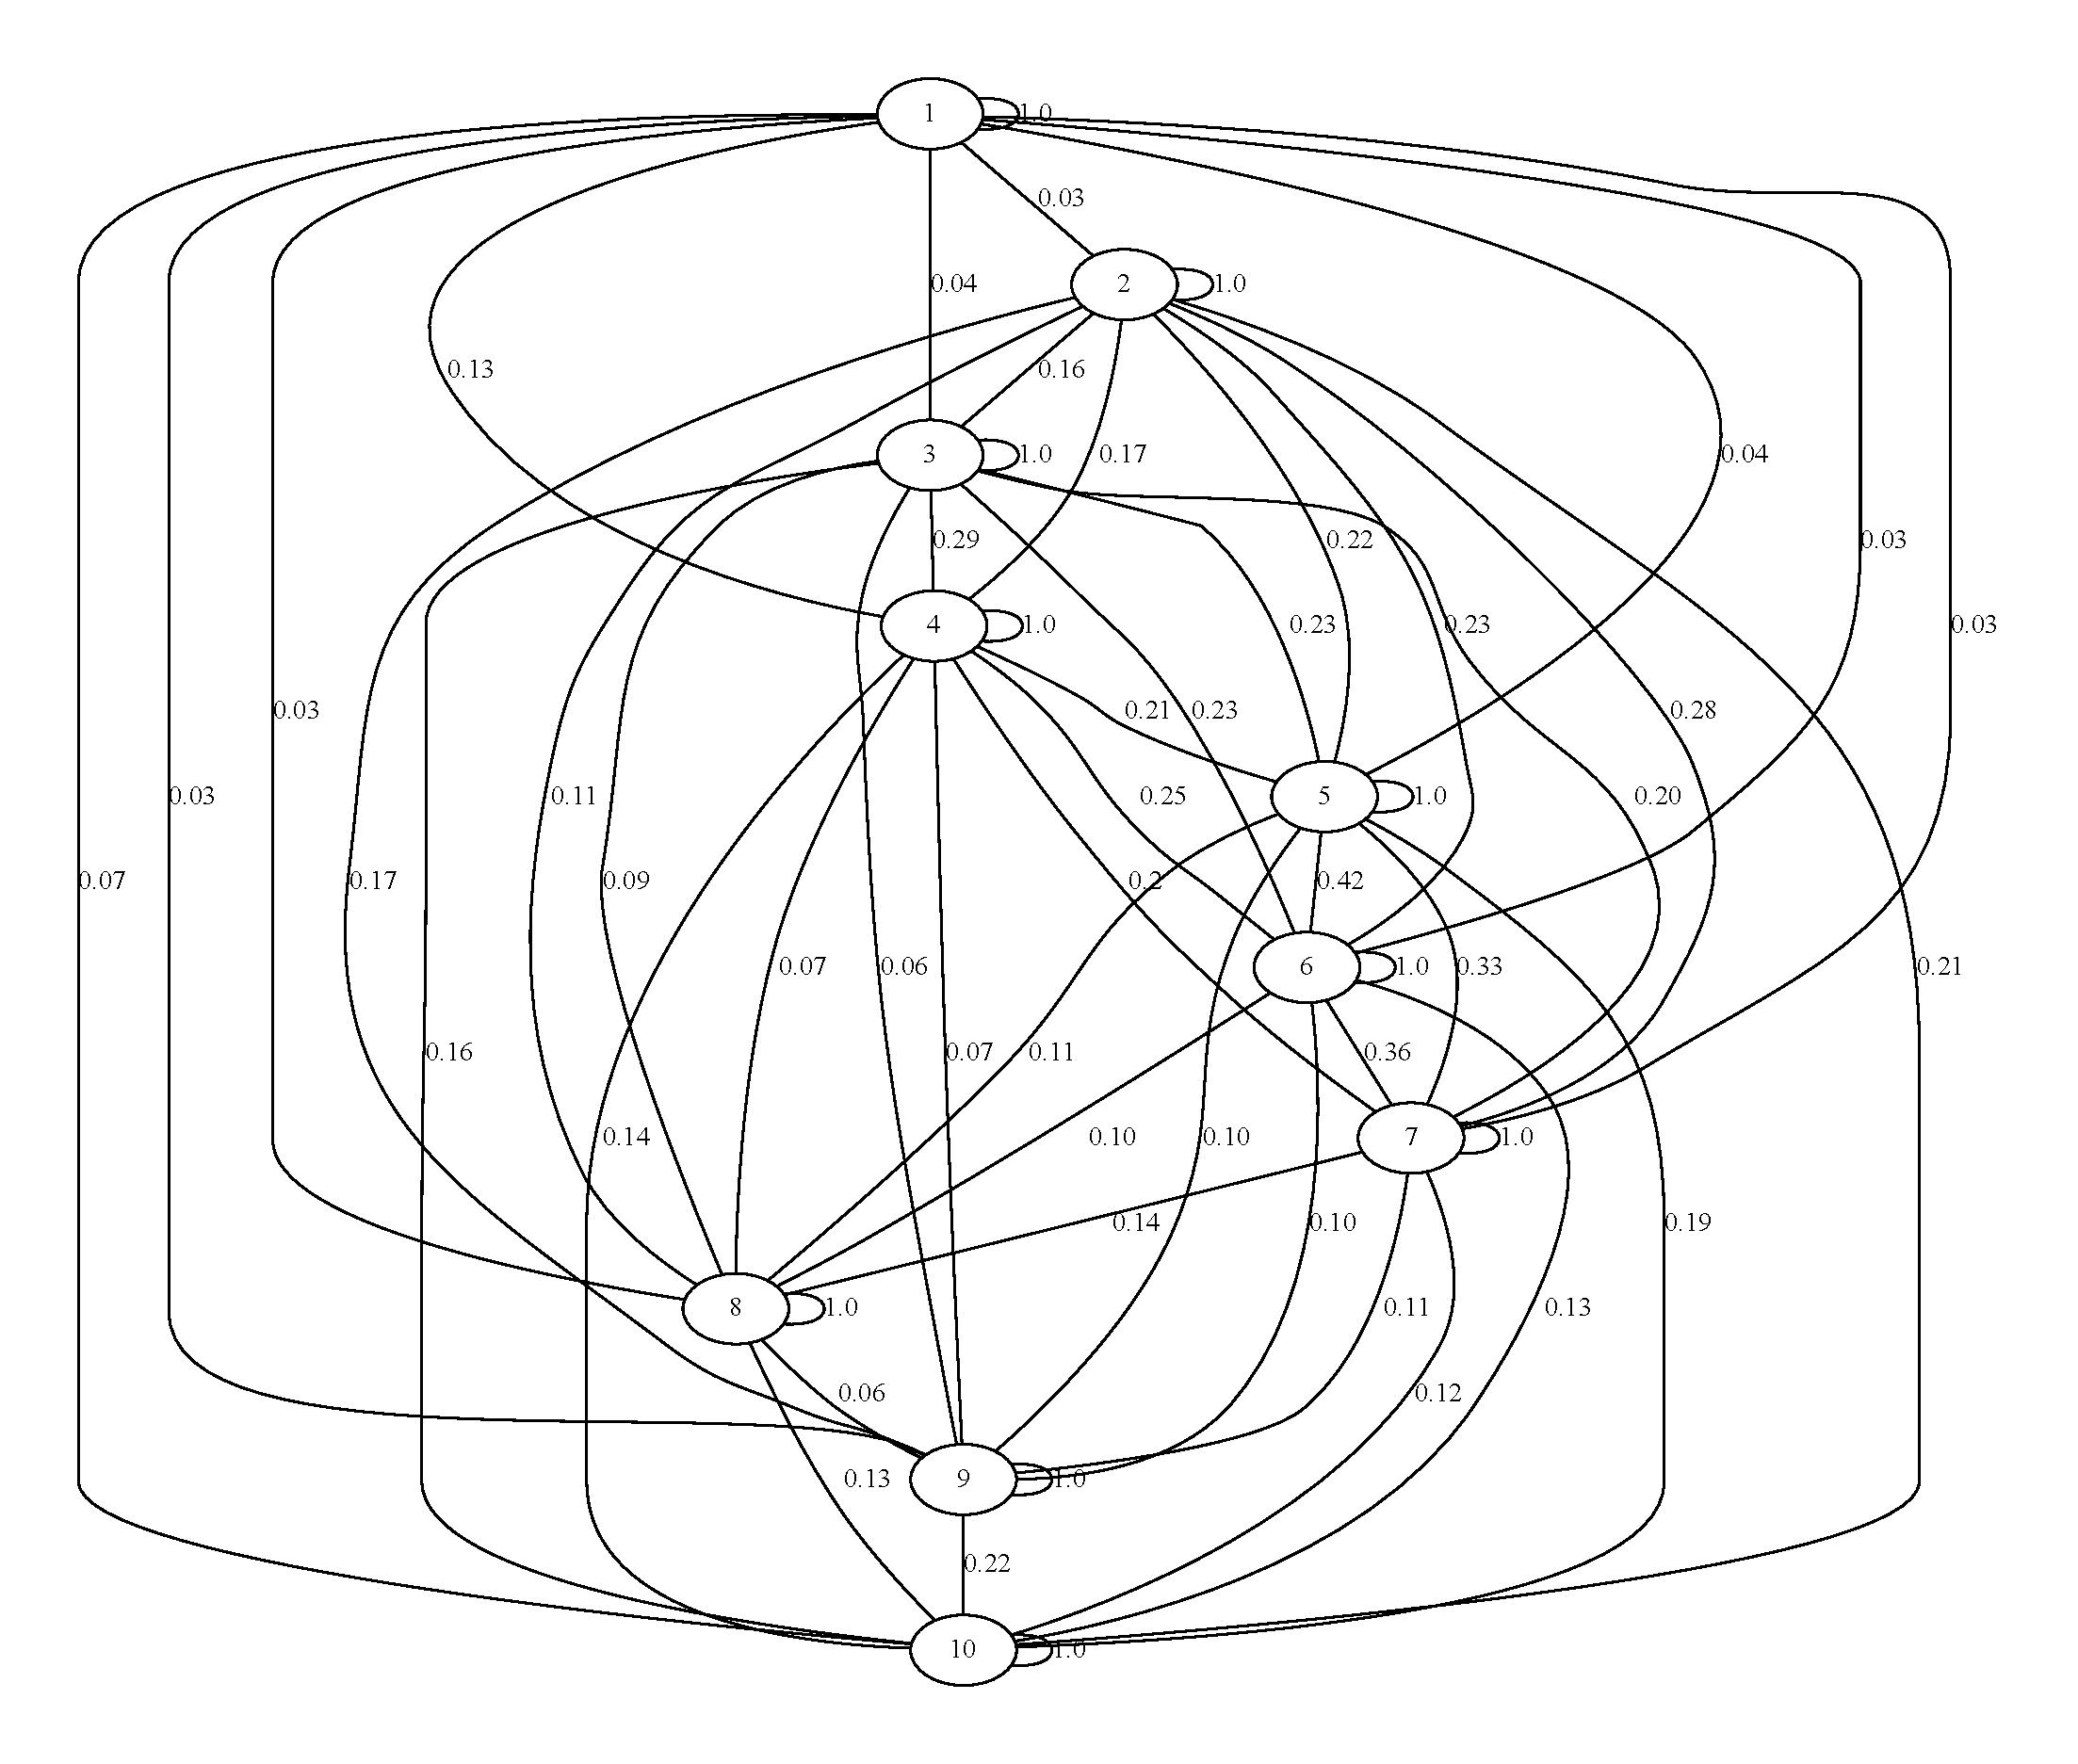
\includegraphics [width = \textwidth]{graphviz/au.pdf}
  \caption{A similarity graph representing pairwise similarities calculated by our tool between LMs shown in Table~\ref{table:ljms}.}
  \label{fig:au_graph}
\end{figure}




\section{Summary} \label{meth1-summary}
I have presented an approach for constructing a generalization from AUASTs of two LMs with special attention to logging calls via structural correspondence. This approach proceeds in three steps. First, several constraints have been applied on the selection of correspondences to prevent anti-unifying log method invocation nodes with any other types of nodes. Second, an approximation technique is employed to find the best correspondence for each AUAST node. Third, the anti-unification of two AUASTs is performed through the application of higher-order modulo theories over the AUAST structures. Furthermore, a measure of similarity has been developed that would provide us with useful information for the clustering phase.

An experimental study was conducted to evaluate the effectiveness of our anti-unification algorithm and the tool support in constructing an anti-unifier from AUASTs of each LJM pair in our test suite with a focus on logging calls and measuring similarity between them.



%This approach is implemented as an Eclipse plug-in which given two logged Java methods utilizes the Eclipse JDT framework to extract their ASTs. In order to be able to apply HOAUMT, we extended the AST structure to a higher-order structure, called AUAST, that would allow the insertion of variables in place of any nodes. We then applied the Jigsaw framework to identify potential correspondences between the two AUASTs and greedily determines the best correspondence for each node with the highest Jigsaw similarity.  Moreover





\addtocontents{toc}{\protect\addvspace{10pt}}
\chapter{Clustering}  \label{clustering}
In Chapter~\ref{ch4}, I described my anti-unification algorithm to construct an anti-unifier from the AUASTs of a pair of LMs, paying special attention to log statements. Recall that the general point of this study is to provide a description of where log statements happen in source code by constructing structural generalizations that represent the detailed commonalities and differences between the AUASTs of LMs. To this end, I should develop an algorithm that:
\begin{itemize} [leftmargin=.5in]
\item classifies the methods showing different ways of locating log statements into separate clusters; and
\item abstracts the AUASTs of LMs of each group into a structural generalization representing the similarities and differences between them.
\end{itemize}

In Section~\ref{m-clustering-alg}, I describe a modified version of an agglomerative hierarchical clustering algorithm I developed for my application. The clustering algorithm is a bottom-up approach that starts with singleton clusters, each contains one AUAST, and then it repeatedly merges the closest clusters that are the ones with maximum similarity between their AUASTs. To evaluate my approach, I have implemented the clustering tool (Section~\ref{clusteringTool}) and conducted an experimental study through the application of it on the test suite introduced in Section~\ref{study1_setup}. I will describe my experimental study and discuss the results in Section~\ref{clustering-assessment}.
% I developed for my application.?

%Therefore, before the use a clustering algorithm to classify a set of AUASTs, I need to first
%Clustering is the classification of a collection of unlabelled data items into meaningful groups \cite{jain1999data}, where category labels are obtained from the similarities between data items.


\section{Modified agglomerative hierarchical clustering algorithm} \label{m-clustering-alg}
%To develop a measure of similarity between AUASTs, I used the similarity function described in Section~\ref{meth-similarity}.
%unsupervised???
%by computing pairwise similarities between cluster pairs?
Clustering is an unsupervised machine mining technique that aims to organize a collection of data into clusters, such that intra-cluster similarity is maximized and the inter-cluster similarity is minimized \cite{karypis1999chameleon,grira2004unsupervised}. 
To perform clustering on a set of AUASTs of LMs, I developed Algorithm~\ref{modified-agglomerative}, which is a modified version of the agglomerative hierarchical clustering algorithm. The clustering algorithm is a bottom-up approach that starts with singleton clusters, each contains one AUAST (Line~1), and then it creates a similarity matrix by computing pairwise similarities between cluster pairs (Line~2). This step requires defining a notion of cluster similarity. As I intend to construct an anti-unified AUAST for each cluster, the similarity between two clusters is measured based on the similarity between their AUASTs.
\RW{Add to bib},
\RW{Note: you don't describe this tool in any detail.  I am assuming it is straightforward.}\NZ{ Yes, It is straightforward. I just implemented the algorithm I described here.}
\RW{Why did you do it manually?  You are assuming that your manual approach represents the ground truth, which may not be true; this is a point for discussion in threats to validity.}\NZ{ I changed the way I evaluated the clustering algorithm, and defined some measurements that can be calculated using equations.}



In general, this hierarchical algorithm employs a $n \times n$ similarity matrix for a set of $n$ AUASTs, where an element in row $i$ and column $j$ represents the similarity between the $i^{\text{th}}$ and the $j^{\text{th}}$ clusters. The similarity between two clusters is defined as the similarity between their AUASTs, which is computed through the algorithm described in Section~\ref{meth-similarity}. However, there are some cases in which the anti-unification of the AUASTs of two clusters does not allow the anti-unification of log statements with one another, since the structures enclosing them are not corresponded. To handle these cases, I adjusted the similarity value between the two clusters to zero. Then the algorithm repeatedly merges the closest clusters that are the ones with maximum similarity between their AUASTs, and update the similarity matrix by computing the similarity between the new cluster and the old clusters (Lines~5--6). The merge and update steps are repeated until the similarity between closest clusters becomes below a predetermined threshold value (Line~7). Through informal examination, I have found that a threshold value of 0.05 gives the reasonable results, as it allows the classification of methods showing different ways of locating log statements in separate clusters. I also used the anti-unification algorithm described in Section~\ref{meth-antiUnifier} to construct an anti-unifier for each cluster.
%threshold???
%allows? the classification of methods showing different ways of locating log statements in separate clusters?

 %to prevent the combination of a cluster pair when the usage of logging is different, I adjusted the similarity between them to zero. they should be in separate clusters.


\begin{algorithm}
\caption{Modified agglomerative hierarchical clustering algorithm.} \label{modified-agglomerative}
\begin{algorithmic}[1]
\State Start with singleton clusters.
\State Compute a similarity matrix.
\Repeat
\State Find the closest clusters.
\State Merge the closest cluster pair and replace the original clusters with a new cluster containing the anti-unifier of their AUASTs.
\State Update the similarity matrix by computing the similarity between new cluster and all remaining clusters.
\Until the similarity between closest clusters becomes below a predetermined threshold value.
\end{algorithmic}
\end{algorithm}



Figure~\ref{fig:overview2} illustrates the clustering process for a sample set of 5 AUASTs using the initial similarity matrix depicted in Figure~\ref{matrix}. In the first and second iterations, clusters 1 and 2, and clusters 4 and 5 are selected as the closest clusters, merged, and replaced by clusters 6 and 7, respectively. If threshold value is determined as Threshold $A = 0.20$, the process should be terminated at this step, as the similarity between the closest clusters (clusters 3 and 6) is below this threshold; otherwise, these clusters should be merged and replaced by cluster 8. However, the similarity between AUASTs of clusters 7 and 8 is zero, and thus they should not be merged with each other. 
%THRESHOLD B??



\begin{figure} [H]
\begin{displaymath}
    similarity = \left[
        \begin{matrix}
        1.00 &  &  &  &   \\
0.28 & 1.00 &  &  &  \\
0.12 & 0.17 & 1.0 &  &  \\
0.00 & 0.00 & 0.00 & 1.0 &  \\
0.00 & 0.00 & 0.00 & 0.21 & 1.00
        \end{matrix}   \right]
\end{displaymath}
 \caption{The similarity matrix for a sample set of 5 AUASTs.}
  \label{matrix}
\end{figure}




\begin{sidewaysfigure} [p]
  \centering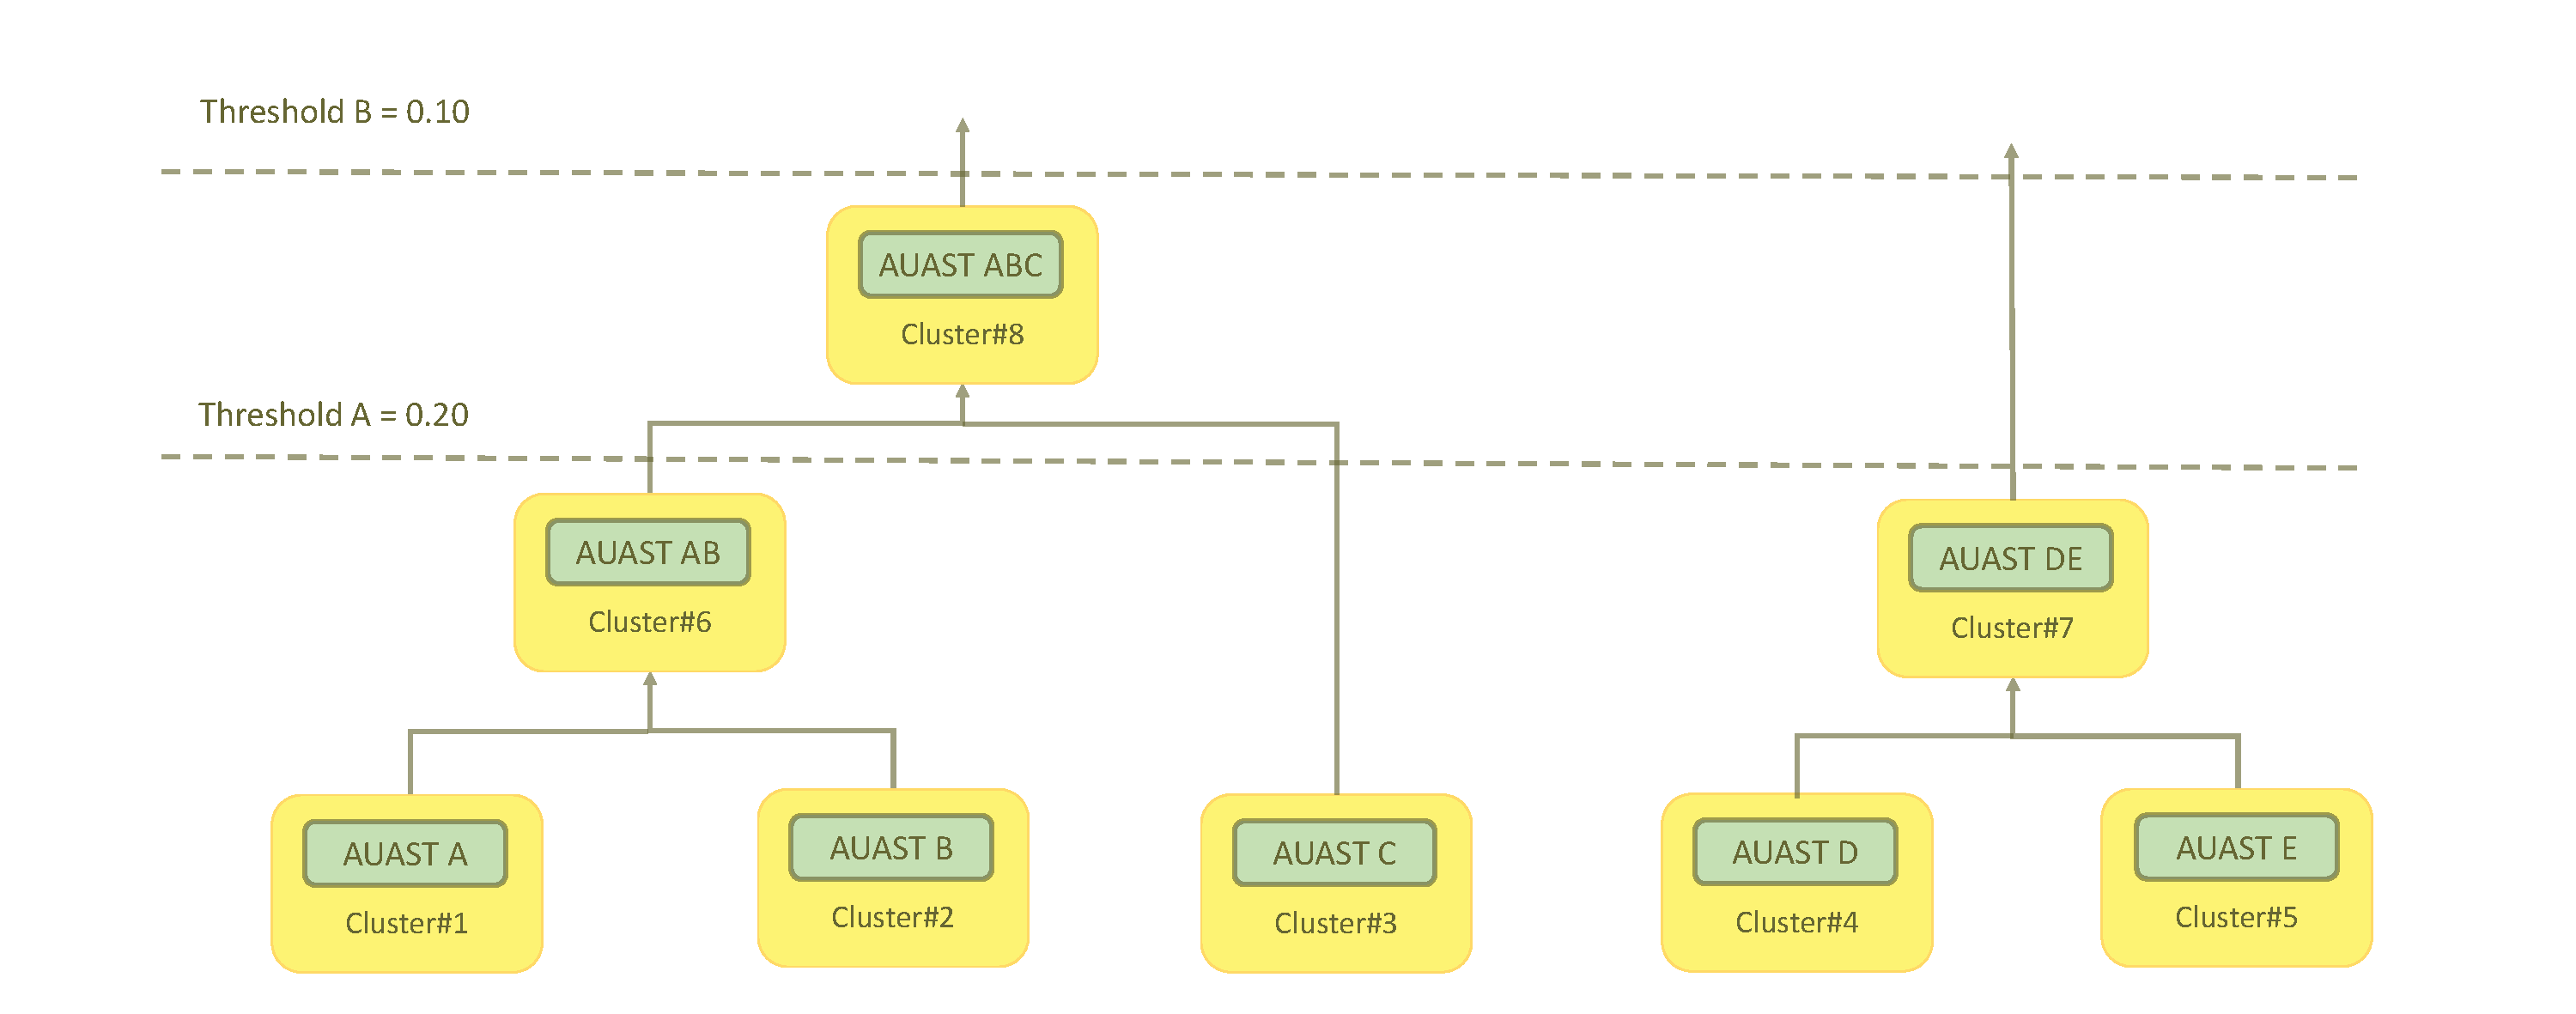
\includegraphics [width = \textwidth]{Drawing4/overview2.pdf}
  \caption{The modified agglomerative hierarchical clustering process on a sample set of  5 AUASTs using the initial similarity matrix shown in Figure~\ref{matrix}. The threshold value indicates the number of resulting clusters.}
  \label{fig:overview2}
\end{sidewaysfigure}

%\section{An assessment of the Clustering tool} \label{clustering-assessment}
%To evaluate the quality of a clustering algorithm
\section{Evaluation} \label{evaluation}
To evaluate the clustering approach, I have implemented a tool and conducted an experiment on the set of AUASTs of LMs described in Table~\ref{table:ljms}. The clustering tool is an Eclipse plug-in built atop the anti-unifier building tool that inputs a set of AUASTs of LMs extracted from the source code, applies the clustering algorithm on them, and outputs an anti-unifier for each cluster. Then, I have developed some measurements to assess the goodness of the resulting clusters. Recall that the goal is that the objects within a cluster should be similar to one another and dissimilar from the other clusters \cite{}. The measures of cluster evaluation can be divided into two types:
\begin{itemize} [leftmargin=0.4in]
\item \emph{Cluster cohesion:} which determines how closely related the objects within a cluster are. In this experiment, the cohesion of each cluster can be defined as the sum of the similarities between the AUAST of each LM in the cluster and the AUAST of the cluster anti-unifier.
\item \emph{Cluster separation:} which determines how isolated or well-separated a cluster is from the other clusters. In this experiment, the separation between two clusters can be defined as the similarity between the two cluster anti-unifiers.
\end{itemize}

\subsection{Setup}  \label{study3-setup}
%I manually attempted to perform the hierarchical clustering on the set AUASTs of LMs in the test suite and constructed the detailed anti-unifier view for each cluster. Anti-unifiers were discarded when the anti-unification of LMs did not allow the anti-unification of logging calls with one another, as the Java elements enclosing them were not found to be corresponded. I also measured the level of similarity between AUASTs in each cluster by computing the ratio of common Java elements in the detailed anti-unifier view to the total number of Java elements of all AUASTs in that cluster. I also ran the clustering tool on the set of AUASTs to classify them using the similarity measurement.

I ran the clustering tool on the set of AUASTs of LMs of the test suite. To evaluate the quality of the resulting clusters, I computed the cohesion of each cluster and the separateness between each cluster pair using the following equations, respectively:


\begin{tabular}{c}
  $cohesion(C_i) = \frac{ \sum_{x \in C_i} similarity(x,antiUnifier[C_i] )}{N_i}$  \\  
\end{tabular}

\begin{tabular}{c}
  $separateness(C_i,C_j) =  similarity(antiUnifier[C_i],antiUnifier[C_j])$ \\ \\
\end{tabular}

Where $C_i$ is the  $i^{\text{th}}$ cluster, and $N_i$ is the cluster size of cluster ${C_i}$. 


\subsection{Results}  \label{study3-results}

%I present the results of my analysis in Table~\ref{results_clustering}. The analysis of the output has been divided into three categories: correspondence, similarity, and separateness. The analysis of correspondence and similarity was described in Section~\ref{study2-results}. "Separateness" refers to my tools' ability to cluster Java method with different usages of log statements into separate groups, and the ones with similar usages of log statements into the same cluster.

The cohesion and separateness for the resulting clusters are presented in Tables~\ref{results_clustering_cohesion} and~\ref{results_clustering_separateness}, respectively.


\begin{figure} [H]
  \centering
  \begin{tabular}{ccc}
    \toprule
    {Cluster}&{$N_i$}&{Cohesion}\\
    
    \midrule
    1&4& \\
    \midrule
    2&3&\\
    \midrule
    3&3& \\
 	\bottomrule
  \end{tabular}
  \caption{The cohesion of the clusters produced by applying the clustering tool to the test suite described in Table~\ref{table:ljms}}
  \label{results_clustering_cohesion}
\end{figure}



\begin{figure} [H]
  \centering
  \begin{tabular}{cc}
    \toprule
    {Cluster}&{Separateness}\\
    \midrule
    1-2& \\
    \midrule
    1-3& \\
    \midrule
    2-3& \\
 	\bottomrule
  \end{tabular}
  \caption{The separateness between each cluster pair produced by applying the clustering tool to the test suite described in Table~\ref{table:ljms}}
  \label{results_clustering_separateness}
\end{figure}

Clusters 1, 2, and 3 contain logged methods of cases (1, 3, 5, 8), (2, 9, 10), and (4, 6, 7), respectively. 
The separation results show that our algorithm was able to generate well-separated clusters.
The cohesion results are above...  for all the resulting clusters which indicates that the LMs in the same cluster are closely related to one another. In general, this experiment shows that our algorithm results in good quality clusters in terms of cohesion and separateness measurements.
%, as detected by my manual inspection.
%, as the LMs within each cluster used similar ways of locating log statements and dissimlar ways compared to the other Lms in the other clusters.   


%?????
%The clustering tool succeeded in detecting the separateness amongst AUASTs of test cases correctly. Clusters 1, 2, and 3 contain logged methods of cases (1, 3, 5, 8), (4, 6, 7), and (2, 9, 10), respectively, as detected by my manual inspection. It also successfully calculated the similarity between LMs of 2 clusters out of 3. In Cluster 2, the error in detecting correspondences originated from the previous study and propagated to the clustering study. However, it is trivial (0.01) and would have a low impact on our final results.
%between the LMs of our test suite.

\section{Summary} \label{meth2-summary}
I have presented a modified version of the agglomerative hierarchical clustering algorithm to classify logged methods showing different usages of log statements into separate clusters. This algorithm is implemented as an Eclipse plug-in that takes a set of AUASTs of LMs, clusters them by computing the pairwise similarities between AUASTs, and generates an anti-unifier for each cluster. Furthermore, an experimental study was conducted to validate the effectiveness of my clustering algorithm and the tool support on a test suite.





\addtocontents{toc}{\protect\addvspace{10pt}}
\chapter{Characterization Study}\label{discover}\label{eval}

To characterize the location of log statements in source code, I conducted an experimental study that addresses the following research questions:

\begin{itemize} [leftmargin=.5in]
\item \textsc{RQ1: }\emph{``Is it possible to find patterns of where log statements occur in source code?''} I aim to investigate whether there are clusters containing a large number of LMs. This suggests that there might be common ways of locating log statements in source code.

\item \textsc{RQ2: }\emph{``What common structural characteristics do logged methods have?''} I conducted a manual analysis on the logging usage schemas (LUSs) produced by \tool{ELUS} to identify the common structural characteristics of LMs in each cluster.
\end{itemize}


\section{Experiment}  \label{setup-characterization}
%\subsection{Setup}  \label{setup}
In this experiment, I will analyze logging usage of four popular open-source software systems: \name{Apache Tomcat}, \name{Hibernate ORM}, \name{Apache Camel}, and \name{Apache Solr}. Each system is written in the Java programming language and they all utilize the same logging framework, \name{Apache log4j}. I decided to study the usage of \name{log4j} statements in these systems, as \name{Apache log4j} is ranked as the most commonly used logging package for Java\footnote{\url{https://en.wikipedia.org/wiki/Java_logging_framework}}. The studied systems are from different application domains: \name{Apache Tomcat} is a Java Servlet; \name{Hibernate ORM} is an object relational-mapping framework; \name{Apache Camel} is a rule-based routing and mediation engine; and \name{Apache Solr} is an enterprise search platform. I chose these systems as my study subject due to their popularity in their area of application (7000+ commits to the \name{GitHub} repository) and their long history of development (9 to 13 years). Table~\ref{table:CSts} represents the details about these software systems. I also decided to exclude the \name{log4j} statements at the \name{trace} and \name{debug} verbosity levels, as they are usually used by developers only during the software development phase. I believe that studying these systems could give us an insight about logging usage in real-world applications.


%I only examined the log statements from the \name{Apache log4j} framework, and


\begin{figure} [H]
  \centering
  \begin{tabular}{llcccc}
    \toprule
    \textbf{Software system}  & \textbf{Description}   & \textbf{Version} & \textbf{Start time} & \textbf{LOC} & \textbf{Log statements} \\ \hline
    {Tomcat} & Server  & 9.0.11& 2003 &306,704 &  3,117 \\ \hline
{Hibernate ORM} & Framework & 4.2.23 & 2004 & 509,734 & 1,939 \\ \hline
    {Camel} &  Middleware & 2.18.0 &  2007 &120,528 & 2,177 \\
    \hline
    {Solr} &  Platform  & 6.2.1 &  2007 & 128,824 & 2,319 \\
%{OpenMeetings} & Web Conferencing & & 2.0 &38K &3506 \\ \hline
 %   {QuickFIX/J} & Engine & 1.6 & 48K & 2958 \\
   % \bottomrule
    \toprule
  \end{tabular}
   %\caption{Details of the four open-source software systems that make use of the {Apache log4j} logging framework.}
    \caption{Summary of the four software systems used in the characterization study.}
\label{table:CSts}
\end{figure}


My proof-of-concept implementation takes the source code of these systems as inputs, extracts the ASTs of their LMs, applies the proposed algorithm to construct AUASTs, categorizes the AUASTs into clusters, and outputs the structural generalization view for each cluster.
%, called LUS.


\subsection{Results}  \label{results-characterization}
The experimental results for each software system are presented in Table~\ref{tab_results_1}. This table describes the total number of detected \name{log4j} statements (debug- and trace-level log statements are excluded), the number of logged methods (LMs); the number of generated clusters; the number of generalized clusters containing more than one LM; the number of singleton clusters that only contain one LM; and the reduction percentage calculated by the Equation~\ref{reduction_eq}. In addition, Figure~\ref{fig:histograms} shows the histograms of the number of LMs per cluster for each system.


\begin{equation}\label{reduction_eq}
\id{reduction} = \frac{|\id{Primitive~clusters}| - |\id{Total~clusters}|}{|\id{Primitive~clusters}|}
\end{equation}


\begin{table}[h]
\vspace*{1em}
\let\A\relax
\newlength{\A} 
\settowidth{\A}{1098}
\let\B\relax
\newlength{\B}
\settowidth{\B}{128}
\let\C\relax
\newlength{\C}
\settowidth{\C}{632}
\let\D\relax
\newlength{\D}
\settowidth{\D}{1471}
\let\Pwa\relax
\newlength{\Pwa}
\settowidth{\Pwa}{\%}
\centering\begin{tabular}{lcccc@{\hspace{\Pwa}}}
  \toprule
   & \multicolumn{1}{c}{Tomcat}  & \multicolumn{1}{c}{Hibernate} & \multicolumn{1}{c}{Camel}  & \multicolumn{1}{c}{Solr} \\
  \midrule
  
  log4j statements               & \makebox[\A][r]{1098} & \makebox[\B][r]{128} & \makebox[\C][r]{632} & \makebox[\D][r]{1471}   \\
  
  LMs                            & \makebox[\A][r]{658}  & \makebox[\B][r]{81}  & \makebox[\C][r]{490} & \makebox[\D][r]{818}    \\\midrule

  Primitive clusters at start    & \makebox[\A][r]{1098} & \makebox[\B][r]{128} & \makebox[\C][r]{632} & \makebox[\D][r]{1471}   \\

  Non-singleton clusters resulting & \makebox[\A][r]{14}   & \makebox[\B][r]{4}   & \makebox[\C][r]{9}  & \makebox[\D][r]{14} \\

  Singleton clusters resulting   & \makebox[\A][r]{15}   & \makebox[\B][r]{3}   & \makebox[\C][r]{13}  & \makebox[\D][r]{24} \\

  Total clusters resulting       & \makebox[\A][r]{29}   & \makebox[\B][r]{7}   & \makebox[\C][r]{24}  & \makebox[\D][r]{38}\\\midrule

  Reduction                      & \makebox[\A][r]{97\%\hspace*{-\Pwa}} & \makebox[\B][r]{94\%\hspace*{-\Pwa}} & \makebox[\C][r]{96\%\hspace*{-\Pwa}}& \makebox[\D][r]{97\%\hspace*{-\Pwa}} \\


  \toprule
\end{tabular}
%\caption{Within-version experiment.}
\caption{The experimental results.}
%\caption{Experimental results for the software systems}
\label{tab_results_1} \vspace*{1em}
\end{table}
%[width = 1\textwidth, height = 0.4\textheight]

\begin{sidewaysfigure} [p]
    \centering
  \centering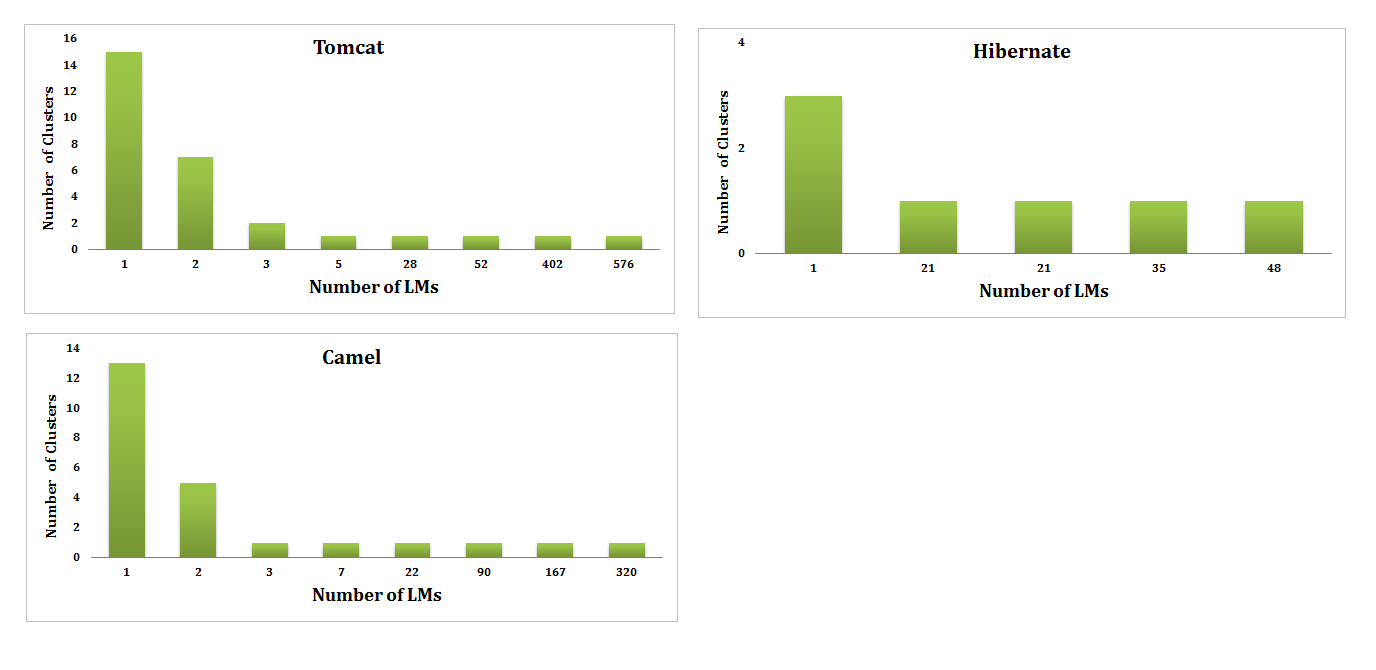
\includegraphics [width = 1\textwidth, height = 0.5\textheight] {Charts/Histograms.png}
  \caption{Histograms of the number of LMs per cluster.}
  \label{fig:histograms}
\end{sidewaysfigure}


\subsection{Analysis}  \label{analysis}
The first research question is: \emph{"Is it possible to find patterns of where log statements occur in source code?"} As shown in Table~\ref{tab_results_1}, the number of clusters has been reduced by more than 90\% in all the studied systems, indicating that developers follow some patterns for locating the log statements in source code. Furthermore, histograms depicted in Figure~\ref{fig:histograms} show that in all the studied systems, a few clusters contain a large number of LMs; however, the other clusters contain a very small number of LMs. This indicates that in these cases, developers follow a more complex or rare way of locating log statements. These exceptions might also happen due to the poor usage of logging statements in source code, which impacts the quality of the entire system negatively.

The second research question is : \emph{``What common structural characteristics do logged methods have?''}
To address this question, I manually went through the LUSs to identify the common structural characteristics of locating log statements in source code.

%a few rare exception
%ADD-> THE USAGE WITH AN EXCEPTION

\subsubsection{\emph{Categorizing logging usage}} \label{categories}
In this section, I will describe the anti-unifiers of logging usage by examining the LUSs produced by \tool{ELUS}. In general, there are five main categories of anti-unifiers in the logging usage. Each category represents one cluster of each software system that contains a large number of LMs, that is, the cluster anti-unifier represents a common way of locating log statements in source code. In the following sections, I will describe the common structural characteristics of each category represented by the anti-unifier. In addition, Figure~\ref{fig:categories} presents the number of LMs in each category and its percentage of the total number of LMs for each of the software systems. As shown in this figure, the distribution of logging categories vary from application to application, which implies that logging guidelines should be provided at application-specific level in order to establish effective logging practices.
% that their anti-unifiers are corresponded, as they have common structural characteristics. Also, these clusters
\begin{sidewaysfigure} [p]
   \centering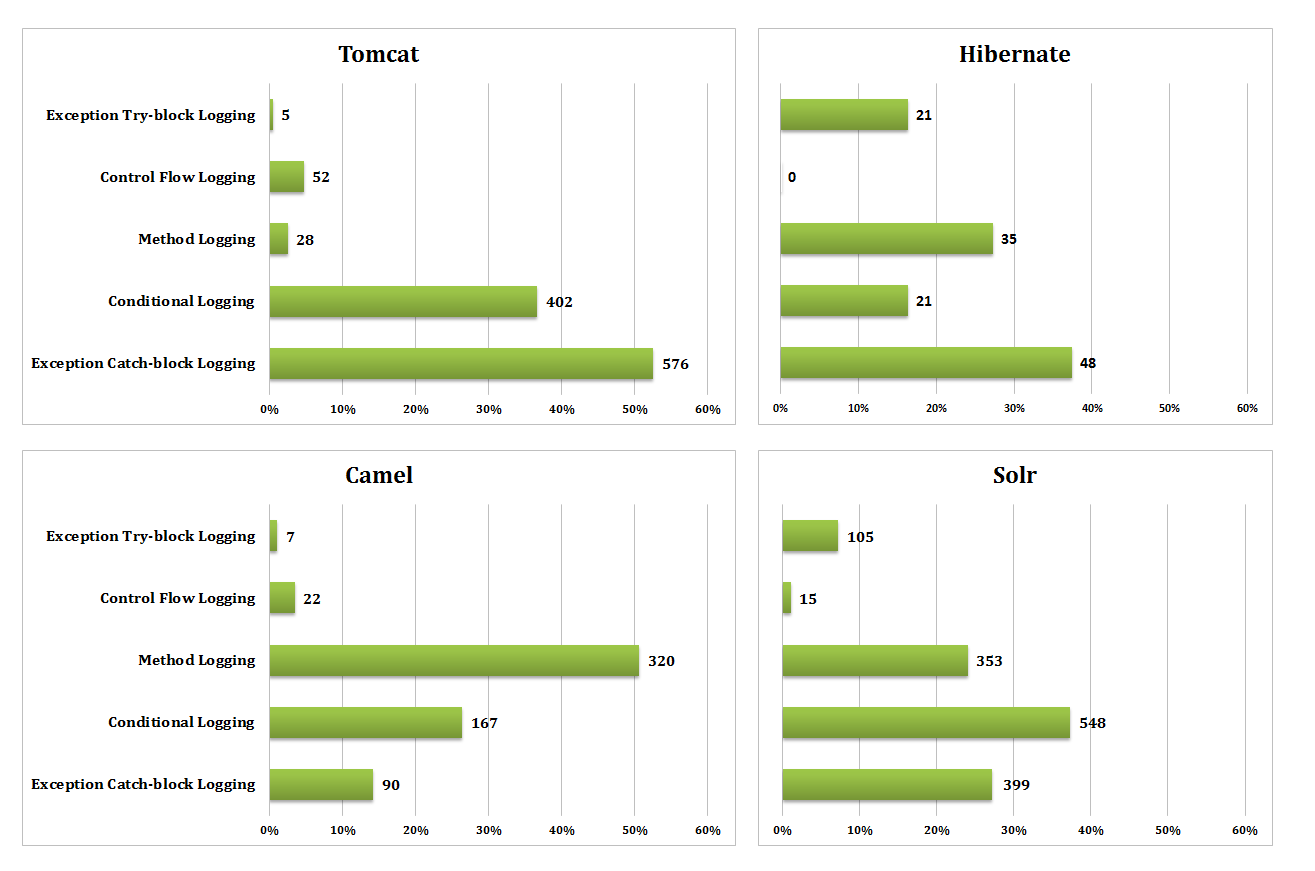
\includegraphics [width = 1\textwidth, height = 0.7\textheight]{Charts/Categories.png}
  \caption{The distribution of the categories of anti-unifiers in the logging usage.}
  \label{fig:categories}
\end{sidewaysfigure}


% how to compare?

\subsubsection{\emph{A. Exception Catch-block Logging}}  \label{Exception catch-block logging}
The main common structural characteristics of the anti-unifiers of this category are the \code{try} statements, where the log statements are located inside the body of a \code{catch} clause. As shown in Figure~\ref{fig:categories}, 14\% to 52\% of the total LMs are described by the anti-unifiers of this category, and it is the most commonly used logging usage category in the \name{Tomcat} and \name{Hibernate} software systems. The popularity of this category among all the studied systems is due to the fact that exception handling using the \code{try}/\code{catch} blocks is a common technique in the Java programming language.

%a large portion of LMs are described by the anti-unifiers of this category.

\subsubsection{\emph{B. Conditional Logging}}  \label{conditional logging}
In this category, log statements are enclosed by \code{if}-statements with their test expressions mostly among \textit{infixExpression}, \textit{methodInvocation}, or \textit{binaryExpression} nodes. The \textit{infixExpression}s mostly either check the equality of an expression to the null literal or tests the validity of the value of a variable; the \code{if}-statements testing \textit{methodInvocation}s mostly check if the return value of an invoked method is an indicator of a potential problem within a system; and the \code{if}-statements testing \textit{binaryExpression}s mostly check if a Boolean literal is incorrect. As shown in Figure~\ref{fig:categories}, 16\% to 37\% of the total LMs are described by the anti-unifiers of this category, and it is the most commonly used logging category in the \name{Solr} system.

\subsubsection{\emph{C. Outer Method Logging}}  \label{method logging}
In this category, the log statements are located inside the body of \textit{methodDeclaration} nodes but outside of other structures nested therein. A common structural characteristic of the anti-unifiers in this category is that they mostly use the \code{throw} statement to throw an exception if an error occurs. The percentage of LMs that are described by the anti-unifiers of this category ranges from 3\% to 51\%, and it is the most common logging usage category in the \name{Camel} software system. This suggests that developers use logging to record important method granularity information about the state of a software system. This information might be used later to detect the root causes of an application problem.
% %?
% throw exception



\subsubsection{\emph{D. Control Flow Logging}}  \label{Control flow logging}
In this category, the log statements are located inside the body of either \code{switch}- or \code{if}-\code{else} statements. These log statements can be used to reveal necessary information to track the location of root causes of a potential problem in a software system. According to the Figure~\ref{fig:categories}, 0\% to 5\% of the total LMs are described by the anti-unifiers of this category.


\subsubsection{\emph{E. Exception Try-Block Logging}}  \label{Exception try-block logging}
In this category, the log statements are located inside the body of the \code{try} clause of \code{try}/\code{catch} statements. These log statements can be used to record important information about the code that may throw an exception. As shown in Figure~\ref{fig:categories}, 0\% to 7\% of the total LMs of the studied systems are described by the anti-unifiers of this category.

%COMPARE SYSTEMS???
%CATEGORIES FIGURE CHANGE???

\section{Evaluation}  \label{evaluation}
%\RW{For constrained variables, the precision should be 100\%.  The fact that it is not means that there are some bugs.  There is no point in pretending otherwise; you are better off pointing this out.  It's OK: all software contains bugs.  Later, in the Discussion, you should point out that intermediate forms of constraint are possible: instead of constraining to only the exactly desired substitutions, you can constrain to the legal types of nodes (like methodInvocation) that can be used to substitute a variable.  The (still open) question is if that would yield better results than unconstrained variables.}
%\NZ{I added it to the discussion chapter}

An empirical study is conducted to evaluate the quality of the anti-unifiers generated by \name{ELUS} in describing the location of log statements in source code. Section~\ref{precision} describes the process of evaluating the precision and recall of \tool{ELUS}.


\subsection{{Calculating the precision and recall}}  \label{precision}
To find the locations in source code that are described by an anti-unifier using \tool{ELUS}, I applied the \func{Determine-Locations} algorithm, which takes the anti-unifier and a list of all methods in source code and outputs a list of methods that their AUAST matches the anti-unifier AUAST. This algorithm anti-unifies each method in the list with the anti-unifier using the \func{Antiunify} algorithm described in Section~\ref{meth-antiUnifier} (lines~2--3). If the result equals the anti-unifier, that method will be added to the list of locations matching the anti-unifier (lines~4--5). \func{Equals} is a procedure that takes two AUAST nodes and checks whether they are equal or not. To evaluate the generalizability of the anti-unifiers, I have implemented this procedure in two ways: (1) when variables are considered to be \emph{constrained}, it tests that the non-variable nodes are identical in the two AUASTs and checks if the constraints of variable are identical or not; (2) when variables are considered to be \emph{unconstrained}, it tests that the non-variable nodes are identical in the two AUASTs, but permits unconstrained variables to differ. I ran my tool on the source code of the four studied systems and applied this algorithm to find the locations in the code that matches the structure of the generated anti-unifiers. Then, the precision and recall metrics are calculated using Equations~\ref{precision_eq} and~\ref{recall_eq}, respectively.


\begin{algorithm}
\caption{\func{Determine-Locations}($\id{antiUnifier}$,$\id{methods}$) finds the locations in source code that matches an anti-unifier.}
\label{alg-determine-locations}
\begin{algorithmic}[1]
\DetermineLocations
    \State $\id{locations} \gets \{\}$
    \For {$\id{method} \in \id{methods}$}
    \State $\id{result} \gets  \func{AntiUnify}(\id{antiUnfier}, \id{method})$
		\If {$\func{Equals}(\id{result}, \id{antiUnifier})$ }	
				 	\State{$\func{Append}(\id{method}, \id{locations})$ }
		\EndIf 		
		\EndFor
 \Return $\id{locations} $  	
  \end{algorithmic}
\end{algorithm}

\begin{equation}\label{precision_eq}
\id{precision} = \frac{\id{TP}}{{\id{TP}+\id{FP}}}
\end{equation}


\begin{equation}\label{recall_eq}
\id{recall} = \frac{\id{TP}}{{\id{TP}+\id{FN}}}
\end{equation}


Where $\id{TP}$ is the number of correct locations obtained, $\id{FP}$ is the number of incorrect locations retrieved, and $\id{FN}$ is the number of correct locations that were not retrieved. Figures~\ref{fig:precision} and \ref{fig:recall} show the precision and recall results for each software system where the experiment was run once with constrained variables and once with unconstrained variables.


\begin{figure} [H]
  \centering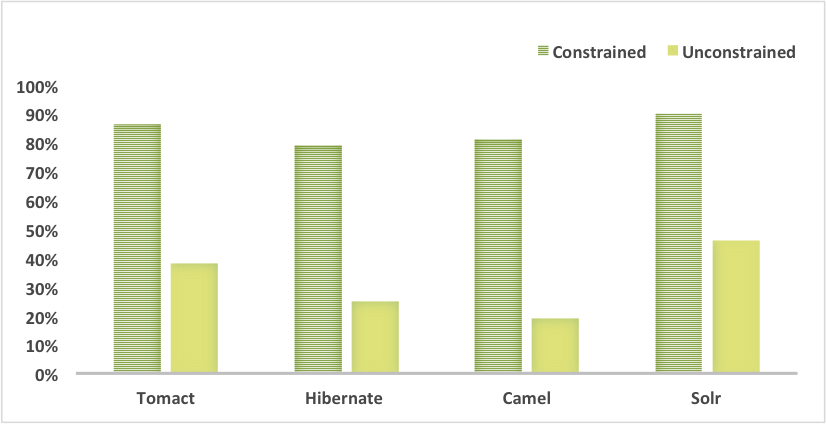
\includegraphics [width = 0.7\textwidth, height = 0.3\textheight]{Charts/Precision.png}
  \caption{The precision of \tool{ELUS}.}
  \label{fig:precision}
\end{figure}

\begin{figure} [H]
  \centering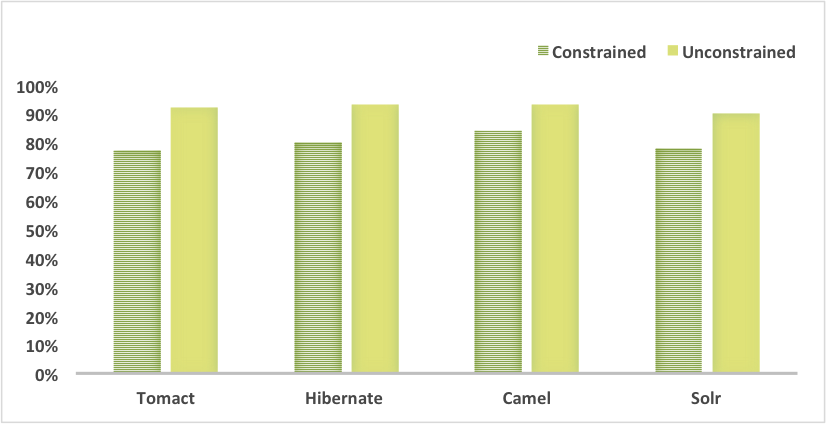
\includegraphics [width = 0.7\textwidth, height = 0.3\textheight]{Charts/Recall.png}
  \caption{The recall of \tool{ELUS}.}
  \label{fig:recall}
\end{figure}

\subsection{{Precision results}}  \label{precision-results}
The green and yellow bars in Figure~\ref{fig:precision} show the precision results when the experiment was run with constrained and unconstrained variables, respectively. I have also calculated the overall average precision of \tool{ELUS}, by averaging the precision values between the four software systems. The average precision for \tool{ELUS} is 84\% and 32\% for constrained and unconstrained variable experiments, respectively. In general, the precision for constrained variables is fairly high. The main reason behind the high precision of constrained variables is that in these cases, the variables can only be substituted with some particular nodes, which makes the anti-unifier very specific. However, there are two main reasons for the fact that precision of constrained experiment is not 100\%:
\begin{enumerate} [leftmargin=.5in]

\item \emph{Split cases}: To handle the cases containing multiple log statements, I split them into more than one case, where each contains only one logging statement (see Section~\ref{meth-multipleLogs}). However, to find the locations in source code that are described by anti-unifiers using the \func{Determine-Locations} algorithm, I compared them with all the methods in source code without splitting them into multiple cases, which results in retrieving a number of incorrect locations.

\item \emph{Software bugs}: The fact that precision results are not ideal indicates that \tool{ELUS} has some bugs. In the further work, I aim to improve these results by fixing the software bugs.
\end{enumerate}

According to the Figure~\ref{fig:precision}, the precision is fairly low for unconstrained variables. The main reason of the low precision for these cases is the fact that the unconstrained variables can be substituted by any nodes, which makes the anti-unifiers too general. As a result, the tool finds many incorrect locations the matches the anti-unifiers.





%\RW{Rewrite this according to the discussion we had in the meeting}

\subsection{{Recall results}}  \label{recall-results}
The green and yellow bars in Figure~\ref{fig:recall}  show the recall results when the experiment was run with constrained and unconstrained variables, respectively. I have also calculated the overall average recall of \tool{ELUS}, by averaging the recall values between the studied systems. The average recall for \tool{ELUS} is 80\% and 97\% for the constrained and unconstrained variable experiments, respectively. In general, when variables are constrained, \tool{ELUS} can detect many correct locations, as the recalls for all the studied systems are fairly high. Also, \tool{ELUS} can detect most of the correct locations in source code when no constraints are taken on variable nodes.

The main reason behind \tool{ELUS}'s failure to detect the correct locations is the potential complexities in constructing anti-unifiers from a large set of source code fragments. As in some cases, the anti-unifier might not maintain the correct locations of nodes in the AST hierarchy, and thus \tool{ELUS} would not be able to successfully construct the anti-unifiers of logging usage in source code.
%detect correct locations of log statements in the source code.
%?
%\RW{Ah, I see that you have a note in here about the intermediate constraints.}

%ADDDDD
% assess the generalizability of the anti-unifiers --> in between
%In general,  the tool retrieved some locations matching the anti-unifiers, while in fact they do not match.
%the tool failed to retrieve the correct locations, and in other cases



\section{Usage}  \label{usageELUS}
The insightful findings of my characterization study regarding the logging usage in several real-world software systems can be used to enhance the quality of existing logging practices by providing some logging guidelines for developers. For example, Figure~\ref{inapproprate-ex1} shows a logged method that belongs to a singleton cluster in my experiment. This \name{Java} method is an example of a poor usage of a log statement in code, as the list \code{liveNodes} can be \code{null}, and thus a \code{NullPointerException} can be thrown causing a system crash. To enhance the quality of the logging usage in this code snippet, a developer my look at our findings to be informed of how usually other developers locate log statements in similar situations. As noted in Section~\ref{categories}, to avoid the \code{NullPointerException}, developers usually insert the logging call into the body of an \code{if} statement to check if the value of the variable needed to be logged is not \code{null}. Hence, she can improve the quality of the logging usage in this example by inserting the logging call inside an \code{if} statement and log the needful information if the value of the list \code{liveNodes} is not \code{null} (lines~6--8 of Figure~\ref{approprate-ex1}). This example demonstrates how these findings can be used in practice to improve the quality of logging practices.
% in real-world application.


\begin{figure}[p]
\def\baselinestretch{1}
\begin{lstlisting}[escapechar=!]
public void setUp() throws Exception {
    SolrZkClient zkClient=new SolrZkClient(zkServer.getZkAddress(),AbstractZkTestCase.TIMEOUT);
    for (int i=0; i < 30; i++) {
       List<String> liveNodes=zkClient.getChildren("/live_nodes",null,true);
       Thread.sleep(1000);
       !\colorbox{yellowGreen}{log.info("Waiting for more nodes to come up, now: " + liveNodes.size());}!
    }
}
\end{lstlisting}
\caption[An example of an inappropriate usage of a log statement in a Java method.]{An example of an inappropriate usage of a log statement in a Java method.\label{inapproprate-ex1}}
\end{figure}



\begin{figure}[p]
\def\baselinestretch{1}
\begin{lstlisting}[escapechar=*]
public void setUp() throws Exception {
    SolrZkClient zkClient=new SolrZkClient(zkServer.getZkAddress(),AbstractZkTestCase.TIMEOUT);
    for (int i=0; i < 30; i++) {
       List<String> liveNodes=zkClient.getChildren("/live_nodes",null,true);
       Thread.sleep(1000);
       *\colorbox{yellowGreen}{if (liveNodes != null) }*
         *\colorbox{yellowGreen}{log.info("Waiting for more nodes to come up, now: " + liveNodes.size()); }*
    }
}
\end{lstlisting}
\caption[Modified Java method of Figure~\protect\ref{inapproprate-ex1} for the purpose of enhancing the logging usage.]{Modified Java method of Figure~\ref{inapproprate-ex1} for the purpose of enhancing the logging usage.\label{approprate-ex1}}
\end{figure}
   % !\colorbox{yellowGreen}{}}!
  %!\colorbox{yellowGreen}{if (liveNodes  null) { }!

\section{Summary}
I conducted an experimental study to characterize the location of log statements by applying my tool on the source code of four full software systems that make use of the \name{Apache log4j} logging framework. My tool inputs the source code of these systems, extracts ASTs of LMs, applies the proposed anti-unification and clustering algorithms, and outputs the anti-unifier for each cluster. I also conducted an experimental study to evaluate the precision and the recall of \tool{ELUS} in constructing the anti-unifiers that describe the location of log statements in source code. This experiment shows that \tool{ELUS} has achieved promising results in terms of precision and recall. Furthermore, the results taken from the characterization experiment shows that there are common ways of locating log statements. I manually examined the detailed view of structural generalizations and categorized the anti-unifiers of logging usage. In the last section of this chapter, I provided an example to demonstrate the usage of the findings of my characterization study in practice.


% In summary, this experiment shows that \tool{ELUS} has achieved promising results in terms of precision and recall metrics.

% My analysis has resulted in ... different anti-unifiers in the logging usage.

% figure out the common structural characteristics of LMs in each cluster.
%I found out that most log statements are embedded inside ....

\addtocontents{toc}{\protect\addvspace{10pt}}
\chapter{Discussion}  \label{diss}

In this chapter, we discuss the validity of our evaluation and the characterization study (Section~\ref{threads}), the limitations and pitfalls of the approach and our tool support (Section~\ref{limitations}), and a number of remaining issues including: the other applications of our tools' underlying framework (Section~\ref{other_applications}); the usage of anti-unification theory (Section~\ref{auTheory}).

\section{Threats to validity}  \label{threads}
Prior to applying our tool for characterizing logging usage in real-world software systems, we have conducted three experiments to investigate the effectiveness of our proposed approach. However, there are several potential threats regarding the validity of these experiments. First, the results of our manual examination might be biased, as I determined the correct correspondences between ASTs and the correct way of classifying the set of ASTs in our test suite based on a similarity measurement. To limit the bias, other people can be involved to double check the accuracy of my manual inspection in a future work. Secondly, the experiments have examined one test suite containing a set of LJMs from a real-world software system, though different test suites may generate different results. Although I cannot claim that the LJMs in my test suite are a good representative of all LJMs in real-world software systems, the results are still promising, as logging calls are used in various ways in Java methods of my test suite, and have sufficed to indicate the effectiveness of my approach in constructing structural generalizations. Another potential thread is that the successful rate of detecting correspondences by our tool might happen accidentally only for our test suite. To resolve this doubt, we examined the cases where our tool fails to detect correct correspondences and we found that the failures are due to the fundamental limitations and complexities in the construction of structural generalization through the use of structural correspondence. That is, our tool creates structural generalizations successfully with regard to what our algorithm should generate.
%, and the assumptions taken in developing the algorithms.
%CITATION POPULARITY!!!
%There are several threats to the validity of our characterization study.
A potential thread to the validity of our characterization study is the degree to which our sample set of software systems is a good representation of all real-world logging usage. To address this issue, we selected various open-source software projects in terms of application, including a programming text editor, a web server, and an application server. These software systems are among the most popular applications in their own product category, and they all have at least 10 years of history in software development. However, our findings might not be able to reflect the characteristics of logging usage in other types of systems such as commercial software, or software written in other programming languages. 
%citation???
%application of softwares???

\section{Our tool output}  \label{limitations}
In addition, there are some issues that the approximation approach and our tool support is not able to handle perfectly, including node ordering mismatch, and the management of conflicts happened in constructing the anti-unifiers.

\subsection{Node ordering mismatch}  \label{mismatch} 
Our anti-unification algorithm does not guarantee to maintain the correct sequence of statements in the body of methods when anti-unifying two method declaration nodes, since the order of statement nodes is not considered in determining the best correspondences. For example, consider we have two corresponding methods $\id{method_1}$ and $\id{method_2}$ embodying {$\id{a_1}$, $\id{a_2}$, $\id{a_3}$} and {$\id{b_1}$, $\id{b_2}$} sequences of statements, respectively. If our tool finds that the $\id{b_1}$ and $\id{b_2}$ nodes are the best correspondences for the $\id{a_3}$ and $\id{a_1}$ nodes respectively, the output generalization view for the set of statement nodes would be {$\id{a_1}$-or-$\id{b_2}$, $\id{a_2}$-or-$\NIL{}$, $\id{a_3}$-or-$\id{b_1}$}. Therefore, the generalization view does not preserve the correct ordering of nodes in the original structures.


\subsection{handle conflicts in constructing the anti-unifiers}  \label{conflicts} 
The decisions we have made to resolve the conflicts occurred in constructing structural generalizations might affect the accuracy of our results.
For example, in situations where we have two correspondences with the same similarity value in the ordered list of correspondence connections, our approach picks the one which involves two subtrees with higher number of leaves, though it might be not the best choice for all cases. 
In addition, we consider AST hierarchies to perform anti-unification. That is, our algorithm does not anti-unify two nodes if their parent nodes are not found to be corresponded. As a result, situations can occur where in fact two nodes should be anti-unified with each other, while they are not anti-unified by the tool. Though these decisions leads us to get approximate results, they helped to limit the complexity of our approach allowing the implementation of it as a practical solution.

 % add semantic to structural information to detect correspondences?? 
%limited typing information to determine correspondences by %Jigsaw
%\item Our tool does not guarantee the correctness of determining the best correspondences due to
%\begin{itemize} [leftmargin=.3in]
%\item the various conflicts that happen
%\item limited typing information to determine correspondences by %Jigsaw
%\end{itemize}
%\item Structural generalizations constructed by our tool are not in %the form of executable code
%[leftmargin=.3in]\end{itemize}


\section{Other applications}  \label{other_applications}
Any applications that are involved in the inference of structural patterns in source code even infrequently-used patterns might benefit from our tool’s underlying framework.
%% EXAMPLE??? 
Furthermore, understanding the commonalities and differences between source code fragments has application in several areas of software engineering, such as code clone detection, API usage pattern collation, recommending replacements for API migration, and merging different branches of version control systems. Our tool`s functionality to construct a detailed view of structural generalizations to represent the similarities and differences between a set of source code fragments via structural correspondence could be used to improve the results of these studies as well.
%edit!!!
\section{Applications of anti-Unification}  \label{auTheory}
Our study demonstrates the application of an extended from of anti-unification (HOAUMT) to infer usage patters of log statements in source code via the creation of structural generalizations. Anti-unification and its extensions have been already applied to solve several theoretical and practical problems, such as analogy making [Schmidt, 2010], determining lemma generation in equational inductive proofs [Burghardt, 2005], and detecting the construction laws for a sequence of structures [Burghardt, 2005]. 
%CITATION??

Higher-order anti-unification modulo theories can be used to create generalizations in different contexts, and therefore the set of equational theories should be developed particularly for the higher-order structure used in each problem context. That is, the utility of these theories are highly dependent on how well they allow the incorporation of semantic knowledge of structures. In addition, these theories should ensure that only a finite number of anti-instances exist for each structure. Taking all these considerations into account enables HOAUMT to anti-unify sets of structures, which is useful for a particular context. The practical tests I have conducted through the application of my tool on a test suite demonstrate that our approximation of HOAUMT was successful in constructing structural generalizations required to solve our problem.
%

%?????????
The problem of my study is different, but this work shows how the Jigsaw framework could be useful in constructing structural generalizations to solve a particular problem context via the determination of structural correspondences between two ASTs. The application of HOAUMT to construct structural generalizations via structural correspondences is novel to the problem of extracting usage patterns of log statements in source code.
Finally, we made a comparison between our tool and the Jigsaw tool, which were developed for various applications, but part of the implementation of Jigsaw was successfully applied to solve our problem context.



\section{Summary}  \label{diss-summary}
We discussed the potential threads to validity of our evaluation and characterization study. To limit the bias of the experiments we conducted to evaluate the effectiveness of our approach and the tool support, we selected our test cases form a real system with various levels of similarity in the usage of logging calls. Furthermore, we examined the failed test cases to assure that our tool works when it should work with regard to the proposed algorithm. We will also make our test suite available for public examination to check the accuracy of our manual inspection. For our characterization study, we selected various software systems in terms of functionality that are widely used by many developers for a long period of time. We also discussed the remaining issues with our tool support including node ordering, …, and … that can be resolved in future as the extensions of our work.

This work aim to provide a detailed view of structural generalizations constructed from a set of source code fragments that use log statements via structural correspondence and clustering. However, we discussed that any other applications involved in the inference of structural usage patterns of a particular statement or the detection of commonalities and differences between a set of source code fragments could benefit from our tool’s underlying framework.

We also argued how higher-order anti-unification modulo theories can be effectively approximated for various applications by means of developing an appropriate set of equational theories particularly for the higher-order structure used in each problem context. 

\addtocontents{toc}{\protect\addvspace{10pt}}
\chapter{Related Work}  \label{rw}
In this chapter, we review related work to the topics of our study including: the application of logging in real-world software systems (Section~\ref{logging}), determining correspondences in source code (Section~\ref{ch7-corr}), data mining approaches to extract API usage patterns (Section~\ref{ch7-usage-patterns}), anti-unification and its application to detect strcutural correspondences and construct generalizations (Section~\ref{ch7-au}), and clustering (Section~\ref{ch7-clustering}).
% constructing the structural generalizations (Section~\ref{ch7-generalization}
\section{Usage of logging}  \label{logging}
Logging is a conventional programming practice to record a software system's runtime information that can be used in post-modern analysis to trace the root causes of systems' activities. Log analysis is most often performed for failure diagnosis, system behavioral understanding, system security monitoring, and performance diagnostics purposes as described below:
\begin{itemize} [leftmargin=0.5in]
\item \textbf{Log analysis for failure diagnosis: }\citet{xu2009detecting} use statistical techniques to learn a decision tree based signature from console logs and then utilize the signature to diagnose anomalies. SherLog \cite{yuan2010sherlog} uses failure log messages to infer the source code paths that might have been executed during a failure.
\item \textbf{Log analysis for system behavior understanding: }\citet{fu2013contextual} present an approach for understanding system behavior through contextual analysis of logs. They first extracted execution patterns reflected by a sequence of system logs and then utilized the patterns to find contextual factors from logs that causes a specific system behavior. The Linux Trace Toolkit \cite{yaghmour2000measuringandcharacter} was created to record and analyze system behavior by providing an efficient kernel-level event logging infrastructure. A more flexible approach is taken by DTrace \cite{cantrill2004dynamic} which allows dynamic modification of kernel code.
\item \textbf{Log analysis for system security monitoring: }\citet{bishop1989model} proposes a formal model of system's security monitoring using logging and auditing. \citet{peisert2007toward} have developed a model that demonstrates a mechanism for extracting logging information to detect how an intrusion occurs in software systems.
%have developed?
% Jiang et al. [2009b] present an approach to automatically detect problems of load tests by mining the execution logs of an application. Many software systems must be load tested for their functional and performance problems diagnosis.
\item \textbf{Log analysis for performance diagnosis: }\citet{nagaraj2012structured} developed an automated tool to assist developers in diagnosis and correction of performance issues in distributed systems by analyzing system behaviors extracted from the log data.
\end{itemize}

\citet{jiang2009understanding} study the effectiveness of logging in problem diagnosis. Their study shows that customer problems in software systems with logging resolve faster than those without logging by investigating the correlations between failure root causes and diagnosis time. Despite the importance of logging for software development and maintenance, few studies have been conducted in pursuit of understanding logging usage in real-world software. \citet{yuan2012characterizing} provides a quantitative characteristic study to investigate log message modifications on four open-source software systems by mining their revision history. Their study shows that developers spend great effort modifying log statements as after-thoughts, which indicates that they are not satisfied with the log quality in their first attempt. They also characterize where developers spend most of their time in modifying the log messages.

\citet{yuan2012conservative} study the problem of lack of log messages for error diagnosis and suggests to log when generic error conditions happens. LogEnhancer \cite{yuan2012improving} automatically enhances existing log messages by detecting variables containing important values and inserting them into the log messages. However, these studies only consider source code fragments containing bugs that are needed to be logged and do not consider the other code fragments with no bugs but still needed to be logged. Moreover, these studies mainly research log message modifications and potential enhancements of them, however, the focus of this study is on understanding where logging calls are used in source code.
% where to log
% Sadi

\section{Correspondence}  \label{ch7-corr}
Several studies have been conducted to find the similarities and differences between source code fragments. \citet{baxter1998clone} develop an algorithm to detect code clones in source code that uses hash functions to partition subtrees of ASTs of a program and then find common subtrees in the same partition through a tree comparison algorithm. \citet{apiwattanapong2004differencing} present a top-down approach to detect differences and correspondences between two versions of a Java program, through comparison of the control flow graphs created from source code. \citet{holmes2005strathcona} recommend relevant code snippet examples from a source code repository for the sake of helping developers to find examples of how to use an API by heuristically matching the structure of the code under development with the code in the repository. Coogle \cite{sager2006detecting} is developed to detect similar Java classes by converting ASTs to a normalized format and then comparing them through tree similarity algorithms. However, none of these approaches construct a detailed view of structural generalizations needed in our context.
%explain more why not ??
%Umami
 
\citet{2014:uofc:cossette} present a new approach, called Matching via Structural generalization (MSG), to recommend replacements for API migration. They used Jigsaw to find structural correspondences, however, the proposed algorithm does not suffice to construct structural generalizations that represent the detailed commonalities and differences of a set of source code fragments with special attention to log statements, which is required to solve our problem.
%. It also does not take the required constraints in determining correspondences needed to solve our problem.

\section{API usages patterns}  \label{ch7-usage-patterns}
Various data mining approaches have been used to extract API usages patterns out of source code such as unordered pattern mining and sequential pattern mining \cite{robillard2013automated}. Unordered pattern mining, such as association rule mining and itemset mining, extracts a set of API usage rules without considering their order \cite{agrawal1994fast}. CodeWeb \cite{michail2000data} uses data mining association rules to identify reuse patterns between a source code under development and a specific library. PR-Miner \cite{li2005pr} uses frequent itemset mining to extract implicit programming rules from source code and detect violations. The sequential pattern mining technique is different from the unordered one in the way that it considers the order of API usage. As an example, MAPO \cite{xie2006mapo} combines frequent subsequence mining with clustering to extract API usage patterns from source code. 

Another technique for extracting API usage patterns is through statistical source code analysis. For example, PopCon \cite{holmes2008newbie} is a tool developed to help developers understanding how to use APIs in their source code through calculating popularity statistics for each API of a library. \citet{acharya2007mining} present a framework to extract API usage scenarios as partial orders, as specifications were extracted from frequent partial orders. They adapted a compile time model checker to generate control-flow-sensitive static traces of APIs, from which API usage scenarios were extracted. However, none of these approaches suffice to construct detailed structural generalizations needed in our context.
%However, none of these approaches suffice to determine the detailed structural correspondences.
\section{Anti-unification}  \label{ch7-au}
Anti-unification is the problem of finding the most specific generalization of two terms. First-order syntactical anti-unification was introduced by \citet{plotkin1970note} and \citet{reynolds1970transformational}, independently. \citet{burghardt1996implementing} extend the notion of anti-unification to E-anti-unification to incorporate background knowledge to syntactical anti-unification, which is required for some applications. Anti-unification and its extensions have been applied in various studies for program analysis. \citet{bulychev2009evaluation} suggest an anti-unification algorithm to detect clones in ASTs. Their approach consists of three stages: first, identifying similar statements through anti-unification and grouping them into clusters; second, determining similar sequences of statements with the same cluster identifier; third, refining candidate statement sequences using an anti-unification based similarity measurement to generate final clones. However, their approach does not construct structural generalizations.
%?

\citet{2007:esec_fse:cottrell} propose Breakaway to automatically determine structural correspondences between a pair of ASTs to create a generalized correspondence view. However, their approach does not allow the determination of the best structural correspondence for each AST node required to our context. \citet{2008:fse:cottrell} develop Jigsaw to help developers integrate small-scale reused code into their own source code by determining structural correspondences through the application of higher-order anti-unification modulo theories. Though I used the Jigsaw framework to find potential correspondences between AST nodes, their approach does not suffice to construct structural generalizations of a set of source code fragments by considering the limitations of this study in determining correspondences.

%\item Sadi [2011] proposed an anti-unification algorithm to characterize the location of logging usages in the source code, however,
%\begin{itemize} [leftmargin=.3in]
%\item he has not applied anti-unification appropriately!!! \RW{You would need to explain what that means}
% Higher-order anti-unification modulo theories is formally undecidable [Burghardt, 2005].

\section{Clustering}  \label{ch7-clustering}

%optimal clusters
Clustering is an unsupervised machine mining technique that aims to organize a collection of data into clusters, such that intra-cluster similarity is maximized and the inter-cluster similarity is minimized \cite{karypis1999chameleon,grira2004unsupervised}. We divided existing clustering approaches into two major categories: partitional clustering and hierarchical clustering. Partitional clustering try to classify a data set into $k$ clusters such that the partition optimizes a pre-determined criterion \cite{karypis1999chameleon}. The most popular partitional clustering algorithm is k-means, which repeatedly assigns each data point to a cluster with the nearest centroid and computes the new cluster centroids accordingly until a pre-determined number of clusters is obtained \cite{bouguettaya2015efficient}. However, k-means clustering algorithm is not a good fit to our problem, as it requires to predefine the number of clusters we need to come up with, which is not reasonable in our context. %?

Hierarchical clustering algorithms produce a nested grouping of clusters, with single point clusters at the bottom and an all-inclusive cluster at the top \cite{karypis1999chameleon}. Agglomerative hierarchical clustering is one of the main stream clustering methods \cite{day1984efficient} and has applications in document retrieval \cite{voorhees1986implementing} and information retrieval from a search engine query log \cite{beeferman2000agglomerative}. It starts with singleton clusters, where each contains one data point. Then it repeatedly merges the two most similar clusters to form a bigger one until a pre-determined number of clusters is obtained or the similarity between the closest clusters becomes below a pre-determined threshold value. Hierarchical clustering algorithms work implicitly or explicitly with the $n \times n$ similarity matrix such that an element in row $i$ and column $j$ represents the similarity between the $i^{\text{th}}$ and the $j^{\text{th}}$ clusters \cite{karypis1999chameleon}.
% agglomerative hierarchical or hierarchical ???

There are various versions of agglomerative hierarchical algorithms that mainly differ in how they update the similarity between clusters. There are various methods to measure the similarity between clusters, such as single linkage, complete linkage, average linkage, and centroids [Rasmussen, 1992]. In the single linkage method, the similarity is measured by the similarity of the closest pair of data points of two clusters. In the complete linkage method, the similarity is computed by the similarity of the farthest pair of data points of two clusters. In the average linkage method, the similarity is measured by the average of all pairwise similarities between data points of two clusters. In the centroids methods, each cluster is represented by a centroid of all data points in the cluster, and the similarity between two clusters is measured by the similarity of the clusters' centroids.
However, in our application, each cluster is composed of one AUAST, and the similarity between two clusters is measured by the similarity between the clusters' AUASTs, which is the ratio of the number of common pieces over the total number of pieces of their anti-unifier.
% (see Section~\ref{meth-similarity}). 
%optimal clusters- read dr. denzinger email
%similarity and distance two sides of a coin
% k-means,the predetermined criterion is met
% Hierarchical clustering approaches produce clusters of higher quality, however, these approaches suffer from high time cost[Bouguettay]

\section{Summary}  \label{back-summary}
%machine learning, other generalization approaches

Despite the great importance of logging and its various applications in software development and maintenance, few studies have focused on understanding logging usage in source code.
Some work has been done on characterizing log messages modifications made by developers and to help them enhance the content of log messages. However, to my knowledge, no study has been conducted on characterizing where logging is used in source code via structural generalization and clustering. Several data mining and statistical source code analysis techniques have been used to extract API usage patterns, however, none of them enable us to construct the detailed structural generalizations of a set of source code fragments. On the other hand, using higher-order anti-unification modulo theories and an agglomerative hierarchical clustering algorithm allow us to construct generalizations representing the commonalities and differences between ASTs of logged Java methods and grouping them into clusters based on structural correspondence.


\addtocontents{toc}{\protect\addvspace{10pt}}
\chapter{Conclusion}  \label{conc}
\begin{itemize} [leftmargin=.01in]
\item Determining the detailed structural similarities and differences between source code fragments is a complex task
\item It can be applied to solve several source code analysis problems, for example, characterizing logging practices
\item logging is a pervasive practice and has various applications in software development and maintenance
\item However, it is a challenging task for developers to understand how to use logging calls in the source code
\item We have presented an approach to characterize where logging calls happen in the source code by means of structural generalization
\item We have developed a prototype tool that:
\begin{itemize} [leftmargin=.3in]
\item detects potential structural correspondences using anti-unification
\item uses several constraint to remove the correspondences that are not suited to our application
\item determines the best correspondences with the highest similarity
\item constructs the structural generalizations using anti-unification
\item classifies the entities using a measure of similarity
\end{itemize}
\item An experiment is conducted to evaluate our approach and tool
\item Our experiment found that ...
\item An experiment is conducted to characterize logging usage in three software systems
\item In summary, our study makes the following contributions:
\begin{itemize} [leftmargin=.3in]
\item …
\item …
\end{itemize}

\section{Future Work}  \label{fw}
\item Future extensions could be applied to resolve the pitfalls of this study:
\begin{itemize} [leftmargin=.3in]
\item Data flow analysis techniques: to resolve the problem of inaccurate statement ordering
\item Further analysis: to detect and resolve all the conflicts happen in deciding the best correspondences
\end{itemize}
\item To further validate our findings from the source code analysis:
\begin{itemize} [leftmargin=.3in]
\item a survey can be conducted to ask developers on the factors they consider when they want to decide on where to log
\end{itemize}
\item Characterizing logging usage could be a huge step towards
\begin{itemize} [leftmargin=.3in]
\item improving logging practices by providing some guidelines that might help developers in making decisions about where to
log.
\item developing recommendation support tools:
\begin{itemize} [leftmargin=.3in]
\item to save developers\textquotesingle time and effort
\item to improve the quality of logging practices
\end{itemize}
\end{itemize}
\end{itemize} 

\bibliographystyle{plainnat}
\global\def\newblock{\hskip .11em plus .33em minus -.07em} %Avoids a latex complaint

% When you are working on the document, comment out Rob's line and uncomment out Narges's line, but don't delete either...

% NZ:
%\bibliography{../../../../bibtex/full,../../../../bibtex/references,../../../../bibtex/lsmr,mybiblio}
% RW:
%\bibliography{../../../../workspace/bibtex/full,../../../../workspace/bibtex/references,../../../../workspace/bibtex/lsmr,mybiblio}
\bibliography{../../../../workspace/bibtex/full,../../../../workspace/bibtex/references,../../../../workspace/bibtex/lsmr,mybiblio}



%\appendix
%%\fancyhead[RO,LE]{\thepage}
%\fancyfoot{}

\chapter{Logged Methods in Each Cluster of the Clustering Evaluation}\label{append}

\begin{table}[!tbh]
\centering\caption{LMs in the cluster $C_1$}
\begin{tabular}{ll}\toprule
Class&Method\\\midrule
\lstinline/SomeClass/&\raisebox{-2pt}{\lstinline/foo(int)/}\\
\lstinline/SomeClass/&\raisebox{-2pt}{\lstinline/foo(int)/}\\
\lstinline/SomeClass/&\raisebox{-2pt}{\lstinline/foo(int)/}\\
\lstinline/SomeClass/&\raisebox{-2pt}{\lstinline/foo(int)/}\\
\bottomrule
\end{tabular}
\end{table}

\begin{table}[!tbh]
\caption{LMs in the cluster $C_2$}
\centering\begin{tabular}{ll}\toprule
Class&Method\\\midrule
\lstinline/SomeClass/&\raisebox{-2pt}{\lstinline/foo(int)/}\\
\lstinline/SomeClass/&\raisebox{-2pt}{\lstinline/foo(int)/}\\
\lstinline/SomeClass/&\raisebox{-2pt}{\lstinline/foo(int)/}\\
\lstinline/SomeClass/&\raisebox{-2pt}{\lstinline/foo(int)/}\\
\bottomrule
\end{tabular}
\end{table}

\begin{table}[!tbh]
\caption{LMs in the cluster $C_3$}
\centering\begin{tabular}{ll}\toprule
Class&Method\\\midrule
\lstinline/SomeClass/&\raisebox{-2pt}{\lstinline/foo(int)/}\\
\lstinline/SomeClass/&\raisebox{-2pt}{\lstinline/foo(int)/}\\
\lstinline/SomeClass/&\raisebox{-2pt}{\lstinline/foo(int)/}\\
\lstinline/SomeClass/&\raisebox{-2pt}{\lstinline/foo(int)/}\\
\bottomrule
\end{tabular}
\end{table}

\end{document}

